% Options for packages loaded elsewhere
\PassOptionsToPackage{unicode}{hyperref}
\PassOptionsToPackage{hyphens}{url}
\PassOptionsToPackage{dvipsnames,svgnames,x11names}{xcolor}
\documentclass[
  vietnamese,
  12pt,
  a4paper,
]{article}
\usepackage{xcolor}
\usepackage[left=2.5cm,right=2cm,top=2.2cm,bottom=2.2cm]{geometry}
\usepackage{amsmath,amssymb}
\setcounter{secnumdepth}{-\maxdimen} % remove section numbering
\usepackage{iftex}
\ifPDFTeX
  \usepackage[T1]{fontenc}
  \usepackage[utf8]{inputenc}
  \usepackage{textcomp} % provide euro and other symbols
\else % if luatex or xetex
  \usepackage{unicode-math} % this also loads fontspec
  \defaultfontfeatures{Scale=MatchLowercase}
  \defaultfontfeatures[\rmfamily]{Ligatures=TeX,Scale=1}
\fi
\usepackage{lmodern}
\ifPDFTeX\else
  % xetex/luatex font selection
  \setmainfont[]{Times New Roman}
  \setsansfont[]{Arial}
  \setmonofont[]{Consolas}
\fi
% Use upquote if available, for straight quotes in verbatim environments
\IfFileExists{upquote.sty}{\usepackage{upquote}}{}
\IfFileExists{microtype.sty}{% use microtype if available
  \usepackage[]{microtype}
  \UseMicrotypeSet[protrusion]{basicmath} % disable protrusion for tt fonts
}{}
\makeatletter
\@ifundefined{KOMAClassName}{% if non-KOMA class
  \IfFileExists{parskip.sty}{%
    \usepackage{parskip}
  }{% else
    \setlength{\parindent}{0pt}
    \setlength{\parskip}{6pt plus 2pt minus 1pt}}
}{% if KOMA class
  \KOMAoptions{parskip=half}}
\makeatother
\usepackage{longtable,booktabs,array}
\usepackage{caption}
\captionsetup[table]{skip=6pt}
\newcounter{none} % for unnumbered tables
\usepackage{calc} % for calculating minipage widths
% Correct order of tables after \paragraph or \subparagraph
\usepackage{etoolbox}
\makeatletter
\patchcmd\longtable{\par}{\if@noskipsec\mbox{}\fi\par}{}{}
\makeatother
\ifLuaTeX
\usepackage[bidi=basic,shorthands=off]{babel}
\else
\usepackage[bidi=default,shorthands=off]{babel}
\fi
\ifPDFTeX
\else
\babelfont{rm}[]{Times New Roman}
\fi
\ifLuaTeX
  \usepackage{selnolig} % disable illegal ligatures
\fi
\setlength{\emergencystretch}{3em} % prevent overfull lines
\providecommand{\tightlist}{%
  \setlength{\itemsep}{0pt}\setlength{\parskip}{0pt}}
\usepackage{xurl}
\usepackage{fvextra}
\usepackage{tikz}
\usepackage{pdflscape}
\usepackage{fancyhdr}
\usepackage{needspace}
\usepackage{etoolbox}
\usepackage{titlesec}
\usepackage{setspace}
\usepackage{placeins}
\urlstyle{tt}
\setstretch{1.18}
\setlength{\parindent}{0pt}
\setlength{\parskip}{0.42em}
\setlength{\emergencystretch}{3em}
\setcounter{tocdepth}{2}
\renewcommand{\contentsname}{MỤC LỤC}
\AtBeginDocument{\hypersetup{colorlinks=true,linkcolor=black,urlcolor=blue!50!black,pdfborder={0 0 0}}}
\hyphenpenalty=10000
\pagestyle{fancy}
\fancyhf{}
\fancyhead[L]{\footnotesize VietFood68 — YOLO11s}
\fancyhead[R]{\footnotesize Báo cáo thực nghiệm}
\fancyfoot[C]{\thepage}
\renewcommand{\headrulewidth}{0.3pt}
\setlength{\headheight}{15pt}
\titleformat{\section}{\Large\bfseries}{\thesection}{0em}{}
\titleformat{\subsection}{\large\bfseries}{\thesubsection}{0em}{}
\titlespacing*{\section}{0pt}{1.4em}{0.65em}
\titlespacing*{\subsection}{0pt}{1.0em}{0.4em}
\AtBeginEnvironment{Verbatim}{\vspace{0.35em}}
\AtEndEnvironment{Verbatim}{\vspace{0.35em}}
\usepackage{bookmark}
\IfFileExists{xurl.sty}{\usepackage{xurl}}{} % add URL line breaks if available
\urlstyle{same}
% fallback for those not using the hyperref driver hyperxmp:
\makeatletter
\@ifundefined{xmpquote}{\newcommand{\xmpquote}[1]{#1}}{}
\makeatother
\hypersetup{
  pdflang={vi},
  colorlinks=true,
  linkcolor={Maroon},
  filecolor={Maroon},
  citecolor={Blue},
  urlcolor={Blue},
  pdfcreator={LaTeX via pandoc}}

\author{}
\date{}

\begin{document}

\hypersetup{pageanchor=false}
\begin{titlepage}
\centering
{\large ĐẠI HỌC QUỐC GIA HÀ NỘI\par}
{\large\bfseries TRƯỜNG ĐẠI HỌC KHOA HỌC TỰ NHIÊN\par}
\vspace{0.5cm}
{\normalsize KHOA TOÁN — CƠ — TIN HỌC\par}
\vspace{1.2cm}
\rule{0.8\linewidth}{0.7pt}\par
\vspace{0.8cm}
{\Large\bfseries BÁO CÁO DỰ ÁN\par}
\vspace{0.8cm}
{\LARGE\bfseries HUẤN LUYỆN VÀ ĐÁNH GIÁ MÔ HÌNH YOLO11s CHO PHÁT HIỆN THỰC PHẨM VIỆT NAM TRÊN DỮ LIỆU VIETFOOD68\par}
\vspace{0.8cm}
\rule{0.8\linewidth}{0.7pt}\par
\vfill
\begin{flushleft}
\begin{tabular}{@{}p{0.31\linewidth}p{0.66\linewidth}@{}}
Lĩnh vực & Trí tuệ nhân tạo – Thị giác máy tính \\[0.5em]
Sinh viên thực hiện & Nguyễn Ngọc Kiều Trinh \\[0.5em]
Lớp & K70A2 – Khoa Toán – Cơ – Tin học \\[0.5em]
Đơn vị & Trường Đại học Khoa học Tự nhiên, Đại học Quốc gia Hà Nội \\[0.5em]
Giảng viên hướng dẫn & Chưa được cung cấp \\[0.5em]
Ngày cập nhật thực nghiệm & 12/10/2026 \\[0.5em]
Mã lần huấn luyện & vietfood68\_5070-2 \\[0.5em]
\end{tabular}
\end{flushleft}
\vfill
{\normalsize Hà Nội, tháng 10 năm 2026\par}
\end{titlepage}
\pagenumbering{arabic}
\hypersetup{pageanchor=true,pdftitle={HUẤN LUYỆN VÀ ĐÁNH GIÁ MÔ HÌNH YOLO11s CHO PHÁT HIỆN THỰC PHẨM VIỆT NAM TRÊN DỮ LIỆU VIETFOOD68},pdfauthor={Nguyễn Ngọc Kiều Trinh}}

Thông tin sinh viên và đơn vị được giữ theo bản báo cáo ban đầu.
VietFood68 là tên dùng trong dự án; nguồn được dẫn ban đầu có tên công
bố \textbf{VietFood67}, với 68 lớp gồm cả lớp người. Báo cáo sử dụng ID
lớp của dữ liệu trên máy; chưa xác nhận đầy đủ bảng ánh xạ tên lớp của
bản dữ liệu này.

\begin{center}\rule{0.5\linewidth}{0.5pt}\end{center}

\section{TÓM TẮT}\label{tuxf3m-tux1eaft}

Đề tài xây dựng quy trình huấn luyện, suy luận và đánh giá phát hiện đối
tượng bằng \textbf{YOLO11s}, sử dụng dữ liệu ảnh và nhãn YOLO tại
\texttt{D\allowbreak{}:\allowbreak{}\textbackslash{}\allowbreak{}a\allowbreak{}r\allowbreak{}c\allowbreak{}h\allowbreak{}i\allowbreak{}v\allowbreak{}e\allowbreak{}\textbackslash{}\allowbreak{}d\allowbreak{}a\allowbreak{}t\allowbreak{}a\allowbreak{}s\allowbreak{}e\allowbreak{}t\allowbreak{}}.
Bộ dữ liệu thực nghiệm có 161.733 ảnh train, 6.602 ảnh validation và
3.284 ảnh test, với 68 ID lớp. Mô hình được khởi tạo từ trọng số tiền
huấn luyện
\texttt{y\allowbreak{}o\allowbreak{}l\allowbreak{}o\allowbreak{}1\allowbreak{}1\allowbreak{}s\allowbreak{}.\allowbreak{}p\allowbreak{}t\allowbreak{}}
và hoàn tất 150 epoch trên NVIDIA GeForce RTX 5070 12 GB. Quy trình có
điều chỉnh batch và bộ nạp dữ liệu để xử lý tình trạng thiếu RAM trên
Windows.

Trọng số tốt nhất theo mAP50--95 trên validation nằm ở epoch 150. Đánh
giá riêng toàn bộ test cho \textbf{Precision 95,34\%, Recall 94,54\%,
mAP50 97,23\% và mAP50--95 85,32\%}. Với ngưỡng confidence 0,5936 được
chọn trên validation rồi giữ cố định cho test, phép đếm ở IoU 0,50 thu
được 5.316 TP, 222 FP và 354 FN, tương ứng precision gộp 95,99\% và
recall gộp 93,76\%.

Kiểm tra nhãn không phát hiện dòng sai cấu trúc, nhãn thiếu hoặc ID
ngoài phạm vi. Kiểm tra SHA-256 không phát hiện ảnh giống hệt byte giữa
các tập. Tuy nhiên, tên file có dấu vết ảnh xuất từ Roboflow và khung
hình video; chưa kiểm chứng việc tách theo ảnh nguồn/video. Các kết quả
vì vậy phản ánh chất lượng trên bản chia dữ liệu hiện có, chưa chứng
minh khả năng tổng quát ngoài môi trường này. Sản phẩm hiện có là mô
hình và công cụ dòng lệnh; giao diện Streamlit là thiết kế đề xuất, chưa
triển khai.

\textbf{Từ khóa:} YOLO11s; phát hiện đối tượng; thực phẩm Việt Nam;
VietFood67; RTX 5070; mAP; đánh giá test.

\clearpage\tableofcontents\clearpage

\section{DANH MỤC TỪ VIẾT
TẮT}\label{danh-mux1ee5c-tux1eeb-viux1ebft-tux1eaft}

\begingroup\small\setlength{\tabcolsep}{4pt}\renewcommand{\arraystretch}{1.12}

{\def\LTcaptype{none} % do not increment counter
\begin{longtable}[]{@{}
  >{\raggedright\arraybackslash}p{(\linewidth - 2\tabcolsep) * \real{0.3200}}
  >{\raggedright\arraybackslash}p{(\linewidth - 2\tabcolsep) * \real{0.6800}}@{}}
\toprule\noalign{}
\begin{minipage}[b]{\linewidth}\raggedright
Ký hiệu
\end{minipage} & \begin{minipage}[b]{\linewidth}\raggedright
Ý nghĩa
\end{minipage} \\
\midrule\noalign{}
\endhead
\bottomrule\noalign{}
\endlastfoot
YOLO & You Only Look Once \\
GT & Ground truth: đối tượng đã được gán nhãn \\
TP / FP / FN & Phát hiện đúng / phát hiện sai / đối tượng bị bỏ sót theo
quy tắc đánh giá \\
IoU & Intersection over Union: độ giao nhau trên hợp của hai hộp \\
AP / mAP & Average Precision / trung bình AP giữa các lớp \\
NMS & Non-Maximum Suppression: loại bỏ dự đoán chồng lặp \\
AMP & Automatic Mixed Precision: tính toán với nhiều mức chính xác \\
DFL & Distribution Focal Loss \\
VRAM & Bộ nhớ riêng của GPU \\
\end{longtable}
}

\endgroup

\begin{center}\rule{0.5\linewidth}{0.5pt}\end{center}

\section{1. ĐẶT VẤN ĐỀ VÀ MỤC
TIÊU}\label{ux111ux1eb7t-vux1ea5n-ux111ux1ec1-vuxe0-mux1ee5c-tiuxeau}

\subsection{1.1. Bài toán}\label{buxe0i-touxe1n}

Một ảnh thực phẩm có thể chứa nhiều món, nguyên liệu và đối tượng phụ
trợ. Phân loại toàn ảnh chỉ cung cấp nhãn ảnh, trong khi phát hiện đối
tượng cần trả về đồng thời \textbf{vị trí hộp, ID lớp và độ tin cậy} cho
từng đối tượng. Đề tài lựa chọn bài toán thứ hai để hỗ trợ quan sát món
ăn và thành phần trong ảnh.

Khó khăn thực tế gồm vật thể nhỏ, che khuất, thành phần nằm sát nhau,
khác biệt góc nhìn và quy tắc gán nhãn không đồng nhất. Mô hình còn cần
chạy ổn định trên máy cá nhân, nơi tài nguyên GPU, RAM và dung lượng đĩa
đều có giới hạn. Vì vậy, chất lượng đánh giá và ổn định vận hành được
xem là hai yêu cầu đồng thời.

\subsection{1.2. Mục tiêu và phạm
vi}\label{mux1ee5c-tiuxeau-vuxe0-phux1ea1m-vi}

\begingroup\small\setlength{\tabcolsep}{4pt}\renewcommand{\arraystretch}{1.12}

{\def\LTcaptype{none} % do not increment counter
\begin{longtable}[]{@{}
  >{\raggedright\arraybackslash}p{(\linewidth - 4\tabcolsep) * \real{0.2300}}
  >{\raggedright\arraybackslash}p{(\linewidth - 4\tabcolsep) * \real{0.3400}}
  >{\raggedright\arraybackslash}p{(\linewidth - 4\tabcolsep) * \real{0.4300}}@{}}
\toprule\noalign{}
\begin{minipage}[b]{\linewidth}\raggedright
Mục tiêu
\end{minipage} & \begin{minipage}[b]{\linewidth}\raggedright
Tiêu chí kiểm chứng
\end{minipage} & \begin{minipage}[b]{\linewidth}\raggedright
Kết quả thực hiện
\end{minipage} \\
\midrule\noalign{}
\endhead
\bottomrule\noalign{}
\endlastfoot
Chuẩn bị dữ liệu YOLO 68 lớp & Kiểm kê ảnh, nhãn, ID và định dạng & Đã
kiểm tra toàn bộ nhãn \\
Huấn luyện trên RTX 5070 & Hoàn tất số epoch và lưu checkpoint & Hoàn
tất 150 epoch \\
Đánh giá mô hình & Tách số liệu validation và test & Đã đánh giá riêng
cả hai tập \\
Phân tích chất lượng & Kết quả từng lớp, FP/FN, hình minh họa & Có CSV,
JSON và biểu đồ kèm báo cáo \\
Suy luận trên ảnh & Chạy được mô hình đã huấn luyện & Đã chạy benchmark
trên 100 ảnh test \\
Giao diện người dùng & Tải ảnh và hiển thị tên món đúng & Đã thiết kế;
chưa có ứng dụng trong repo \\
\end{longtable}
}

\endgroup

Đóng góp thực tế của dự án là quy trình huấn luyện và đánh giá có thể
kiểm tra lại, cùng cách giới hạn bộ nhớ bộ nạp dữ liệu trên Windows. Đề
tài sử dụng kiến trúc có sẵn, không đề xuất kiến trúc YOLO mới. Nhận
diện khẩu phần, tính calo, khảo sát người dùng và triển khai web chưa
thuộc kết quả đã hoàn thành.

\section{2. NGHIÊN CỨU LIÊN QUAN VÀ CƠ SỞ LÝ
THUYẾT}\label{nghiuxean-cux1ee9u-liuxean-quan-vuxe0-cux1a1-sux1edf-luxfd-thuyux1ebft}

\subsection{2.1. Các công trình tham
khảo}\label{cuxe1c-cuxf4ng-truxecnh-tham-khux1ea3o}

YOLO gốc của Redmon và cộng sự biểu diễn phát hiện đối tượng bằng dự
đoán hộp và xác suất lớp trong một mạng, tạo nền tảng cho họ mô hình
phát hiện một giai đoạn. Kiến trúc YOLO11 trong đề tài là thế hệ triển
khai của Ultralytics, không đồng nhất với kiến trúc YOLO gốc.
\href{https://arxiv.org/abs/1506.02640}{1}

\begingroup\small\setlength{\tabcolsep}{4pt}\renewcommand{\arraystretch}{1.12}

{\def\LTcaptype{none} % do not increment counter
\begin{longtable}[]{@{}
  >{\raggedright\arraybackslash}p{(\linewidth - 4\tabcolsep) * \real{0.2300}}
  >{\raggedright\arraybackslash}p{(\linewidth - 4\tabcolsep) * \real{0.3400}}
  >{\raggedright\arraybackslash}p{(\linewidth - 4\tabcolsep) * \real{0.4300}}@{}}
\toprule\noalign{}
\begin{minipage}[b]{\linewidth}\raggedright
Công trình
\end{minipage} & \begin{minipage}[b]{\linewidth}\raggedright
Bài toán và dữ liệu
\end{minipage} & \begin{minipage}[b]{\linewidth}\raggedright
Giá trị tham khảo cho đề tài
\end{minipage} \\
\midrule\noalign{}
\endhead
\bottomrule\noalign{}
\endlastfoot
Redmon và cộng sự, YOLO (2016) & Phát hiện đối tượng & Cách tiếp cận dự
đoán hộp và lớp trong một mạng {[}1{]} \\
Nguyen và cộng sự, VinaFood21 (2021) & Nhận dạng thực phẩm; 13.950 ảnh,
21 loại món & Bối cảnh nghiên cứu ảnh thực phẩm Việt Nam; khác bộ dữ
liệu và bài toán {[}2{]} \\
Nguyen và cộng sự, VietFood67 / FoodDetector (2025) & 33.003 ảnh, 68 lớp
có cả khuôn mặt người; YOLOv10 & Nguồn liên quan trực tiếp đến tên bộ dữ
liệu; mô hình tham khảo công bố mAP50 0,92 {[}3{]} \\
Ultralytics YOLO11 (2024) & Họ mô hình phát hiện và các tác vụ thị giác
khác & Kiến trúc và thư viện thực nghiệm được sử dụng {[}4{]} \\
\end{longtable}
}

\endgroup

VinaFood21 nghiên cứu nhận dạng món ăn với CNN. Kết quả accuracy của
phân loại không so sánh trực tiếp với mAP của phát hiện đối tượng.
\href{https://arxiv.org/abs/2108.02929}{2}

Bài báo VietFood67 cung cấp bối cảnh phù hợp hơn vì có nhãn hộp và lớp
người. Tuy nhiên, báo cáo này đo trên 171.619 file ảnh đã có trên máy,
lớn hơn số ảnh gốc công bố. Chưa có quy trình tạo bản dữ liệu này hoặc
cùng giao thức chia tập để đối chiếu. Vì vậy, mAP50 test 97,23\% của dự
án \textbf{không đủ cơ sở kết luận vượt YOLOv10 92\% trong công trình
tham khảo}.
\href{https://link.springer.com/chapter/10.1007/978-981-96-4288-5_35}{3}

\subsection{2.2. Kiến trúc sử dụng:
YOLO11s}\label{kiux1ebfn-truxfac-sux1eed-dux1ee5ng-yolo11s}

YOLO11 có các biến thể n, s, m, l và x; đề tài dùng biến thể \textbf{s}.
Trọng số khởi tạo
\texttt{y\allowbreak{}o\allowbreak{}l\allowbreak{}o\allowbreak{}1\allowbreak{}1\allowbreak{}s\allowbreak{}.\allowbreak{}p\allowbreak{}t\allowbreak{}}
hỗ trợ chuyển giao từ dữ liệu tiền huấn luyện sang bộ lớp mới.
\href{https://docs.ultralytics.com/models/yolo11/}{4}

Kiểm tra trực tiếp cấu hình trong checkpoint xác nhận
\texttt{y\allowbreak{}a\allowbreak{}m\allowbreak{}l\allowbreak{}\_\allowbreak{}f\allowbreak{}i\allowbreak{}l\allowbreak{}e\allowbreak{}=\allowbreak{}y\allowbreak{}o\allowbreak{}l\allowbreak{}o\allowbreak{}1\allowbreak{}1\allowbreak{}s\allowbreak{}.\allowbreak{}y\allowbreak{}a\allowbreak{}m\allowbreak{}l\allowbreak{}},
\texttt{s\allowbreak{}c\allowbreak{}a\allowbreak{}l\allowbreak{}e\allowbreak{}=\allowbreak{}s\allowbreak{}},
\texttt{n\allowbreak{}c\allowbreak{}=\allowbreak{}6\allowbreak{}8\allowbreak{}},
ảnh RGB 3 kênh. Backbone chứa các khối Conv, C3k2, SPPF và C2PSA; phần
head kết hợp đặc trưng qua upsample/concat và đưa ba mức đặc trưng vào
Detect. Cách tổ chức backbone--neck--head và các khối này phù hợp mô tả
kiến trúc chính thức.
\href{https://docs.ultralytics.com/guides/yolo-architecture/}{5}

Mô hình trong checkpoint có \textbf{9.454.108 tham số}; sau hợp nhất
Conv/BatchNorm khi đánh giá còn \textbf{9.439.116 tham số}, được log là
21,6 GFLOPs. Trọng số
\texttt{b\allowbreak{}e\allowbreak{}s\allowbreak{}t\allowbreak{}.\allowbreak{}p\allowbreak{}t\allowbreak{}}
có kích thước \textbf{19.226.330 byte}. Đây là số đo của mô hình 68 lớp
đang sử dụng, không lấy kích thước mô hình 80 lớp trên COCO thay cho
thực nghiệm.

\subsection{2.3. Chỉ số đánh
giá}\label{chux1ec9-sux1ed1-ux111uxe1nh-giuxe1}

Với một ngưỡng IoU cố định, dự đoán đúng cần trùng lớp với GT và đủ mức
chồng lấp, theo quy tắc ghép cặp một--một. Dự đoán không ghép được tính
FP; GT không ghép được tính FN. Các công thức đếm:

\begin{Verbatim}[breaklines=true,breakanywhere=true,fontsize=\footnotesize,baselinestretch=1]
IoU       = diện tích giao / diện tích hợp
Precision = TP / (TP + FP)
Recall    = TP / (TP + FN)
F1        = 2 × Precision × Recall / (Precision + Recall)
\end{Verbatim}

Precision cao cho biết phần lớn dự đoán được giữ là đúng; recall cao cho
biết ít GT bị bỏ sót. Confidence là điểm mô hình xuất ra và ngưỡng lọc,
không phải accuracy của toàn hệ thống.
\href{https://docs.ultralytics.com/guides/yolo-performance-metrics/}{6}

AP tổng hợp đường precision--recall theo confidence cho từng lớp.
\textbf{mAP50} lấy trung bình AP của các lớp ở IoU 0,50.
\textbf{mAP50--95} tiếp tục lấy trung bình trên 10 mức IoU từ 0,50 đến
0,95, bước 0,05, nên nhạy hơn với độ chính xác vị trí hộp. Quy ước nhiều
mức IoU được sử dụng trong đánh giá COCO; báo cáo này dùng cách tính AP
của Ultralytics trên nhãn YOLO, không coi đó là kết quả trên tập COCO.
\href{https://cocodataset.org/\#detection-eval}{7}

\textbf{Macro} là trung bình đều giữa các lớp có GT; \textbf{micro} cộng
TP/FP/FN trên tất cả lớp rồi tính tỷ lệ. Các lớp nhiều mẫu chi phối
micro mạnh hơn. Báo cáo ghi rõ cách tổng hợp và ngưỡng confidence khi so
sánh kết quả.

\subsection{2.4. Hàm mất mát}\label{huxe0m-mux1ea5t-muxe1t}

Theo log thực nghiệm, mô hình tối ưu ba thành phần:
\texttt{b\allowbreak{}o\allowbreak{}x\allowbreak{}\_\allowbreak{}l\allowbreak{}o\allowbreak{}s\allowbreak{}s\allowbreak{}}
cho định vị hộp,
\texttt{c\allowbreak{}l\allowbreak{}s\allowbreak{}\_\allowbreak{}l\allowbreak{}o\allowbreak{}s\allowbreak{}s\allowbreak{}}
cho dự đoán lớp và
\texttt{d\allowbreak{}f\allowbreak{}l\allowbreak{}\_\allowbreak{}l\allowbreak{}o\allowbreak{}s\allowbreak{}s\allowbreak{}}
cho biểu diễn phân phối tọa độ hộp. Cấu hình hệ số tương ứng là 7,5; 0,5
và 1,5. Các giá trị loss không phải phần trăm lỗi; không so trực tiếp
trị số box loss với cls loss để kết luận thành phần nào tốt hơn. Xu
hướng giảm qua epoch có ý nghĩa hơn giá trị đơn lẻ.

Loss train và validation được tính trong điều kiện khác nhau, đặc biệt
train có augmentation. Khoảng cách giữa hai đường vì vậy cần đọc cùng
mAP và quy trình dữ liệu, không tự động đồng nghĩa với overfitting.

\section{3. DỮ LIỆU VÀ KIỂM TRA CHẤT
LƯỢNG}\label{dux1eef-liux1ec7u-vuxe0-kiux1ec3m-tra-chux1ea5t-lux1b0ux1ee3ng}

\subsection{3.1. Nguồn và phạm vi xác
minh}\label{nguux1ed3n-vuxe0-phux1ea1m-vi-xuxe1c-minh}

Bản báo cáo ban đầu dẫn trang Kaggle
\texttt{t\allowbreak{}h\allowbreak{}o\allowbreak{}m\allowbreak{}a\allowbreak{}s\allowbreak{}n\allowbreak{}g\allowbreak{}u\allowbreak{}y\allowbreak{}e\allowbreak{}n\allowbreak{}6\allowbreak{}8\allowbreak{}6\allowbreak{}8\allowbreak{}/\allowbreak{}v\allowbreak{}i\allowbreak{}e\allowbreak{}t\allowbreak{}f\allowbreak{}o\allowbreak{}o\allowbreak{}d\allowbreak{}6\allowbreak{}8\allowbreak{}},
hiện được công bố dưới tên \textbf{VietFood67}. Repo FoodDetector của
tác giả mô tả 68 lớp, trong đó có lớp người, và cung cấp danh sách tên
tham chiếu.
\href{https://www.kaggle.com/datasets/thomasnguyen6868/vietfood68}{8},
\href{https://github.com/nvhnam/FoodDetector}{9}

Trong bản dữ liệu trên máy chỉ tìm thấy thư mục ảnh và nhãn;
\texttt{d\allowbreak{}a\allowbreak{}t\allowbreak{}a\allowbreak{}.\allowbreak{}y\allowbreak{}a\allowbreak{}m\allowbreak{}l\allowbreak{}}
của dự án hiện đặt tên
\texttt{c\allowbreak{}l\allowbreak{}a\allowbreak{}s\allowbreak{}s\allowbreak{}\_\allowbreak{}0\allowbreak{}}
đến
\texttt{c\allowbreak{}l\allowbreak{}a\allowbreak{}s\allowbreak{}s\allowbreak{}\_\allowbreak{}6\allowbreak{}7\allowbreak{}}.
Chưa có manifest phiên bản tải xuống, cấu hình xuất Roboflow hay bảng
tên lớp gốc kèm theo. Do đó cần phân biệt \textbf{nguồn được dẫn} với
\textbf{nguồn gốc đã kiểm chứng của từng file hiện có}.

Đối chiếu danh sách
\texttt{c\allowbreak{}l\allowbreak{}a\allowbreak{}s\allowbreak{}s\allowbreak{}\_\allowbreak{}n\allowbreak{}a\allowbreak{}m\allowbreak{}e\allowbreak{}s\allowbreak{}.\allowbreak{}p\allowbreak{}y\allowbreak{}}
từ repo tác giả cho thấy các ID tham chiếu 8, 27, 47, 50, 52 lần lượt là
bò kho, người, phô mai, thịt bò, thịt heo. Những ID này phù hợp với các
mẫu minh họa đã quan sát. Đây là bằng chứng hỗ trợ thứ tự lớp, chưa thay
thế xác minh toàn bộ 68 ID của bản dữ liệu cục bộ. Không gán lại tên
trong checkpoint chỉ dựa vào tên bộ dữ liệu.
\href{https://raw.githubusercontent.com/nvhnam/FoodDetector/v2/class_names.py}{10}

\subsection{3.2. Tổ chức dữ
liệu}\label{tux1ed5-chux1ee9c-dux1eef-liux1ec7u}

\begin{Verbatim}[breaklines=true,breakanywhere=true,fontsize=\footnotesize,baselinestretch=1]
D:\archive\dataset\
├── images\
│   ├── train\
│   ├── valid\
│   └── test\
└── labels\
    ├── train\
    ├── valid\
    └── test\
\end{Verbatim}

Mỗi ảnh có một file
\texttt{.\allowbreak{}t\allowbreak{}x\allowbreak{}t\allowbreak{}} cùng
stem. Một dòng nhãn có dạng:

\begin{Verbatim}[breaklines=true,breakanywhere=true,fontsize=\footnotesize,baselinestretch=1]
class_id x_center y_center width height
\end{Verbatim}

Các tọa độ được chuẩn hóa theo chiều rộng và chiều cao ảnh. File nhãn
rỗng biểu diễn ảnh không có đối tượng được gán nhãn, không mặc định là
file hỏng. Nhãn hợp lệ về số học chưa chứng minh đối tượng đã được gán
đầy đủ hoặc chính xác về ngữ nghĩa.

\subsection{3.3. Thống kê kiểm
kê}\label{thux1ed1ng-kuxea-kiux1ec3m-kuxea}

\textbf{Bảng 1. Số lượng ảnh, nhãn và đối tượng trong bản dữ liệu thực
nghiệm.}

\begingroup\small\setlength{\tabcolsep}{4pt}\renewcommand{\arraystretch}{1.12}

{\def\LTcaptype{none} % do not increment counter
\begin{longtable}[]{@{}llllll@{}}
\toprule\noalign{}
Tập & Ảnh & File nhãn & Hộp GT & Nhãn rỗng & ID có mặt \\
\midrule\noalign{}
\endhead
\bottomrule\noalign{}
\endlastfoot
Train & 161.733 & 161.733 & 870.943 & 630 & 68 \\
Validation & 6.602 & 6.602 & 11.582 & 168 & 68 \\
Test & 3.284 & 3.284 & 5.670 & 75 & 68 \\
\end{longtable}
}

\endgroup

Tổng số file ảnh là \textbf{171.619}, tổng số hộp gán nhãn là
\textbf{888.195}. Số ảnh train chiếm 94,24\%; validation 3,85\%; test
1,91\%. Đây là tỷ lệ file hiện có, không phải tỷ lệ ảnh nguồn độc lập.
Kích thước tổng file ảnh khoảng \textbf{24,55 GiB}; kích thước sau giải
mã trong RAM có thể lớn hơn nhiều.

Train trung bình 5,39 hộp/ảnh, trong khi validation 1,75 và test 1,73
hộp/ảnh. Khác biệt này cần được đối chiếu với quy trình
augmentation/xuất dữ liệu trước khi xem ba tập có cùng phân phối. Báo
cáo không suy ra số ảnh gốc từ số file train.

\subsection{3.4. Kiểm tra chất lượng và trùng
lặp}\label{kiux1ec3m-tra-chux1ea5t-lux1b0ux1ee3ng-vuxe0-truxf9ng-lux1eb7p}

Script
\texttt{a\allowbreak{}u\allowbreak{}d\allowbreak{}i\allowbreak{}t\allowbreak{}\_\allowbreak{}d\allowbreak{}a\allowbreak{}t\allowbreak{}a\allowbreak{}s\allowbreak{}e\allowbreak{}t\allowbreak{}.\allowbreak{}p\allowbreak{}y\allowbreak{}}
kiểm tra toàn bộ file nhãn: mỗi dòng phải có 5 giá trị hữu hạn; ID
nguyên từ 0 đến 67; tọa độ nằm trong {[}0,1{]}; chiều rộng và cao dương.
Kết quả: \textbf{0 dòng sai, 0 nhãn thiếu, 0 nhãn không có ảnh tương
ứng}; cả ba tập đều có đủ 68 ID. Phép kiểm tra này chưa kiểm chứng tính
nhất quán ngữ nghĩa, các hộp nằm hoàn toàn trong ảnh hay mọi trường hợp
hộp lặp. Evaluator đã đọc đủ 6.602 ảnh validation và 3.284 ảnh test,
không báo ảnh lỗi trong hai tập này.

Kiểm tra trùng byte dùng SHA-256 cho tất cả ảnh validation/test và các
ảnh train có kích thước file trùng ứng viên. Tổng cộng \textbf{17.990
file} được băm. Những file khác kích thước không thể giống hệt byte nên
được loại an toàn trước khi băm. Kết quả có \textbf{0 nhóm ảnh giống hệt
byte giữa các tập}.

Sau khi bỏ hậu tố
\texttt{.\allowbreak{}r\allowbreak{}f\allowbreak{}.\allowbreak{}}, có
336 tên gốc trùng giữa train--validation và 298 giữa train--test; tương
ứng 4.747 file validation và 2.330 file test mang tên gốc có xuất hiện ở
train. Nhiều tên chỉ là
\texttt{1\allowbreak{}0\allowbreak{}0\allowbreak{}\_\allowbreak{}j\allowbreak{}p\allowbreak{}g\allowbreak{}},
\texttt{1\allowbreak{}0\allowbreak{}1\allowbreak{}\_\allowbreak{}j\allowbreak{}p\allowbreak{}g\allowbreak{}}
nên trùng tên \textbf{không chứng minh trùng ảnh nguồn}. Ngược lại,
SHA-256 khác nhau cũng không loại được ảnh gần trùng, ảnh biến đổi hoặc
khung hình cùng video. Cần manifest nguồn và kiểm tra tương đồng ảnh
trước khi xác nhận việc chia tập độc lập.

\subsection{3.5. Phân bố lớp}\label{phuxe2n-bux1ed1-lux1edbp}

\begin{center}
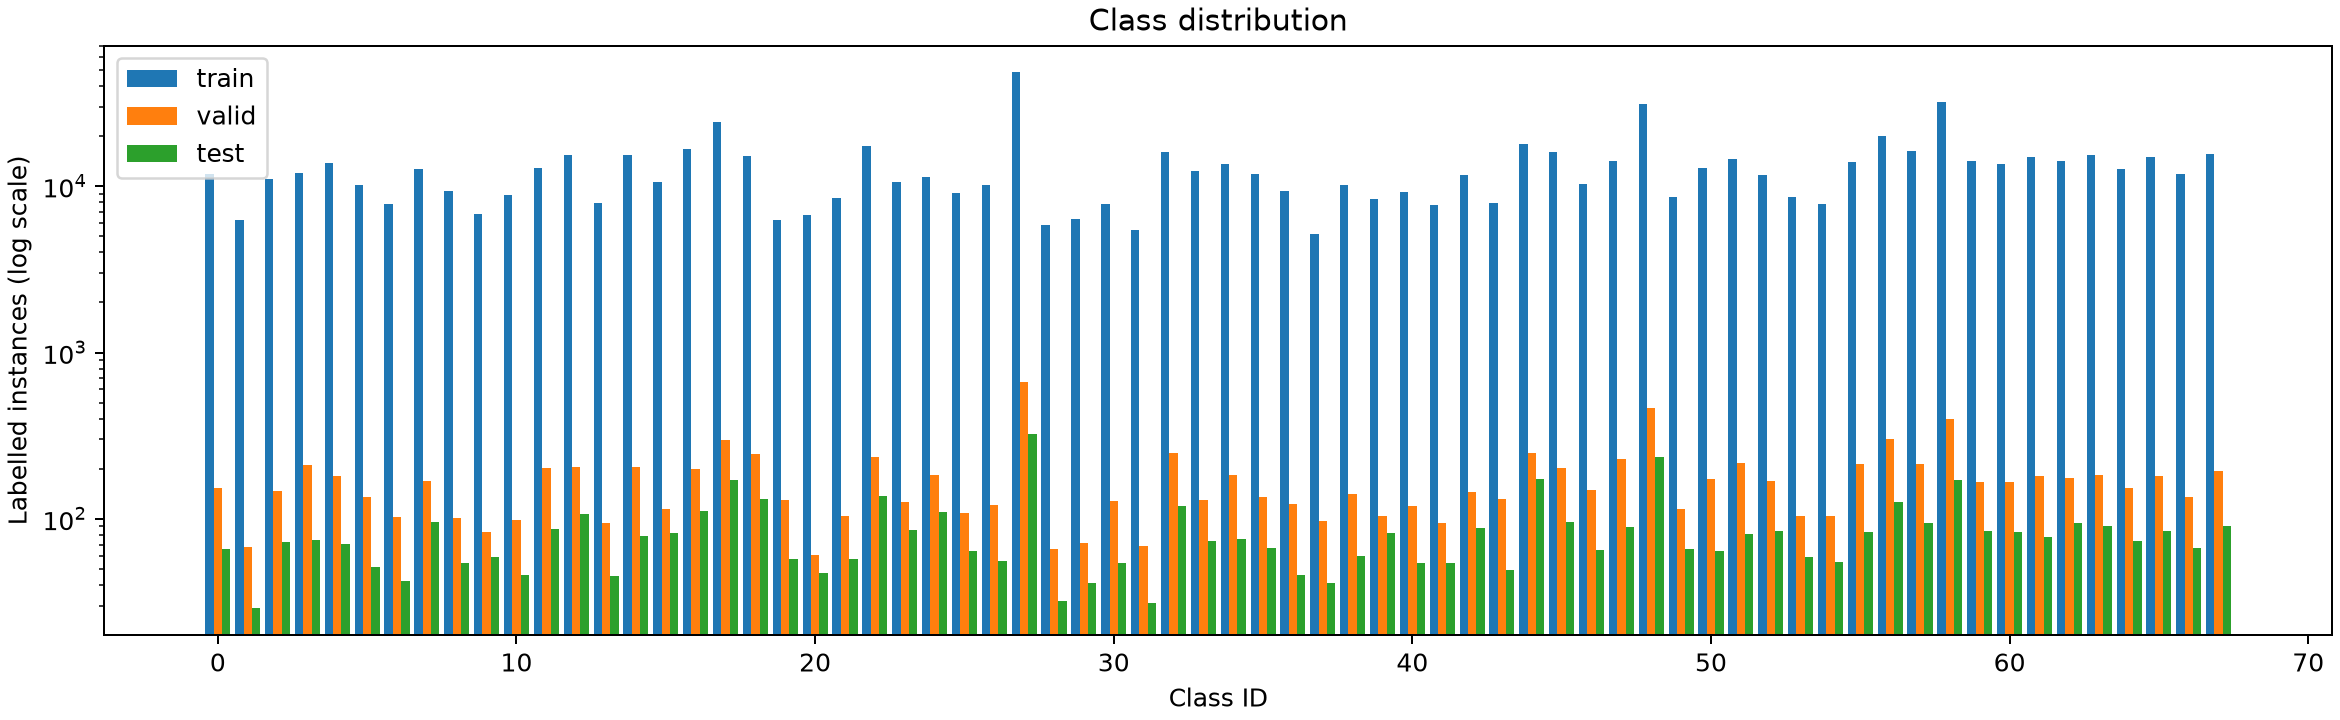
\includegraphics[width=\linewidth,height=0.76\textheight,keepaspectratio]{reports/evaluation/figures/class_distribution.png}
\end{center}

\textbf{Hình 1.} Mỗi cột biểu diễn số hộp, không phải số ảnh; một ảnh có
thể đóng góp cho nhiều lớp.

Số hộp train theo lớp nằm trong khoảng 5.193--48.477, chênh lệch khoảng
9,34 lần. Test chỉ có 29--323 hộp mỗi lớp. Bên cạnh mAP trung bình, cần
theo dõi lớp ít mẫu và lớp có AP thấp; biến động một vài dự đoán có thể
ảnh hưởng lớn đến tỷ lệ của lớp ít mẫu. Số liệu từng lớp được lưu tại
\href{reports/evaluation/dataset_class_counts.csv}{dataset\_class\_counts.csv}.

\section{4. PHƯƠNG PHÁP VÀ TỔ CHỨC HỆ
THỐNG}\label{phux1b0ux1a1ng-phuxe1p-vuxe0-tux1ed5-chux1ee9c-hux1ec7-thux1ed1ng}

\subsection{4.1. Luồng thực
nghiệm}\label{luux1ed3ng-thux1ef1c-nghiux1ec7m}

\begin{center}
\begin{tikzpicture}[every node/.style={draw=blue!55!black,fill=blue!4,rounded corners=2pt,text width=3.25cm,minimum height=1.55cm,align=center,font=\small},>=stealth]
\node (n1) at (0.00,0.00) {Ảnh và nhãn YOLO};
\node (n2) at (3.80,0.00) {Kiểm kê và kiểm tra nhãn};
\node (n3) at (7.60,0.00) {YOLO11s tiền huấn luyện};
\node (n4) at (11.40,0.00) {Train 150 epoch};
\node (n5) at (11.40,-2.20) {Chọn best bằng validation mAP50--95};
\node (n6) at (7.60,-2.20) {Chọn confidence trên validation};
\node (n7) at (3.80,-2.20) {Đánh giá test với mô hình và ngưỡng cố định};
\node (n8) at (0.00,-2.20) {CSV, JSON, biểu đồ và phân tích lỗi};
\draw[->,thick,blue!55!black] (n1) -- (n2);
\draw[->,thick,blue!55!black] (n2) -- (n3);
\draw[->,thick,blue!55!black] (n3) -- (n4);
\draw[->,thick,blue!55!black] (n4) -- (n5);
\draw[->,thick,blue!55!black] (n5) -- (n6);
\draw[->,thick,blue!55!black] (n6) -- (n7);
\draw[->,thick,blue!55!black] (n7) -- (n8);
\end{tikzpicture}
\end{center}

Test chỉ được dùng đánh giá sau khi training hoàn tất. Trong lượt đánh
giá báo cáo, không dùng test để chọn epoch hoặc điều chỉnh trọng số.
Ngưỡng vận hành được chọn từ đường F1 của validation; mAP vẫn được tính
từ dự đoán ở confidence sàn thấp để bảo toàn đường precision--recall.

\subsection{4.2. Tiền xử lý và
augmentation}\label{tiux1ec1n-xux1eed-luxfd-vuxe0-augmentation}

Train dùng ảnh RGB,
\texttt{i\allowbreak{}m\allowbreak{}g\allowbreak{}s\allowbreak{}z\allowbreak{}=\allowbreak{}6\allowbreak{}4\allowbreak{}0\allowbreak{}}
và
\texttt{r\allowbreak{}e\allowbreak{}c\allowbreak{}t\allowbreak{}=\allowbreak{}F\allowbreak{}a\allowbreak{}l\allowbreak{}s\allowbreak{}e\allowbreak{}}.
Thư viện xử lý resize/letterbox và hộp tương ứng. Cấu hình augmentation
thực tế gồm HSV
(\texttt{h\allowbreak{}=\allowbreak{}0\allowbreak{},\allowbreak{}0\allowbreak{}1\allowbreak{}5\allowbreak{}},
\texttt{s\allowbreak{}=\allowbreak{}0\allowbreak{},\allowbreak{}7\allowbreak{}},
\texttt{v\allowbreak{}=\allowbreak{}0\allowbreak{},\allowbreak{}4\allowbreak{}}),
dịch chuyển
\texttt{t\allowbreak{}r\allowbreak{}a\allowbreak{}n\allowbreak{}s\allowbreak{}l\allowbreak{}a\allowbreak{}t\allowbreak{}e\allowbreak{}=\allowbreak{}0\allowbreak{},\allowbreak{}1\allowbreak{}},
thay đổi tỷ lệ
\texttt{s\allowbreak{}c\allowbreak{}a\allowbreak{}l\allowbreak{}e\allowbreak{}=\allowbreak{}0\allowbreak{},\allowbreak{}5\allowbreak{}},
lật ngang
\texttt{f\allowbreak{}l\allowbreak{}i\allowbreak{}p\allowbreak{}l\allowbreak{}r\allowbreak{}=\allowbreak{}0\allowbreak{},\allowbreak{}5\allowbreak{}}
và mosaic với xác suất 1,0 trước giai đoạn đóng mosaic. Xoay, shear,
perspective, lật dọc, mixup, cutmix và copy-paste đặt bằng 0.

\texttt{c\allowbreak{}l\allowbreak{}o\allowbreak{}s\allowbreak{}e\allowbreak{}\_\allowbreak{}m\allowbreak{}o\allowbreak{}s\allowbreak{}a\allowbreak{}i\allowbreak{}c\allowbreak{}=\allowbreak{}1\allowbreak{}0\allowbreak{}}
đóng mosaic trong 10 epoch cuối, từ epoch 141. Hình train tại giai đoạn
này được lưu trong thư mục run. Những trường như
\texttt{a\allowbreak{}u\allowbreak{}t\allowbreak{}o\allowbreak{}\_\allowbreak{}a\allowbreak{}u\allowbreak{}g\allowbreak{}m\allowbreak{}e\allowbreak{}n\allowbreak{}t\allowbreak{}}
và
\texttt{e\allowbreak{}r\allowbreak{}a\allowbreak{}s\allowbreak{}i\allowbreak{}n\allowbreak{}g\allowbreak{}}
có thể xuất hiện trong cấu hình chung của thư viện; báo cáo không coi
chúng là augmentation detection đã áp dụng chỉ vì có trong YAML.

Validation/test không dùng tăng cường dữ liệu lúc đánh giá
(\texttt{a\allowbreak{}u\allowbreak{}g\allowbreak{}m\allowbreak{}e\allowbreak{}n\allowbreak{}t\allowbreak{}=\allowbreak{}F\allowbreak{}a\allowbreak{}l\allowbreak{}s\allowbreak{}e\allowbreak{}}).
Lượt đánh giá dùng
\texttt{r\allowbreak{}e\allowbreak{}c\allowbreak{}t\allowbreak{}=\allowbreak{}T\allowbreak{}r\allowbreak{}u\allowbreak{}e\allowbreak{}}
để ghép theo tỷ lệ ảnh và căn theo stride. Vì vậy
\texttt{i\allowbreak{}m\allowbreak{}g\allowbreak{}s\allowbreak{}z\allowbreak{}=\allowbreak{}6\allowbreak{}4\allowbreak{}0\allowbreak{}}
là kích thước cấu hình, không bảo đảm mọi tensor đều đúng 640×640; hình
vuông có thể được padding lên 672×672 trong evaluator phiên bản đang
dùng. Suy luận benchmark sử dụng
\texttt{r\allowbreak{}e\allowbreak{}c\allowbreak{}t\allowbreak{}=\allowbreak{}F\allowbreak{}a\allowbreak{}l\allowbreak{}s\allowbreak{}e\allowbreak{}},
tensor cố định 640×640.
\href{https://docs.ultralytics.com/modes/val/}{11}

\subsection{4.3. Các thành phần mã
nguồn}\label{cuxe1c-thuxe0nh-phux1ea7n-muxe3-nguux1ed3n}

\begingroup\small\setlength{\tabcolsep}{4pt}\renewcommand{\arraystretch}{1.12}

{\def\LTcaptype{none} % do not increment counter
\begin{longtable}[]{@{}
  >{\raggedright\arraybackslash}p{(\linewidth - 2\tabcolsep) * \real{0.3200}}
  >{\raggedright\arraybackslash}p{(\linewidth - 2\tabcolsep) * \real{0.6800}}@{}}
\toprule\noalign{}
\begin{minipage}[b]{\linewidth}\raggedright
File
\end{minipage} & \begin{minipage}[b]{\linewidth}\raggedright
Vai trò
\end{minipage} \\
\midrule\noalign{}
\endhead
\bottomrule\noalign{}
\endlastfoot
\url{data.yaml} & Đường dẫn ba tập và danh sách ID lớp \\
\url{check_gpu.py} & Kiểm tra CUDA và phép toán có backward \\
\url{train.py} & Tham số train, AMP, AutoBatch, resume và đường dẫn
output \\
\url{memory_trainer.py} & Giới hạn worker/prefetch; validation dùng 0
worker \\
\url{evaluate.py} & Đánh giá validation/test, chọn ngưỡng và lưu số
liệu \\
\url{audit_dataset.py} & Kiểm kê nhãn và trùng ảnh byte \\
\url{analyze_results.py} & Biểu đồ và phân tích lỗi từng ảnh \\
\url{benchmark_inference.py} & Đo suy luận từng ảnh trên mẫu test cố
định \\
\url{render_report.py} & Điền số đo và bảng vào mẫu báo cáo \\
\end{longtable}
}

\endgroup

\section{5. MÔI TRƯỜNG VÀ CẤU HÌNH THỰC
NGHIỆM}\label{muxf4i-trux1b0ux1eddng-vuxe0-cux1ea5u-huxecnh-thux1ef1c-nghiux1ec7m}

\subsection{5.1. Phần cứng và phần
mềm}\label{phux1ea7n-cux1ee9ng-vuxe0-phux1ea7n-mux1ec1m}

\textbf{Bảng 2. Môi trường đo trực tiếp trên máy chạy.}

\begingroup\small\setlength{\tabcolsep}{4pt}\renewcommand{\arraystretch}{1.12}

{\def\LTcaptype{none} % do not increment counter
\begin{longtable}[]{@{}
  >{\raggedright\arraybackslash}p{(\linewidth - 2\tabcolsep) * \real{0.3200}}
  >{\raggedright\arraybackslash}p{(\linewidth - 2\tabcolsep) * \real{0.6800}}@{}}
\toprule\noalign{}
\begin{minipage}[b]{\linewidth}\raggedright
Thành phần
\end{minipage} & \begin{minipage}[b]{\linewidth}\raggedright
Giá trị
\end{minipage} \\
\midrule\noalign{}
\endhead
\bottomrule\noalign{}
\endlastfoot
Hệ điều hành & Windows 11 Pro, build 26200; chạy Windows native \\
GPU & NVIDIA GeForce RTX 5070 desktop, 12 GB \\
CPU & AMD Ryzen 5 7600X3D; 6 lõi vật lý, 12 luồng logic \\
RAM & 32 GB lắp đặt; hệ điều hành báo khoảng 31,11 GiB khả dụng tổng \\
Python & 3.12.13 \\
Ultralytics & 8.4.175 \\
PyTorch / torchvision & 2.8.0+cu128 / 0.23.0+cu128 \\
CUDA runtime của PyTorch & 12.8 \\
Driver NVIDIA & 617.14 \\
OpenCV & 5.0.0.93 \\
Nơi lưu dataset / run & Ổ D; môi trường
\texttt{.\allowbreak{}v\allowbreak{}e\allowbreak{}n\allowbreak{}v\allowbreak{}}
trong repo là junction sang D \\
\end{longtable}
}

\endgroup

CUDA runtime của PyTorch khác phiên bản CUDA tối đa driver hỗ trợ. Không
cần diễn giải số CUDA do
\texttt{n\allowbreak{}v\allowbreak{}i\allowbreak{}d\allowbreak{}i\allowbreak{}a\allowbreak{}-\allowbreak{}s\allowbreak{}m\allowbreak{}i\allowbreak{}}
hiển thị là phiên bản runtime của training. Phiên bản thư viện trước và
sau đánh giá được chụp tại
\href{reports/evaluation/environment-freeze.txt}{environment-freeze.txt}
và
\href{reports/evaluation/environment-freeze-final.txt}{environment-freeze-final.txt}.
Lượt
\texttt{s\allowbreak{}a\allowbreak{}v\allowbreak{}e\allowbreak{}\_\allowbreak{}j\allowbreak{}s\allowbreak{}o\allowbreak{}n\allowbreak{}=\allowbreak{}T\allowbreak{}r\allowbreak{}u\allowbreak{}e\allowbreak{}}
tự bổ sung
\texttt{f\allowbreak{}a\allowbreak{}s\allowbreak{}t\allowbreak{}e\allowbreak{}r\allowbreak{}-\allowbreak{}c\allowbreak{}o\allowbreak{}c\allowbreak{}o\allowbreak{}-\allowbreak{}e\allowbreak{}v\allowbreak{}a\allowbreak{}l\allowbreak{}=\allowbreak{}=\allowbreak{}1\allowbreak{}.\allowbreak{}8\allowbreak{}.\allowbreak{}0\allowbreak{}};
không thay đổi phiên bản PyTorch, Ultralytics hoặc các thư viện training
đang có. Các bảng mAP chính vẫn lấy từ evaluator native, không trộn thêm
chỉ số COCO theo kích thước vật thể.

\subsection{5.2. Cấu hình huấn
luyện}\label{cux1ea5u-huxecnh-huux1ea5n-luyux1ec7n}

\textbf{Bảng 3. Cấu hình cuối được đối chiếu với
\texttt{a\allowbreak{}r\allowbreak{}g\allowbreak{}s\allowbreak{}.\allowbreak{}y\allowbreak{}a\allowbreak{}m\allowbreak{}l\allowbreak{}}
và mã nguồn.}

\begingroup\small\setlength{\tabcolsep}{4pt}\renewcommand{\arraystretch}{1.12}

{\def\LTcaptype{none} % do not increment counter
\begin{longtable}[]{@{}
  >{\raggedright\arraybackslash}p{(\linewidth - 2\tabcolsep) * \real{0.3200}}
  >{\raggedright\arraybackslash}p{(\linewidth - 2\tabcolsep) * \real{0.6800}}@{}}
\toprule\noalign{}
\begin{minipage}[b]{\linewidth}\raggedright
Tham số
\end{minipage} & \begin{minipage}[b]{\linewidth}\raggedright
Cấu hình thực nghiệm
\end{minipage} \\
\midrule\noalign{}
\endhead
\bottomrule\noalign{}
\endlastfoot
Model / khởi tạo & YOLO11s /
\texttt{y\allowbreak{}o\allowbreak{}l\allowbreak{}o\allowbreak{}1\allowbreak{}1\allowbreak{}s\allowbreak{}.\allowbreak{}p\allowbreak{}t\allowbreak{}}
tiền huấn luyện \\
Số lớp & 68 \\
Epoch & 150; hoàn tất đủ 150 \\
Kích thước train & 640×640,
\texttt{r\allowbreak{}e\allowbreak{}c\allowbreak{}t\allowbreak{}=\allowbreak{}F\allowbreak{}a\allowbreak{}l\allowbreak{}s\allowbreak{}e\allowbreak{}} \\
Batch & 28 ở giai đoạn đầu; 36 từ epoch 73 \\
Train workers / prefetch cuối & 4 worker / 2 batch mỗi worker \\
Validation workers trong train & 0, do trainer tùy chỉnh \\
Image cache & Tắt
(\texttt{c\allowbreak{}a\allowbreak{}c\allowbreak{}h\allowbreak{}e\allowbreak{}=\allowbreak{}F\allowbreak{}a\allowbreak{}l\allowbreak{}s\allowbreak{}e\allowbreak{}}) \\
Device / AMP & CUDA:0 / bật \\
Optimizer thực tế & MuSGD, được chọn từ chế độ
\texttt{a\allowbreak{}u\allowbreak{}t\allowbreak{}o\allowbreak{}} \\
\texttt{l\allowbreak{}r\allowbreak{}0\allowbreak{}},
\texttt{l\allowbreak{}r\allowbreak{}f\allowbreak{}}, momentum & 0,01;
0,01; 0,937 trong cấu hình lưu \\
Weight decay / warmup & 0,0005 / 3 epoch \\
Lịch learning rate & Cosine
(\texttt{c\allowbreak{}o\allowbreak{}s\allowbreak{}\_\allowbreak{}l\allowbreak{}r\allowbreak{}=\allowbreak{}T\allowbreak{}r\allowbreak{}u\allowbreak{}e\allowbreak{}}) \\
\texttt{n\allowbreak{}b\allowbreak{}s\allowbreak{}} & 64; batch thực có
thể kết hợp gradient accumulation \\
Seed / deterministic & 42 / False \\
Early stopping &
\texttt{p\allowbreak{}a\allowbreak{}t\allowbreak{}i\allowbreak{}e\allowbreak{}n\allowbreak{}c\allowbreak{}e\allowbreak{}=\allowbreak{}3\allowbreak{}0\allowbreak{}} \\
Đóng mosaic & 10 epoch cuối \\
Lưu định kỳ &
\texttt{s\allowbreak{}a\allowbreak{}v\allowbreak{}e\allowbreak{}\_\allowbreak{}p\allowbreak{}e\allowbreak{}r\allowbreak{}i\allowbreak{}o\allowbreak{}d\allowbreak{}=\allowbreak{}1\allowbreak{}0\allowbreak{}};
ngoài
\texttt{b\allowbreak{}e\allowbreak{}s\allowbreak{}t\allowbreak{}.\allowbreak{}p\allowbreak{}t\allowbreak{}}
và
\texttt{l\allowbreak{}a\allowbreak{}s\allowbreak{}t\allowbreak{}.\allowbreak{}p\allowbreak{}t\allowbreak{}} \\
\end{longtable}
}

\endgroup

MuSGD được ghi trong cấu hình cuối, không thay bằng AdamW khi mô tả. Chế
độ \texttt{a\allowbreak{}u\allowbreak{}t\allowbreak{}o\allowbreak{}} của
thư viện có thể tự chọn optimizer và learning rate; các giá trị cấu hình
không thay thế việc kiểm tra log learning rate thực tế. Cột
\texttt{l\allowbreak{}r\allowbreak{}/\allowbreak{}p\allowbreak{}g\allowbreak{}*\allowbreak{}}
đã được lưu trong
\texttt{r\allowbreak{}e\allowbreak{}s\allowbreak{}u\allowbreak{}l\allowbreak{}t\allowbreak{}s\allowbreak{}.\allowbreak{}c\allowbreak{}s\allowbreak{}v\allowbreak{}}.
\href{https://docs.ultralytics.com/modes/train/}{12}

\texttt{n\allowbreak{}b\allowbreak{}s\allowbreak{}=\allowbreak{}6\allowbreak{}4\allowbreak{}}
không có nghĩa batch vật lý luôn 64. Với quy tắc tích lũy của phiên bản
đang dùng, batch 28 cho khoảng 56 ảnh mỗi bước cập nhật sau warmup,
batch 36 cho khoảng 72. Thay batch có thể thay đổi đường tối ưu. Vì các
thay đổi xảy ra trong cùng run, không thể quy toàn bộ mức tăng precision
cho batch lớn hơn.

\subsection{5.3. Tối ưu bộ nhớ và lưu
trữ}\label{tux1ed1i-ux1b0u-bux1ed9-nhux1edb-vuxe0-lux1b0u-trux1eef}

Trong quá trình chạy, máy từng có RAM dùng khoảng 30,4 GB và committed
memory 61,5/62,5 GB. Lỗi OpenCV báo không cấp phát được khoảng 6,2 MB
xảy ra ở DataLoader worker; đây là tình trạng bộ nhớ hệ thống, không
phải chỉ nhìn VRAM để chẩn đoán.

DataLoader worker chuẩn bị ảnh ở phía CPU; nhiều worker và hàng đợi
prefetch làm nhiều batch tồn tại đồng thời. Trên Windows, các tiến trình
có thể giữ bản sao cấu trúc dataset; train và validation có thể cùng giữ
pool. Tài liệu PyTorch mô tả rõ mối liên hệ worker, prefetch và bộ nhớ
tiến trình. \href{https://docs.pytorch.org/docs/2.8/data.html}{13}

Giải pháp áp dụng trong repo: tắt cache ảnh RAM, giảm/kiểm soát
prefetch, giữ validation 0 worker và tăng train worker từng bước. Hồ sơ
cuối có 4×2=8 batch prefetch danh nghĩa, ngoài batch đang xử lý và các
buffer khác. AMP được bật để giảm một phần chi phí tính toán/bộ nhớ GPU;
AMP không giới hạn tổng RAM của worker.
\href{https://docs.pytorch.org/docs/2.8/amp.html}{14}

Dataset, run và môi trường Python được chuyển sang D. Tuy nhiên, chuyển
output không đồng nghĩa mọi file hệ thống chuyển theo: pagefile và một
số thư mục tạm vẫn có thể dùng C. Báo cáo không xác nhận đã di chuyển
pagefile. Cần theo dõi RAM committed và dung lượng C cùng GPU memory.

\subsection{5.4. Thời gian và các lần tiếp tục
train}\label{thux1eddi-gian-vuxe0-cuxe1c-lux1ea7n-tiux1ebfp-tux1ee5c-train}

CSV có đủ 150 epoch nhưng cột
\texttt{t\allowbreak{}i\allowbreak{}m\allowbreak{}e\allowbreak{}} bị đặt
lại ở các lần resume. Không dùng giá trị
\texttt{t\allowbreak{}i\allowbreak{}m\allowbreak{}e\allowbreak{}} cuối
như tổng thời gian chạy từ đầu và không cộng mù mọi chênh lệch âm/dương.
Trong đoạn ổn định \textbf{epoch 74--150}, chênh lệch thời gian giữa hai
dòng liên tiếp có trung vị \textbf{13,36 phút/epoch}, khoảng
\textbf{13,29--13,72 phút}. Đây là thời gian vòng epoch ghi trong CSV,
có phần validation và thao tác cuối epoch.

Nếu giữ tốc độ trung vị này từ đầu, 150 epoch tương đương khoảng
\textbf{33,40 giờ}. Con số này là ước lượng theo tốc độ của đoạn ổn
định, không phải tổng thời gian thực tế đã đo cho run có gián đoạn. Chưa
có nhật ký đầy đủ để tổng hợp thời gian nghỉ, lần chạy dở và mọi lần
restart.

Early stopping theo
\texttt{p\allowbreak{}a\allowbreak{}t\allowbreak{}i\allowbreak{}e\allowbreak{}n\allowbreak{}c\allowbreak{}e\allowbreak{}=\allowbreak{}3\allowbreak{}0\allowbreak{}}
sẽ dừng khi tiêu chí theo dõi không cải thiện đủ lâu. Run này kết thúc
do đạt 150 epoch, không dừng sớm. Sau kết thúc bình thường, checkpoint
đã được strip optimizer; không dùng
\texttt{r\allowbreak{}e\allowbreak{}s\allowbreak{}u\allowbreak{}m\allowbreak{}e\allowbreak{}=\allowbreak{}T\allowbreak{}r\allowbreak{}u\allowbreak{}e\allowbreak{}}
để tiếp tục trạng thái tối ưu đã bị loại khỏi
\texttt{b\allowbreak{}e\allowbreak{}s\allowbreak{}t\allowbreak{}.\allowbreak{}p\allowbreak{}t\allowbreak{}}/\texttt{l\allowbreak{}a\allowbreak{}s\allowbreak{}t\allowbreak{}.\allowbreak{}p\allowbreak{}t\allowbreak{}}
hiện tại.

\section{6. QUY TRÌNH ĐÁNH GIÁ}\label{quy-truxecnh-ux111uxe1nh-giuxe1}

\subsection{6.1. Chọn mô hình và
ngưỡng}\label{chux1ecdn-muxf4-huxecnh-vuxe0-ngux1b0ux1ee1ng}

\begin{enumerate}
\def\labelenumi{\arabic{enumi}.}
\tightlist
\item
  Chọn
  \texttt{b\allowbreak{}e\allowbreak{}s\allowbreak{}t\allowbreak{}.\allowbreak{}p\allowbreak{}t\allowbreak{}}
  theo fitness validation của phiên bản đang dùng. Kiểm tra mã
  \texttt{M\allowbreak{}e\allowbreak{}t\allowbreak{}r\allowbreak{}i\allowbreak{}c\allowbreak{}.\allowbreak{}f\allowbreak{}i\allowbreak{}t\allowbreak{}n\allowbreak{}e\allowbreak{}s\allowbreak{}s\allowbreak{}}
  cho trọng số
  \texttt{[\allowbreak{}0\allowbreak{},\allowbreak{}0\allowbreak{},\allowbreak{}0\allowbreak{},\allowbreak{}1\allowbreak{}]\allowbreak{}}
  với thứ tự P, R, mAP50, mAP50--95, nên tiêu chí chọn là mAP50--95.
\item
  Đọc toàn bộ CSV: epoch 150 có mAP50--95 cao nhất. Không chọn
  checkpoint bằng kết quả test.
\item
  Đánh giá lại best trên toàn bộ validation; chọn confidence
  \textbf{0,5936} tại cực đại của đường F1 trung bình đã làm trơn theo
  evaluator.
\item
  Đánh giá test với cùng trọng số và cấu hình. Giữ confidence đã chọn
  trên validation khi báo cáo điểm vận hành.
\end{enumerate}

Evaluator native vẫn xuất P/R ở confidence tối ưu F1 riêng của mỗi tập.
Ngưỡng native của test là \textbf{0,5676}, chỉ dùng diễn giải bảng mặc
định. Báo cáo đồng thời cung cấp điểm vận hành đã khóa theo validation
để tránh trình bày việc tối ưu ngưỡng trên test như kết quả triển khai.

\subsection{6.2. Cấu hình evaluator}\label{cux1ea5u-huxecnh-evaluator}

\begingroup\small\setlength{\tabcolsep}{4pt}\renewcommand{\arraystretch}{1.12}

{\def\LTcaptype{none} % do not increment counter
\begin{longtable}[]{@{}
  >{\raggedright\arraybackslash}p{(\linewidth - 2\tabcolsep) * \real{0.3200}}
  >{\raggedright\arraybackslash}p{(\linewidth - 2\tabcolsep) * \real{0.6800}}@{}}
\toprule\noalign{}
\begin{minipage}[b]{\linewidth}\raggedright
Tham số
\end{minipage} & \begin{minipage}[b]{\linewidth}\raggedright
Giá trị
\end{minipage} \\
\midrule\noalign{}
\endhead
\bottomrule\noalign{}
\endlastfoot
Dữ liệu & Toàn bộ validation 6.602 ảnh; toàn bộ test 3.284 ảnh \\
\texttt{i\allowbreak{}m\allowbreak{}g\allowbreak{}s\allowbreak{}z\allowbreak{}},
\texttt{r\allowbreak{}e\allowbreak{}c\allowbreak{}t\allowbreak{}} & 640,
True \\
Batch / workers & 16 / 0 \\
Kiểu tính toán & FP16 trên CUDA:0 \\
Confidence sàn khi tính AP & 0,001 \\
NMS IoU & 0,70 \\
IoU ghép cặp cho AP & 0,50:0,05:0,95 \\
\texttt{m\allowbreak{}a\allowbreak{}x\allowbreak{}\_\allowbreak{}d\allowbreak{}e\allowbreak{}t\allowbreak{}}
& 300 \\
Test-time augmentation & Tắt \\
Output & Đường P/R/F1, confusion matrix, predictions JSON, CSV từng
lớp \\
\end{longtable}
}

\endgroup

NMS IoU 0,70 và IoU ghép cặp 0,50 có hai vai trò khác nhau. Không dùng
0,70 để diễn giải điều kiện TP trong bảng TP/FP/FN. Tham số
\texttt{h\allowbreak{}a\allowbreak{}l\allowbreak{}f\allowbreak{}=\allowbreak{}T\allowbreak{}r\allowbreak{}u\allowbreak{}e\allowbreak{}}
được thư viện chuyển sang FP16; phiên bản hiện tại cảnh báo tên tham số
này sắp thay bằng
\texttt{q\allowbreak{}u\allowbreak{}a\allowbreak{}n\allowbreak{}t\allowbreak{}i\allowbreak{}z\allowbreak{}e\allowbreak{}=\allowbreak{}1\allowbreak{}6\allowbreak{}},
nhưng lượt đánh giá đã hoàn thành bình thường.

Script giữ lại thống kê ghép cặp trước khi Ultralytics xóa chúng. Một
lượt phân tích độc lập sau đó đọc predictions JSON, lọc theo confidence
validation rồi ghép lại với nhãn gốc trên tọa độ ảnh. Các số TP/FP/FN
trùng với phép đếm từ evaluator, giúp kiểm tra điểm vận hành. JSON làm
tròn bbox đến 3 chữ số thập phân và score đến 5 chữ số; các trường hợp
sát ngưỡng cần lưu ý sai số làm tròn.

\subsection{6.3. Quy tắc đọc confusion
matrix}\label{quy-tux1eafc-ux111ux1ecdc-confusion-matrix}

Ma trận mặc định của lượt val/test dùng confidence sàn \textbf{0,001} và
IoU hình học \textbf{0,45}, nên không đại diện trực tiếp cho ngưỡng
triển khai. Báo cáo tạo thêm ma trận tại \textbf{confidence 0,5936, IoU
0,50}. Hàng là lớp dự đoán, cột là GT; hàng/cột cuối biểu diễn
background/bỏ sót.

Ghép cặp hình học của confusion matrix không bắt buộc cùng lớp trước khi
ghép; cách ghép của AP có điều kiện cùng lớp. Do đó không bắt buộc tổng
đường chéo của matrix bằng TP từ AP trong mọi trường hợp có hộp chồng
nhau. Không lấy matrix mặc định để suy lại P/R ở confidence khác.

\section{7. KẾT QUẢ VÀ THẢO
LUẬN}\label{kux1ebft-quux1ea3-vuxe0-thux1ea3o-luux1eadn}

\subsection{7.1. Diễn biến huấn
luyện}\label{diux1ec5n-biux1ebfn-huux1ea5n-luyux1ec7n}

\begin{center}
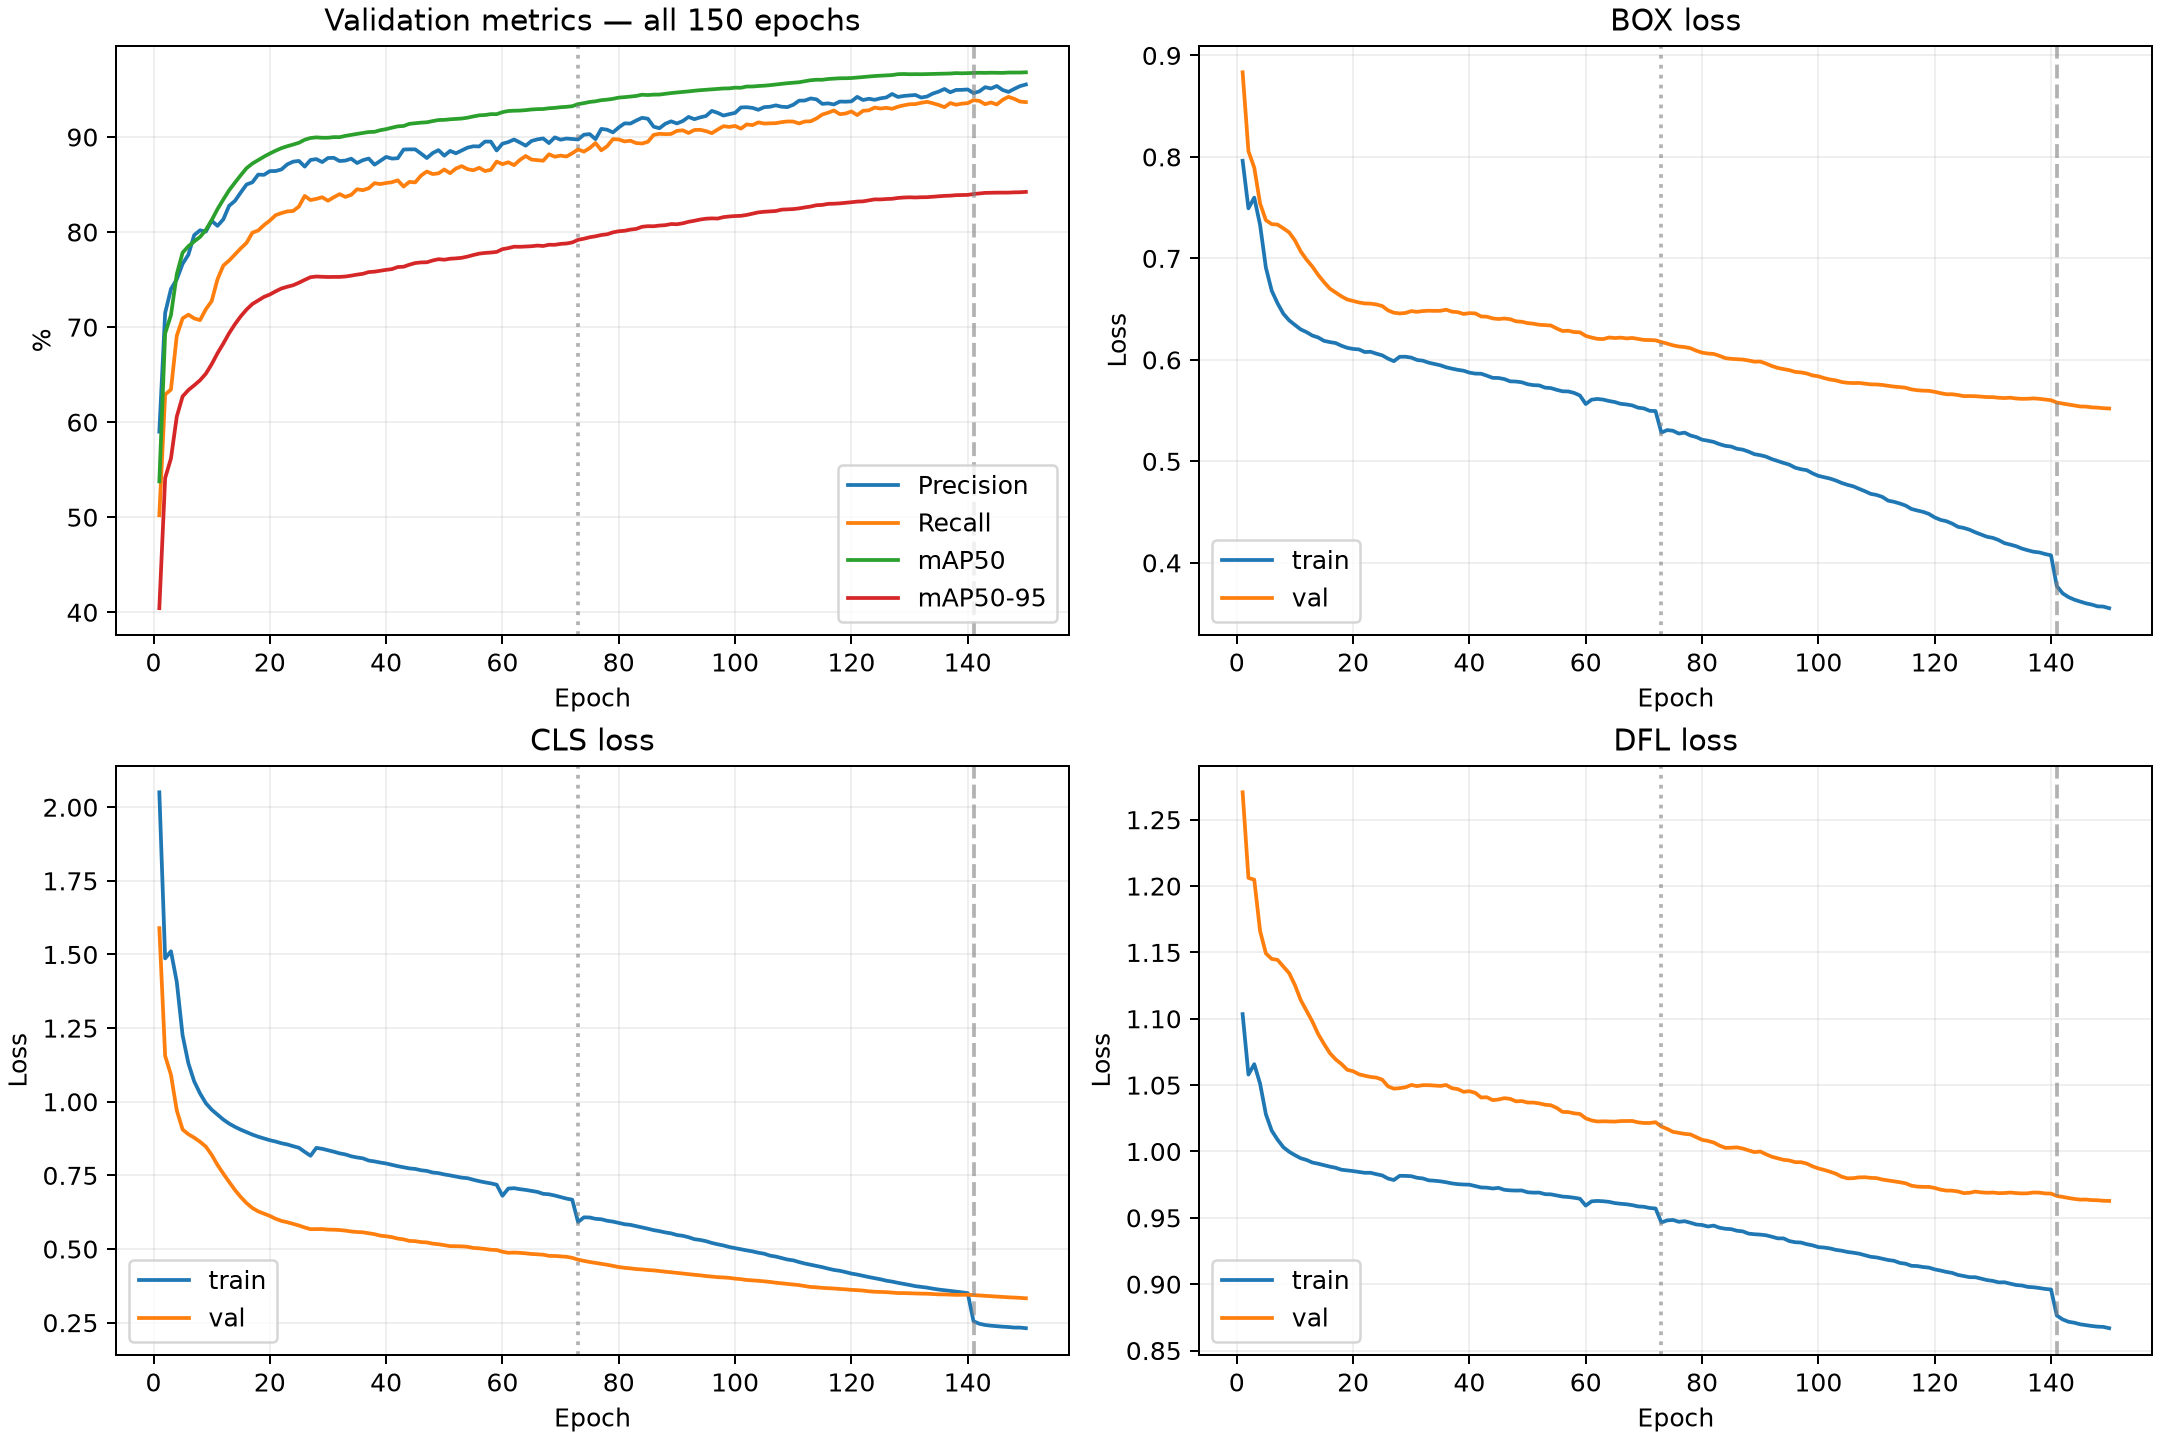
\includegraphics[width=\linewidth,height=0.76\textheight,keepaspectratio]{reports/evaluation/figures/training_curves_150.png}
\end{center}

\textbf{Hình 2.} Vạch chấm tại epoch 73 đánh dấu batch 36; vạch đứt tại
epoch 141 đánh dấu đóng mosaic. Các mốc biểu diễn thay đổi cấu hình,
không chứng minh tác động nhân quả của chúng.

\textbf{Bảng 4. Một số mốc từ log huấn luyện; chỉ số đều tính trên
validation.}

\begingroup\small\setlength{\tabcolsep}{4pt}\renewcommand{\arraystretch}{1.12}

{\def\LTcaptype{none} % do not increment counter
\begin{longtable}[]{@{}lllll@{}}
\toprule\noalign{}
Epoch & Precision & Recall & mAP50 & mAP50--95 \\
\midrule\noalign{}
\endhead
\bottomrule\noalign{}
\endlastfoot
1 & 59,00 & 50,20 & 53,77 & 40,43 \\
10 & 81,19 & 72,73 & 81,25 & 66,10 \\
25 & 87,49 & 82,69 & 89,39 & 74,67 \\
50 & 88,03 & 86,58 & 91,81 & 77,09 \\
72 & 89,79 & 88,30 & 93,24 & 78,91 \\
73 & 89,74 & 88,69 & 93,46 & 79,18 \\
100 & 92,54 & 91,17 & 95,19 & 81,69 \\
125 & 94,07 & 93,00 & 96,45 & 83,43 \\
140 & 95,00 & 93,56 & 96,73 & 83,91 \\
141 & 94,62 & 93,88 & 96,75 & 84,00 \\
150 & 95,53 & 93,67 & 96,81 & 84,23 \\
\end{longtable}
}

\endgroup

Từ epoch 1 đến 150, precision tăng \textbf{36,53 điểm phần trăm}, recall
tăng \textbf{43,47 điểm} và mAP50--95 tăng \textbf{43,80 điểm}.
Precision có dao động cục bộ; giảm ở một epoch không đủ kết luận mô hình
suy giảm dài hạn. Ở giai đoạn cuối, chỉ số vẫn cải thiện nhưng mức tăng
nhỏ dần.

Epoch 150 có train box/cls/DFL loss lần lượt \textbf{0,35527 / 0,23118 /
0,86684}; validation tương ứng \textbf{0,55206 / 0,33274 / 0,96275}. Val
box loss và cls loss tiếp tục giảm cùng mAP tăng, nên chưa thấy dấu hiệu
suy giảm validation kéo dài trong run này. Tuy nhiên, chưa kiểm chứng
nguồn chia tập, chưa có nhiều seed hoặc tập ngoài miền để loại trừ
overfitting hay ước lượng bất định.

\subsection{7.2. Kết quả tổng
thể}\label{kux1ebft-quux1ea3-tux1ed5ng-thux1ec3}

\textbf{Bảng 5. So sánh log cuối, đánh giá lại validation và test. Đơn
vị chỉ số: \%.}

\begingroup\small\setlength{\tabcolsep}{4pt}\renewcommand{\arraystretch}{1.12}

{\def\LTcaptype{none} % do not increment counter
\begin{longtable}[]{@{}llllll@{}}
\toprule\noalign{}
Nguồn & Ảnh & Precision & Recall & mAP50 & mAP50--95 \\
\midrule\noalign{}
\endhead
\bottomrule\noalign{}
\endlastfoot
Log epoch 150 (validation) & 6.602 & 95,53 & 93,67 & 96,81 & 84,23 \\
Validation đánh giá lại & 6.602 & 95,58 & 93,66 & 96,80 & 84,22 \\
Test sau training & 3.284 & 95,34 & 94,54 & 97,23 & 85,32 \\
\end{longtable}
}

\endgroup

Số validation đánh giá lại có chênh lệch nhỏ với log cuối do điều kiện
evaluator như batch và tính toán FP16; mức chênh lệch không làm thay đổi
kết luận về run. Test có mAP50--95 cao hơn validation khoảng
\textbf{1,09 điểm phần trăm}. Không diễn giải điều đó là test tốt hơn
mọi tình huống thực tế; độ khó, phân bố đối tượng và mẫu của từng tập có
thể khác nhau.

Kết quả test 95,34\% precision cho thấy mục tiêu trên 95\% đã đạt theo
\textbf{cách tổng hợp native của evaluator}. Đây không phải tỷ lệ ảnh
nhận diện đúng hoàn toàn, không phải precision của mọi lớp, và không
phải bảo đảm cho ảnh mới ngoài bộ dữ liệu.

\subsection{7.3. Ảnh hưởng ngưỡng
confidence}\label{ux1ea3nh-hux1b0ux1edfng-ngux1b0ux1ee1ng-confidence}

\textbf{Bảng 6. TP/FP/FN test ở IoU 0,50; P/R là micro.}

\begingroup\small\setlength{\tabcolsep}{4pt}\renewcommand{\arraystretch}{1.12}

{\def\LTcaptype{none} % do not increment counter
\begin{longtable}[]{@{}llllll@{}}
\toprule\noalign{}
Confidence & TP & FP & FN & Precision micro & Recall micro \\
\midrule\noalign{}
\endhead
\bottomrule\noalign{}
\endlastfoot
0,2500 & 5455 & 508 & 215 & 91,48 & 96,21 \\
0,5936 & 5316 & 222 & 354 & 95,99 & 93,76 \\
\end{longtable}
}

\endgroup

Ngưỡng khóa theo validation giảm FP từ 508 xuống 222 so với 0,25, đồng
thời tăng FN từ 215 lên 354. Mức đánh đổi này phù hợp khi ưu tiên ít
phát hiện sai; hệ thống cần quan sát đầy đủ thành phần có thể chọn
ngưỡng thấp hơn và chấp nhận thêm FP. Việc lựa chọn phải xuất phát từ
mục tiêu ứng dụng và validation.

Ở confidence 0,5936, \textbf{macro precision 96,10\% và macro recall
93,94\%} từ số đếm theo lớp; micro tương ứng 95,99\% và 93,76\%. Native
P/R có nội suy trên đường confidence nên có thể khác một chút số đếm
trực tiếp tại một ngưỡng. Không trộn hai cách tính để kết luận tăng/giảm
chất lượng.

\begin{center}
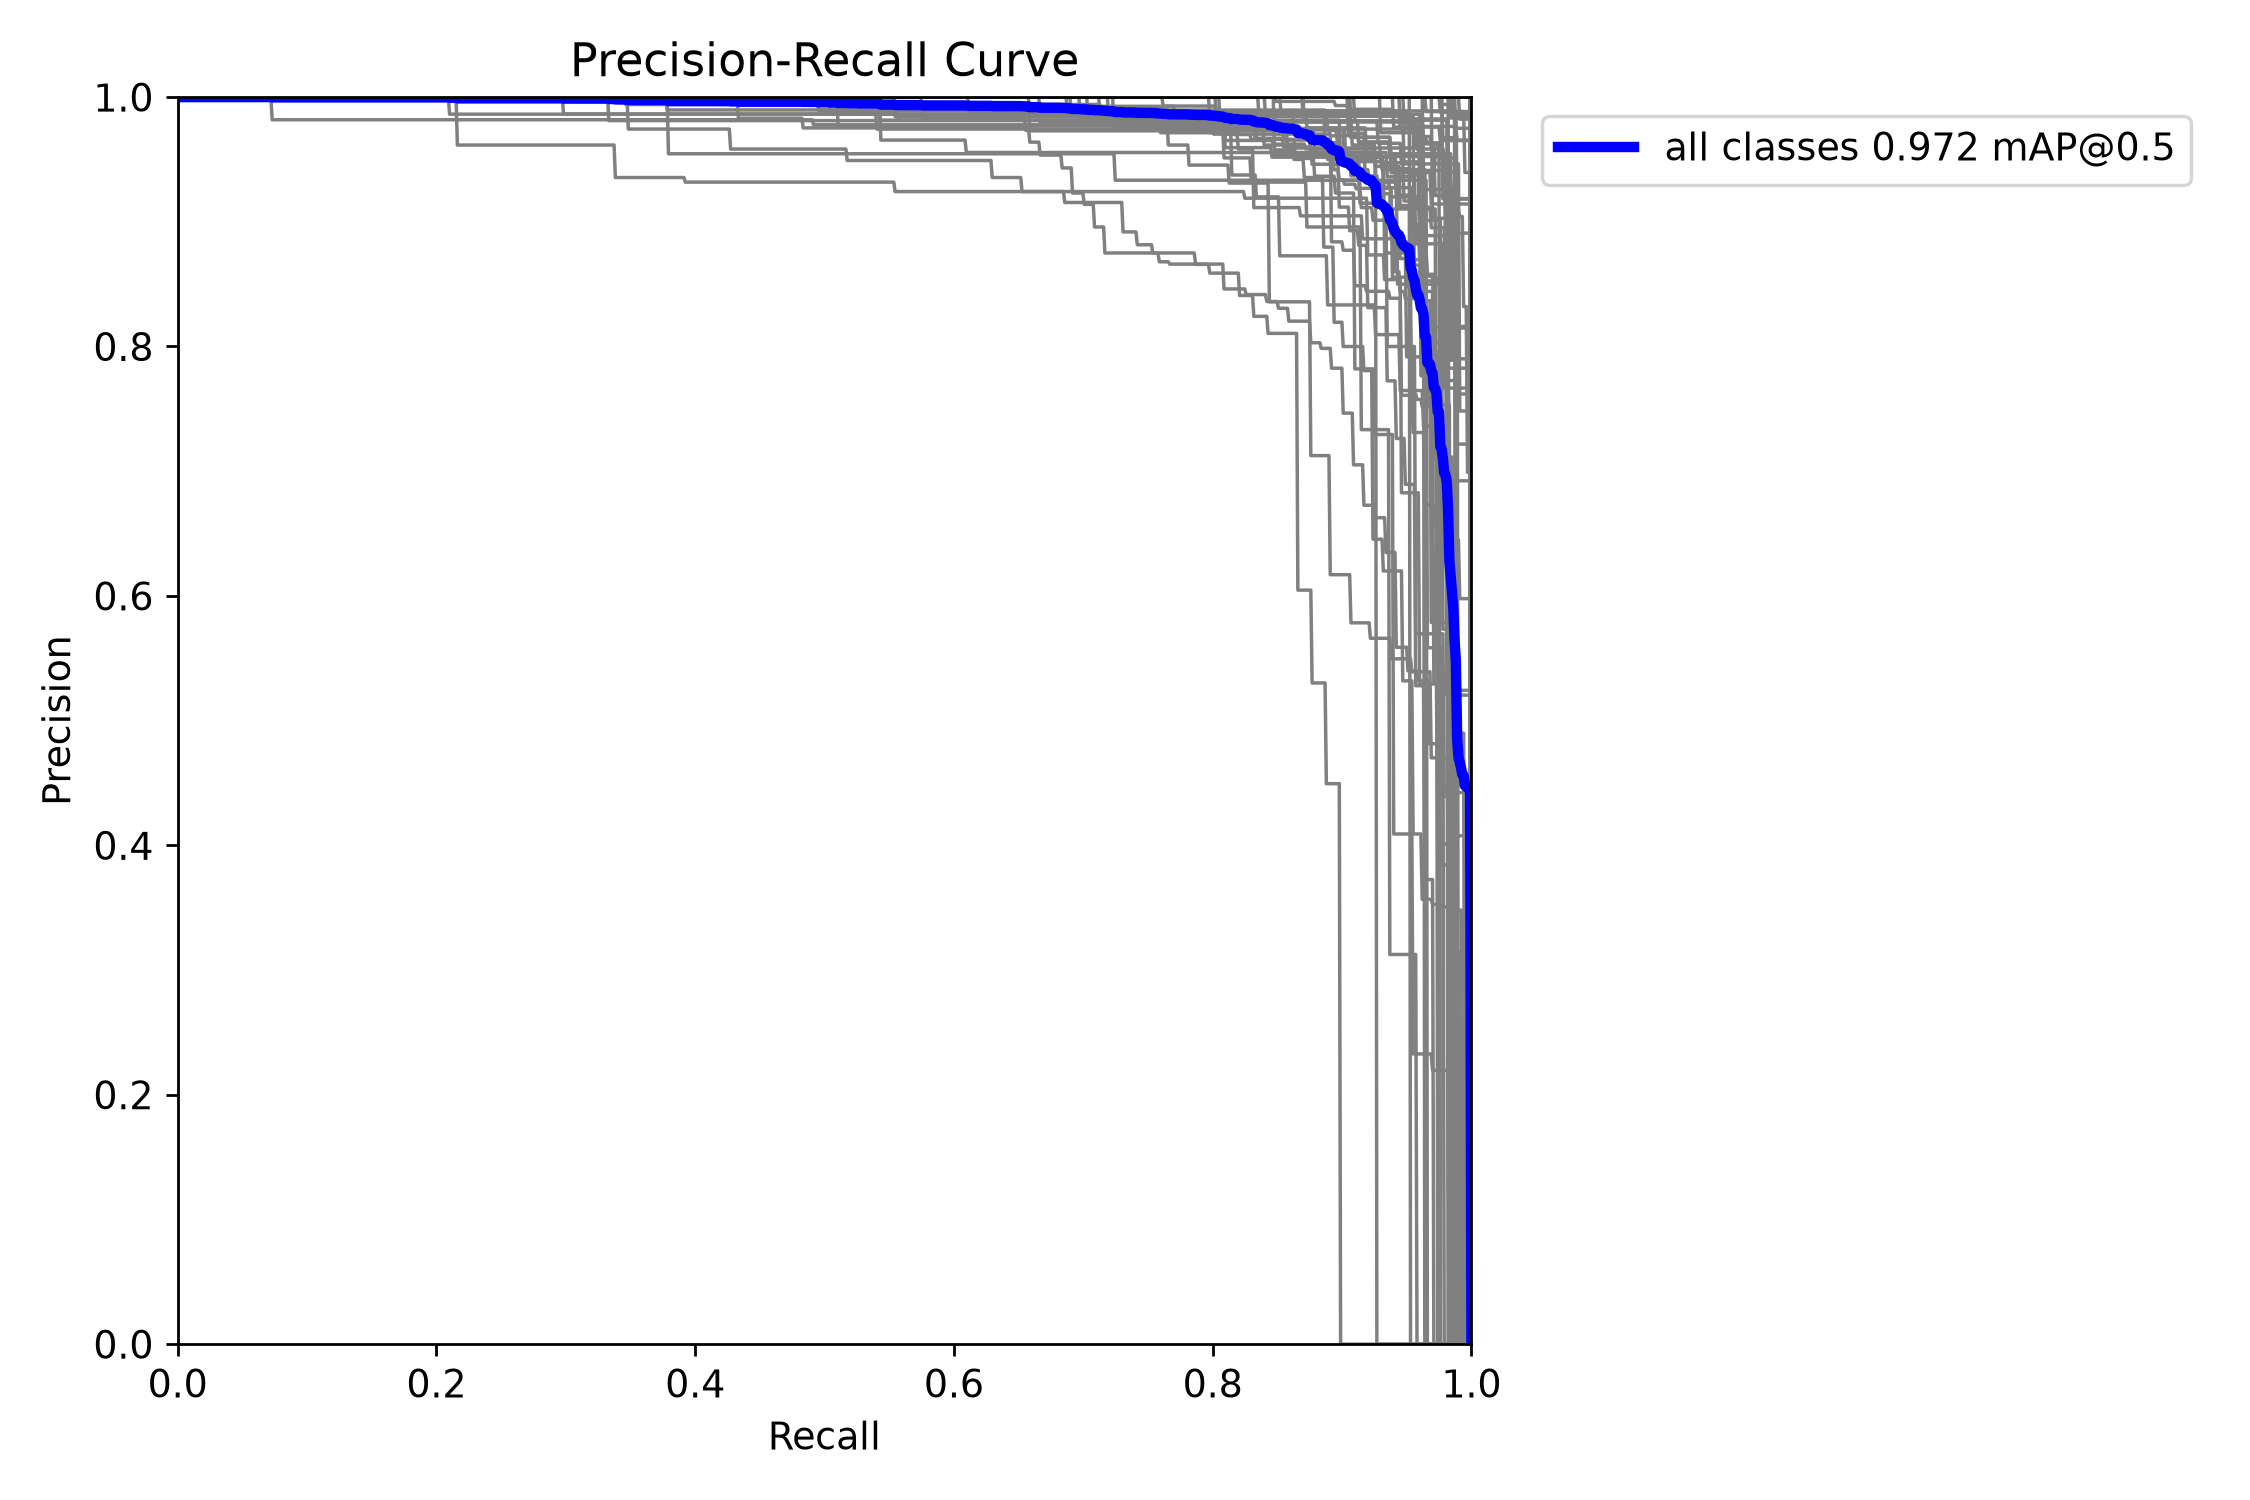
\includegraphics[width=\linewidth,height=0.76\textheight,keepaspectratio]{reports/evaluation/figures/test_BoxPR_curve.png}
\end{center}

\textbf{Hình 3.} Đường từng lớp và đường trung bình từ evaluator, sử
dụng confidence sàn 0,001. Hình hỗ trợ quan sát đánh đổi
precision--recall; không dùng đường test để lựa chọn ngưỡng triển khai.

\subsection{7.4. Kết quả từng
lớp}\label{kux1ebft-quux1ea3-tux1eebng-lux1edbp}

\begin{center}
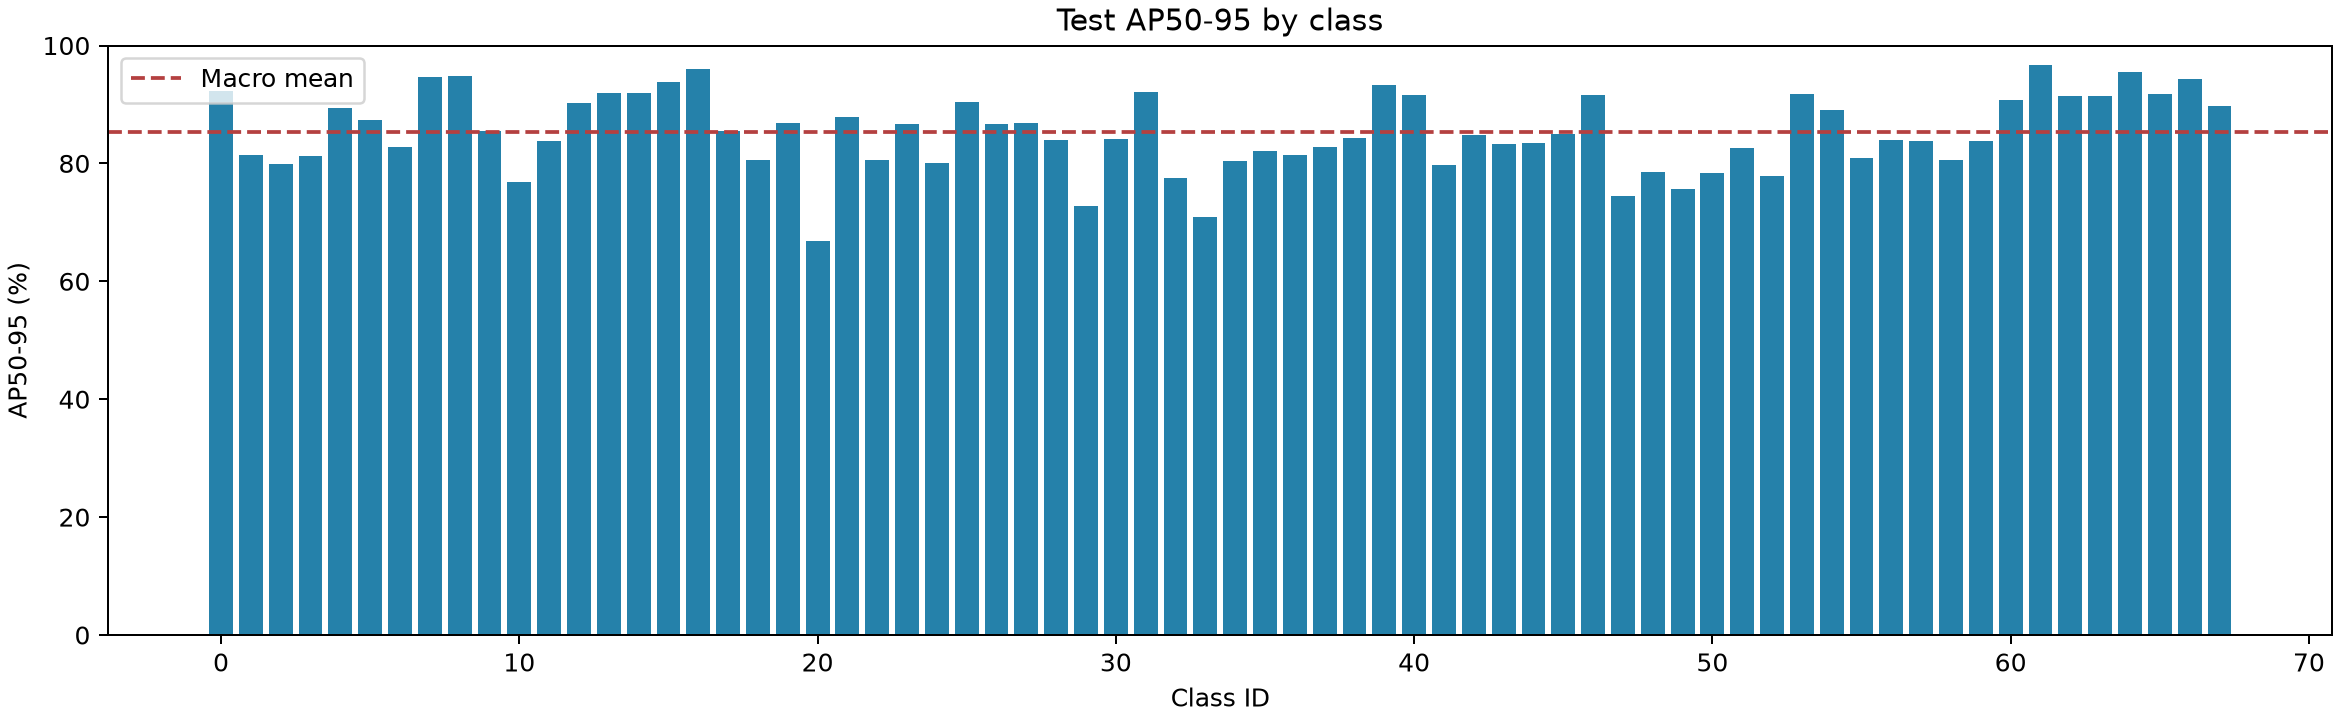
\includegraphics[width=\linewidth,height=0.76\textheight,keepaspectratio]{reports/evaluation/figures/test_ap_by_class.png}
\end{center}

\textbf{Bảng 7. Năm lớp có AP50--95 test thấp nhất; tên vẫn dùng ID cục
bộ.}

\begingroup\small\setlength{\tabcolsep}{4pt}\renewcommand{\arraystretch}{1.12}

{\def\LTcaptype{none} % do not increment counter
\begin{longtable}[]{@{}
  >{\raggedright\arraybackslash}p{(\linewidth - 12\tabcolsep) * \real{0.1900}}
  >{\raggedright\arraybackslash}p{(\linewidth - 12\tabcolsep) * \real{0.1350}}
  >{\raggedright\arraybackslash}p{(\linewidth - 12\tabcolsep) * \real{0.1350}}
  >{\raggedright\arraybackslash}p{(\linewidth - 12\tabcolsep) * \real{0.1150}}
  >{\raggedright\arraybackslash}p{(\linewidth - 12\tabcolsep) * \real{0.1150}}
  >{\raggedright\arraybackslash}p{(\linewidth - 12\tabcolsep) * \real{0.1000}}
  >{\raggedright\arraybackslash}p{(\linewidth - 12\tabcolsep) * \real{0.2100}}@{}}
\toprule\noalign{}
\begin{minipage}[b]{\linewidth}\raggedright
Lớp
\end{minipage} & \begin{minipage}[b]{\linewidth}\raggedright
Ảnh có GT
\end{minipage} & \begin{minipage}[b]{\linewidth}\raggedright
Hộp GT
\end{minipage} & \begin{minipage}[b]{\linewidth}\raggedright
P
\end{minipage} & \begin{minipage}[b]{\linewidth}\raggedright
R
\end{minipage} & \begin{minipage}[b]{\linewidth}\raggedright
AP50
\end{minipage} & \begin{minipage}[b]{\linewidth}\raggedright
AP50--95
\end{minipage} \\
\midrule\noalign{}
\endhead
\bottomrule\noalign{}
\endlastfoot
class\_20 & 25 & 47 & 92,72 & 87,23 & 92,53 & 66,80 \\
class\_33 & 49 & 74 & 89,79 & 91,89 & 91,53 & 70,94 \\
class\_29 & 37 & 41 & 96,66 & 90,24 & 92,14 & 72,84 \\
class\_47 & 43 & 89 & 85,87 & 81,93 & 84,23 & 74,53 \\
class\_49 & 53 & 66 & 92,20 & 89,57 & 93,68 & 75,68 \\
\end{longtable}
}

\endgroup

Lớp
\texttt{c\allowbreak{}l\allowbreak{}a\allowbreak{}s\allowbreak{}s\allowbreak{}\_\allowbreak{}2\allowbreak{}0\allowbreak{}}
có AP50 cao hơn AP50--95 rõ rệt, cho thấy khi tăng yêu cầu chồng lấp
hộp, kết quả giảm. Điều này gợi ý cần xem chất lượng định vị và quy tắc
gán nhãn, không chỉ phân loại.
\texttt{c\allowbreak{}l\allowbreak{}a\allowbreak{}s\allowbreak{}s\allowbreak{}\_\allowbreak{}4\allowbreak{}7\allowbreak{}}
có cả P/R và AP50 tương đối thấp, cần rà soát nhận diện lẫn độ hạt của
annotation. Mẫu lỗi lớn nhất của lớp này là một hộp GT bao cả khối trong
khi dự đoán tách thành nhiều hộp nhỏ.

\textbf{Bảng 8. Năm lớp có AP50--95 test cao nhất.}

\begingroup\small\setlength{\tabcolsep}{4pt}\renewcommand{\arraystretch}{1.12}

{\def\LTcaptype{none} % do not increment counter
\begin{longtable}[]{@{}
  >{\raggedright\arraybackslash}p{(\linewidth - 12\tabcolsep) * \real{0.1900}}
  >{\raggedright\arraybackslash}p{(\linewidth - 12\tabcolsep) * \real{0.1350}}
  >{\raggedright\arraybackslash}p{(\linewidth - 12\tabcolsep) * \real{0.1350}}
  >{\raggedright\arraybackslash}p{(\linewidth - 12\tabcolsep) * \real{0.1150}}
  >{\raggedright\arraybackslash}p{(\linewidth - 12\tabcolsep) * \real{0.1150}}
  >{\raggedright\arraybackslash}p{(\linewidth - 12\tabcolsep) * \real{0.1000}}
  >{\raggedright\arraybackslash}p{(\linewidth - 12\tabcolsep) * \real{0.2100}}@{}}
\toprule\noalign{}
\begin{minipage}[b]{\linewidth}\raggedright
Lớp
\end{minipage} & \begin{minipage}[b]{\linewidth}\raggedright
Ảnh có GT
\end{minipage} & \begin{minipage}[b]{\linewidth}\raggedright
Hộp GT
\end{minipage} & \begin{minipage}[b]{\linewidth}\raggedright
P
\end{minipage} & \begin{minipage}[b]{\linewidth}\raggedright
R
\end{minipage} & \begin{minipage}[b]{\linewidth}\raggedright
AP50
\end{minipage} & \begin{minipage}[b]{\linewidth}\raggedright
AP50--95
\end{minipage} \\
\midrule\noalign{}
\endhead
\bottomrule\noalign{}
\endlastfoot
class\_61 & 71 & 78 & 98,29 & 98,72 & 99,47 & 96,73 \\
class\_16 & 94 & 111 & 98,31 & 99,10 & 99,50 & 95,95 \\
class\_64 & 66 & 74 & 98,65 & 98,67 & 99,49 & 95,44 \\
class\_8 & 54 & 54 & 97,53 & 98,15 & 99,21 & 94,75 \\
class\_7 & 61 & 96 & 99,20 & 100,00 & 99,50 & 94,60 \\
\end{longtable}
}

\endgroup

Số mẫu GT đi cùng AP giúp tránh kết luận từ một tỷ lệ không có hỗ trợ dữ
liệu. Không xếp hạng tên món khi chưa xác nhận mapping. Bảng đủ 68 lớp
nằm ở Phụ lục A; CSV gốc chứa P/R, AP và TP/FP/FN.

\subsection{7.5. Tốc độ suy
luận}\label{tux1ed1c-ux111ux1ed9-suy-luux1eadn}

Lượt evaluator test batch 16 báo trung bình \textbf{0,065 ms tiền xử lý,
1,859 ms forward và 0,795 ms hậu xử lý mỗi ảnh}. Đây là thời gian nội bộ
được chia theo batch; không bao gồm toàn bộ đọc file, tạo báo cáo và
giao diện, nên không lấy nghịch đảo forward để quảng bá FPS ứng dụng.

Benchmark riêng dùng 100 ảnh test chọn đều theo danh sách file đã sắp
xếp, chạy từng ảnh bằng 100 lời gọi predict riêng, FP16,
\texttt{r\allowbreak{}e\allowbreak{}c\allowbreak{}t\allowbreak{}=\allowbreak{}F\allowbreak{}a\allowbreak{}l\allowbreak{}s\allowbreak{}e\allowbreak{}},
tensor 640×640. Warmup 3 ảnh cùng cấu hình không tính vào số đo.

\begingroup\small\setlength{\tabcolsep}{4pt}\renewcommand{\arraystretch}{1.12}

{\def\LTcaptype{none} % do not increment counter
\begin{longtable}[]{@{}
  >{\raggedright\arraybackslash}p{(\linewidth - 2\tabcolsep) * \real{0.3200}}
  >{\raggedright\arraybackslash}p{(\linewidth - 2\tabcolsep) * \real{0.6800}}@{}}
\toprule\noalign{}
\begin{minipage}[b]{\linewidth}\raggedright
Chỉ số
\end{minipage} & \begin{minipage}[b]{\linewidth}\raggedright
Số đo
\end{minipage} \\
\midrule\noalign{}
\endhead
\bottomrule\noalign{}
\endlastfoot
Số ảnh / warmup & 100 / 3 \\
Forward trung bình / trung vị / p95 (ms) & 7,234 / 6,640 / 9,727 \\
Wall time trung bình (ms/ảnh) & 10,890 \\
Thông lượng wall time (ảnh/giây) & 91,82 \\
CUDA allocated cực đại (MiB) & 80,15 \\
\end{longtable}
}

\endgroup

Đây là một lượt đo local trên máy hiện có. Wall time có đọc ảnh và
overhead Python/API, loại trừ tải model, warmup, vẽ kết quả, mạng và UI.
Độ trễ có thể khác khi webcam, export TensorRT, chạy CPU hoặc xử lý đồng
thời. Một lượt thử
\texttt{r\allowbreak{}e\allowbreak{}c\allowbreak{}t\allowbreak{}=\allowbreak{}T\allowbreak{}r\allowbreak{}u\allowbreak{}e\allowbreak{}}
đổi shape đã cho độ trễ dao động lớn; số đo đó được giữ trong
\texttt{b\allowbreak{}e\allowbreak{}n\allowbreak{}c\allowbreak{}h\allowbreak{}m\allowbreak{}a\allowbreak{}r\allowbreak{}k\allowbreak{}\_\allowbreak{}d\allowbreak{}y\allowbreak{}n\allowbreak{}a\allowbreak{}m\allowbreak{}i\allowbreak{}c\allowbreak{}\_\allowbreak{}s\allowbreak{}h\allowbreak{}a\allowbreak{}p\allowbreak{}e\allowbreak{}s\allowbreak{}.\allowbreak{}j\allowbreak{}s\allowbreak{}o\allowbreak{}n\allowbreak{}},
không thay cho cấu hình tensor cố định ở bảng trên.

\section{8. PHÂN TÍCH LỖI VÀ KIỂM
THỬ}\label{phuxe2n-tuxedch-lux1ed7i-vuxe0-kiux1ec3m-thux1eed}

\subsection{8.1. Lỗi ở điểm vận hành đã
khóa}\label{lux1ed7i-ux1edf-ux111iux1ec3m-vux1eadn-huxe0nh-ux111uxe3-khuxf3a}

Phân tích toàn bộ 3.284 ảnh test với confidence 0,5936 và IoU 0,50 cho
thấy:

\begingroup\small\setlength{\tabcolsep}{4pt}\renewcommand{\arraystretch}{1.12}

{\def\LTcaptype{none} % do not increment counter
\begin{longtable}[]{@{}
  >{\raggedright\arraybackslash}p{(\linewidth - 2\tabcolsep) * \real{0.3200}}
  >{\raggedleft\arraybackslash}p{(\linewidth - 2\tabcolsep) * \real{0.6800}}@{}}
\toprule\noalign{}
\begin{minipage}[b]{\linewidth}\raggedright
Quan sát
\end{minipage} & \begin{minipage}[b]{\linewidth}\raggedleft
Số lượng
\end{minipage} \\
\midrule\noalign{}
\endhead
\bottomrule\noalign{}
\endlastfoot
Ảnh có ít nhất một FP hoặc FN & 382 \\
Ảnh có GT và tất cả hộp ghép đúng, không FP/FN & 2.829 \\
Ảnh không có nhãn và không có dự đoán giữ lại & 73 \\
Tổng TP / FP / FN & 5.316 / 222 / 354 \\
\end{longtable}
}

\endgroup

Theo annotation, có 75 ảnh nền test; 73 không có dự đoán giữ lại. Điều
đó không chứng minh mô hình không phát hiện nhầm ở mọi ảnh ngoài 68 lớp.
Nhãn rỗng hoặc thiếu annotation cũng có thể làm thay đổi cách ghi nhận
lỗi.

\textbf{Bảng 9. Phân nhóm hình học của 222 FP, không khẳng định nguyên
nhân ngữ nghĩa.}

\begingroup\small\setlength{\tabcolsep}{4pt}\renewcommand{\arraystretch}{1.12}

{\def\LTcaptype{none} % do not increment counter
\begin{longtable}[]{@{}
  >{\raggedright\arraybackslash}p{(\linewidth - 2\tabcolsep) * \real{0.3200}}
  >{\raggedleft\arraybackslash}p{(\linewidth - 2\tabcolsep) * \real{0.6800}}@{}}
\toprule\noalign{}
\begin{minipage}[b]{\linewidth}\raggedright
Điều kiện quan sát
\end{minipage} & \begin{minipage}[b]{\linewidth}\raggedleft
FP
\end{minipage} \\
\midrule\noalign{}
\endhead
\bottomrule\noalign{}
\endlastfoot
Không có GT nào đạt IoU ≥ 0,50 & 195 \\
Có GT chồng lấp cùng lớp nhưng dự đoán không ghép được & 16 \\
GT có IoU cao nhất đạt 0,50 nhưng khác lớp & 11 \\
\end{longtable}
}

\endgroup

Nhóm 195 có thể gồm hộp lệch, khác độ hạt gán nhãn hoặc đối tượng chưa
có annotation; không gọi tất cả là ``nhận diện nhầm món''. Nhóm 16 liên
quan đến nhiều dự đoán chồng nhau hoặc xung đột ghép cặp. Cần kiểm tra
trực quan trước khi sửa nhãn hoặc thay mô hình.

\subsection{8.2. Minh họa và nhận xét cụ
thể}\label{minh-hux1ecda-vuxe0-nhux1eadn-xuxe9t-cux1ee5-thux1ec3}

\begin{landscape}
\centering
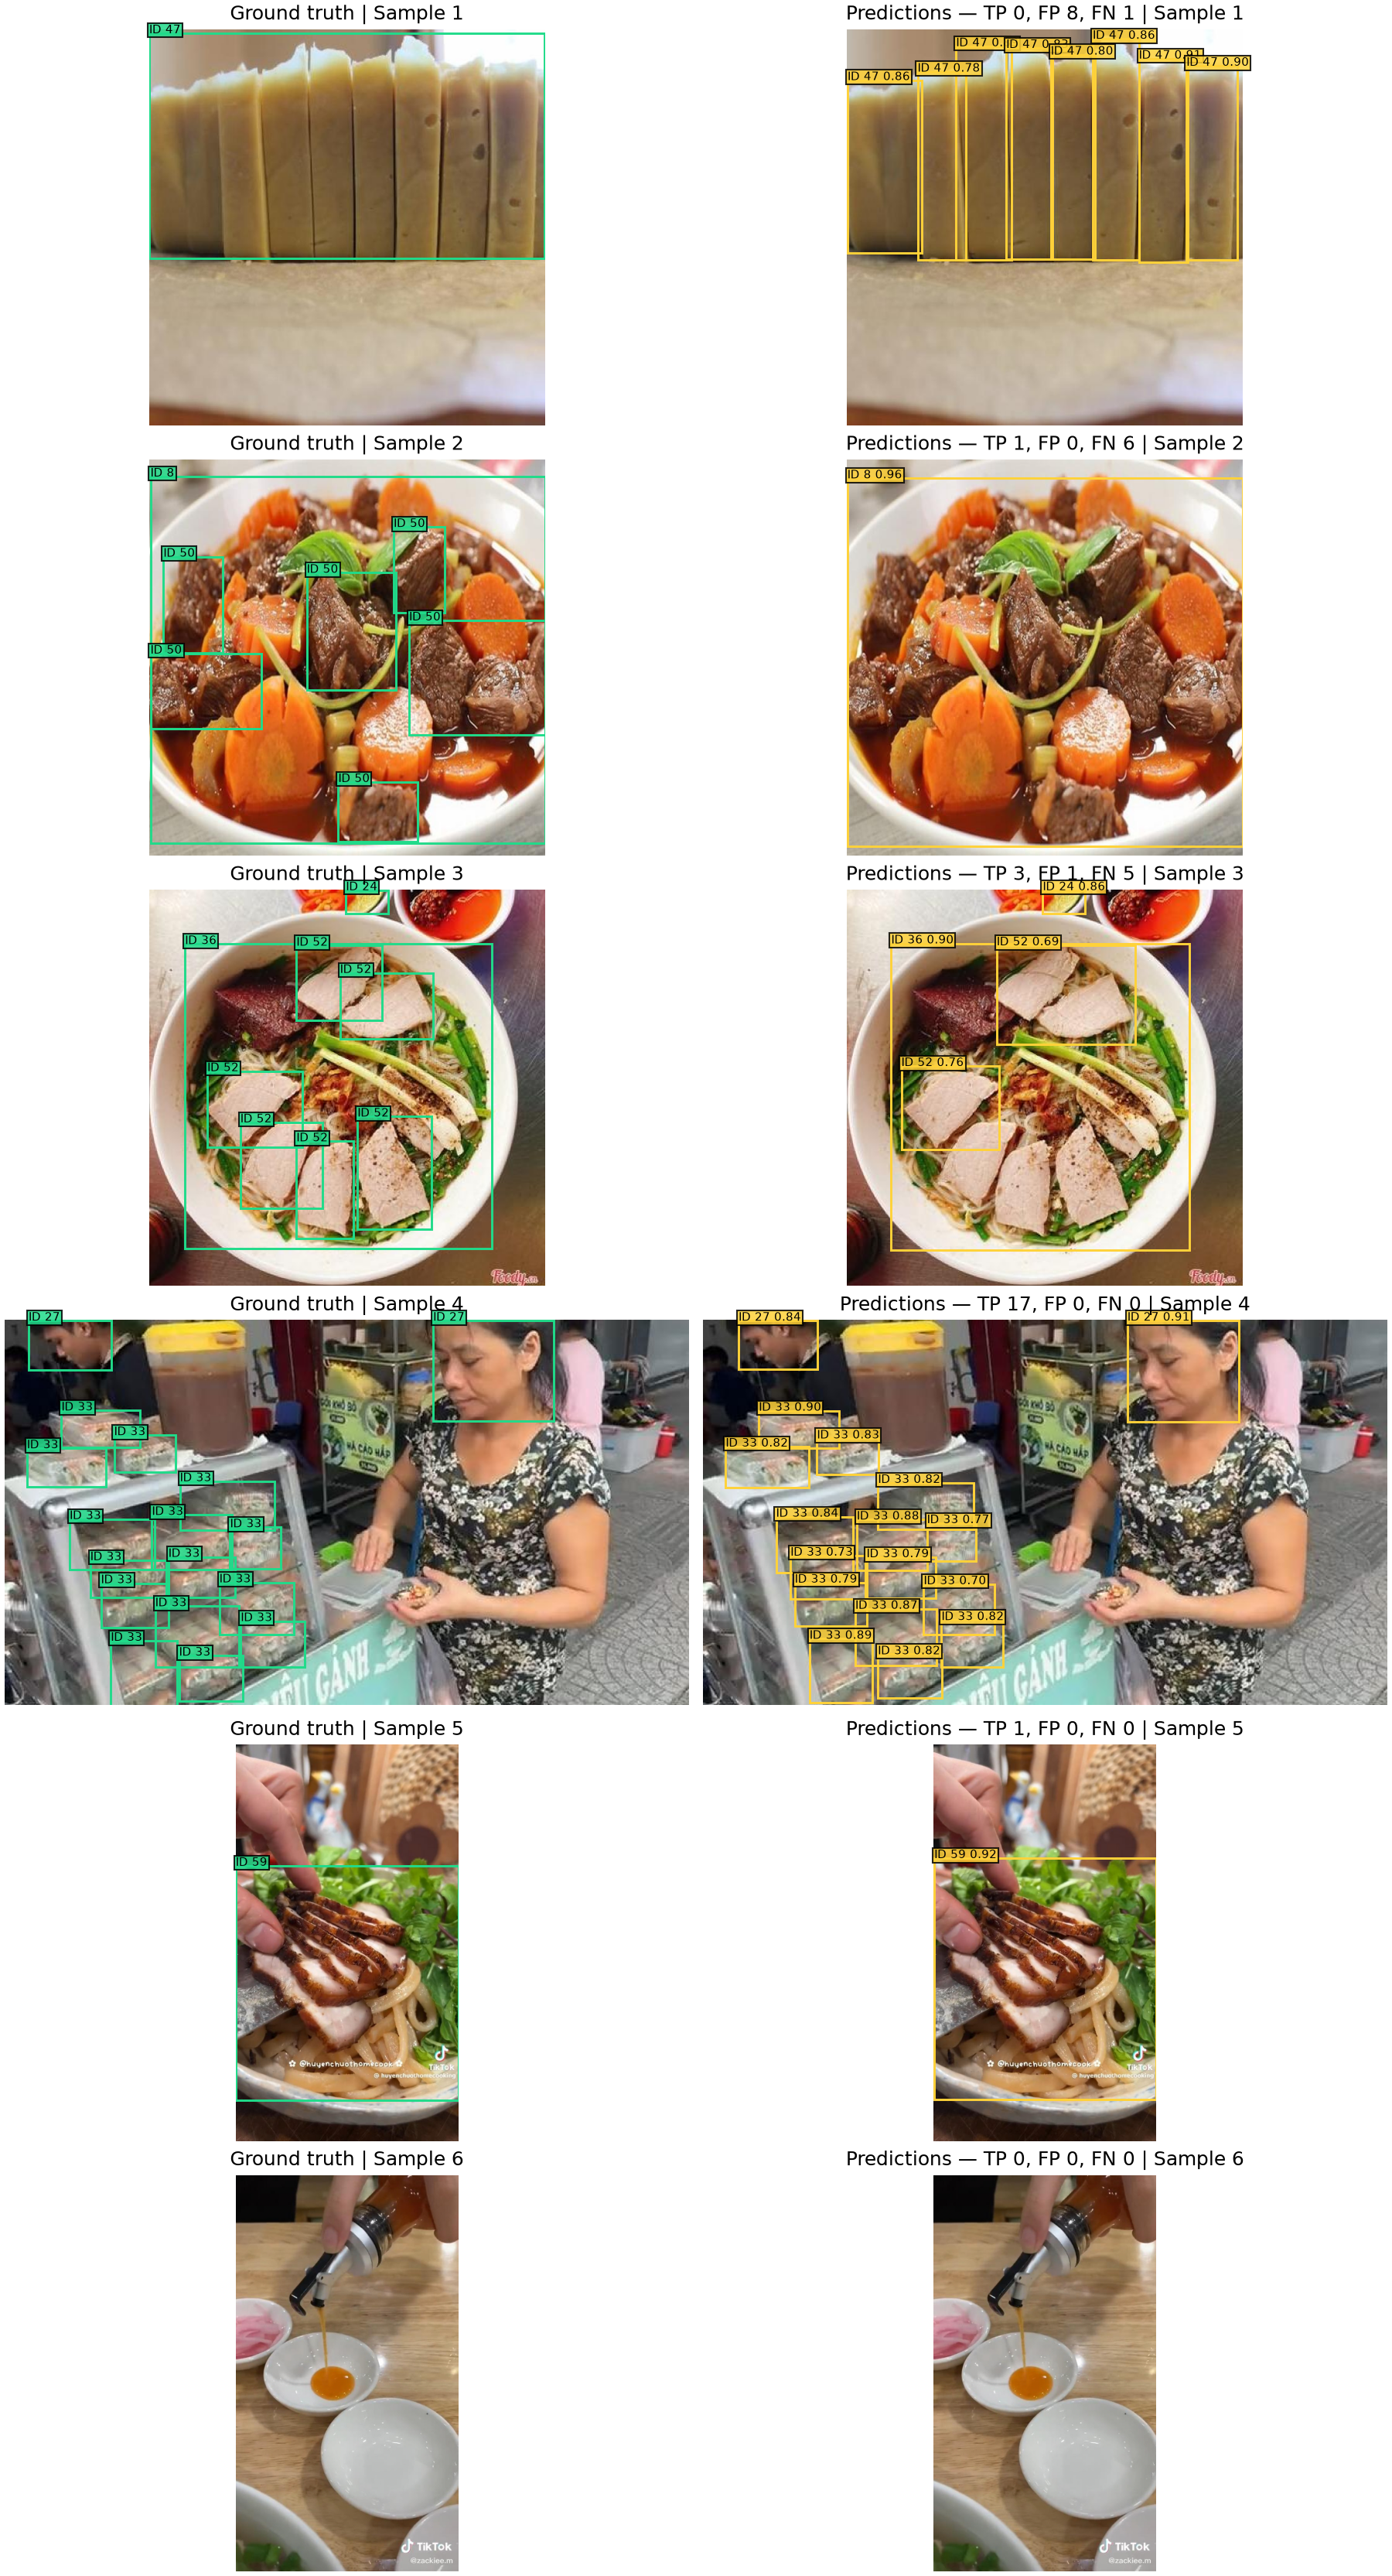
\includegraphics[viewport=0 1065.6 864 1598.4,clip,width=\linewidth,height=0.86\textheight,keepaspectratio]{reports/evaluation/figures/test_error_examples.png}
\par\medskip
{\small\textbf{Hình 5a.} Mẫu 1–2: bên trái là GT, bên phải là dự đoán tại confidence 0,5936.}
\end{landscape}
\begin{landscape}
\centering
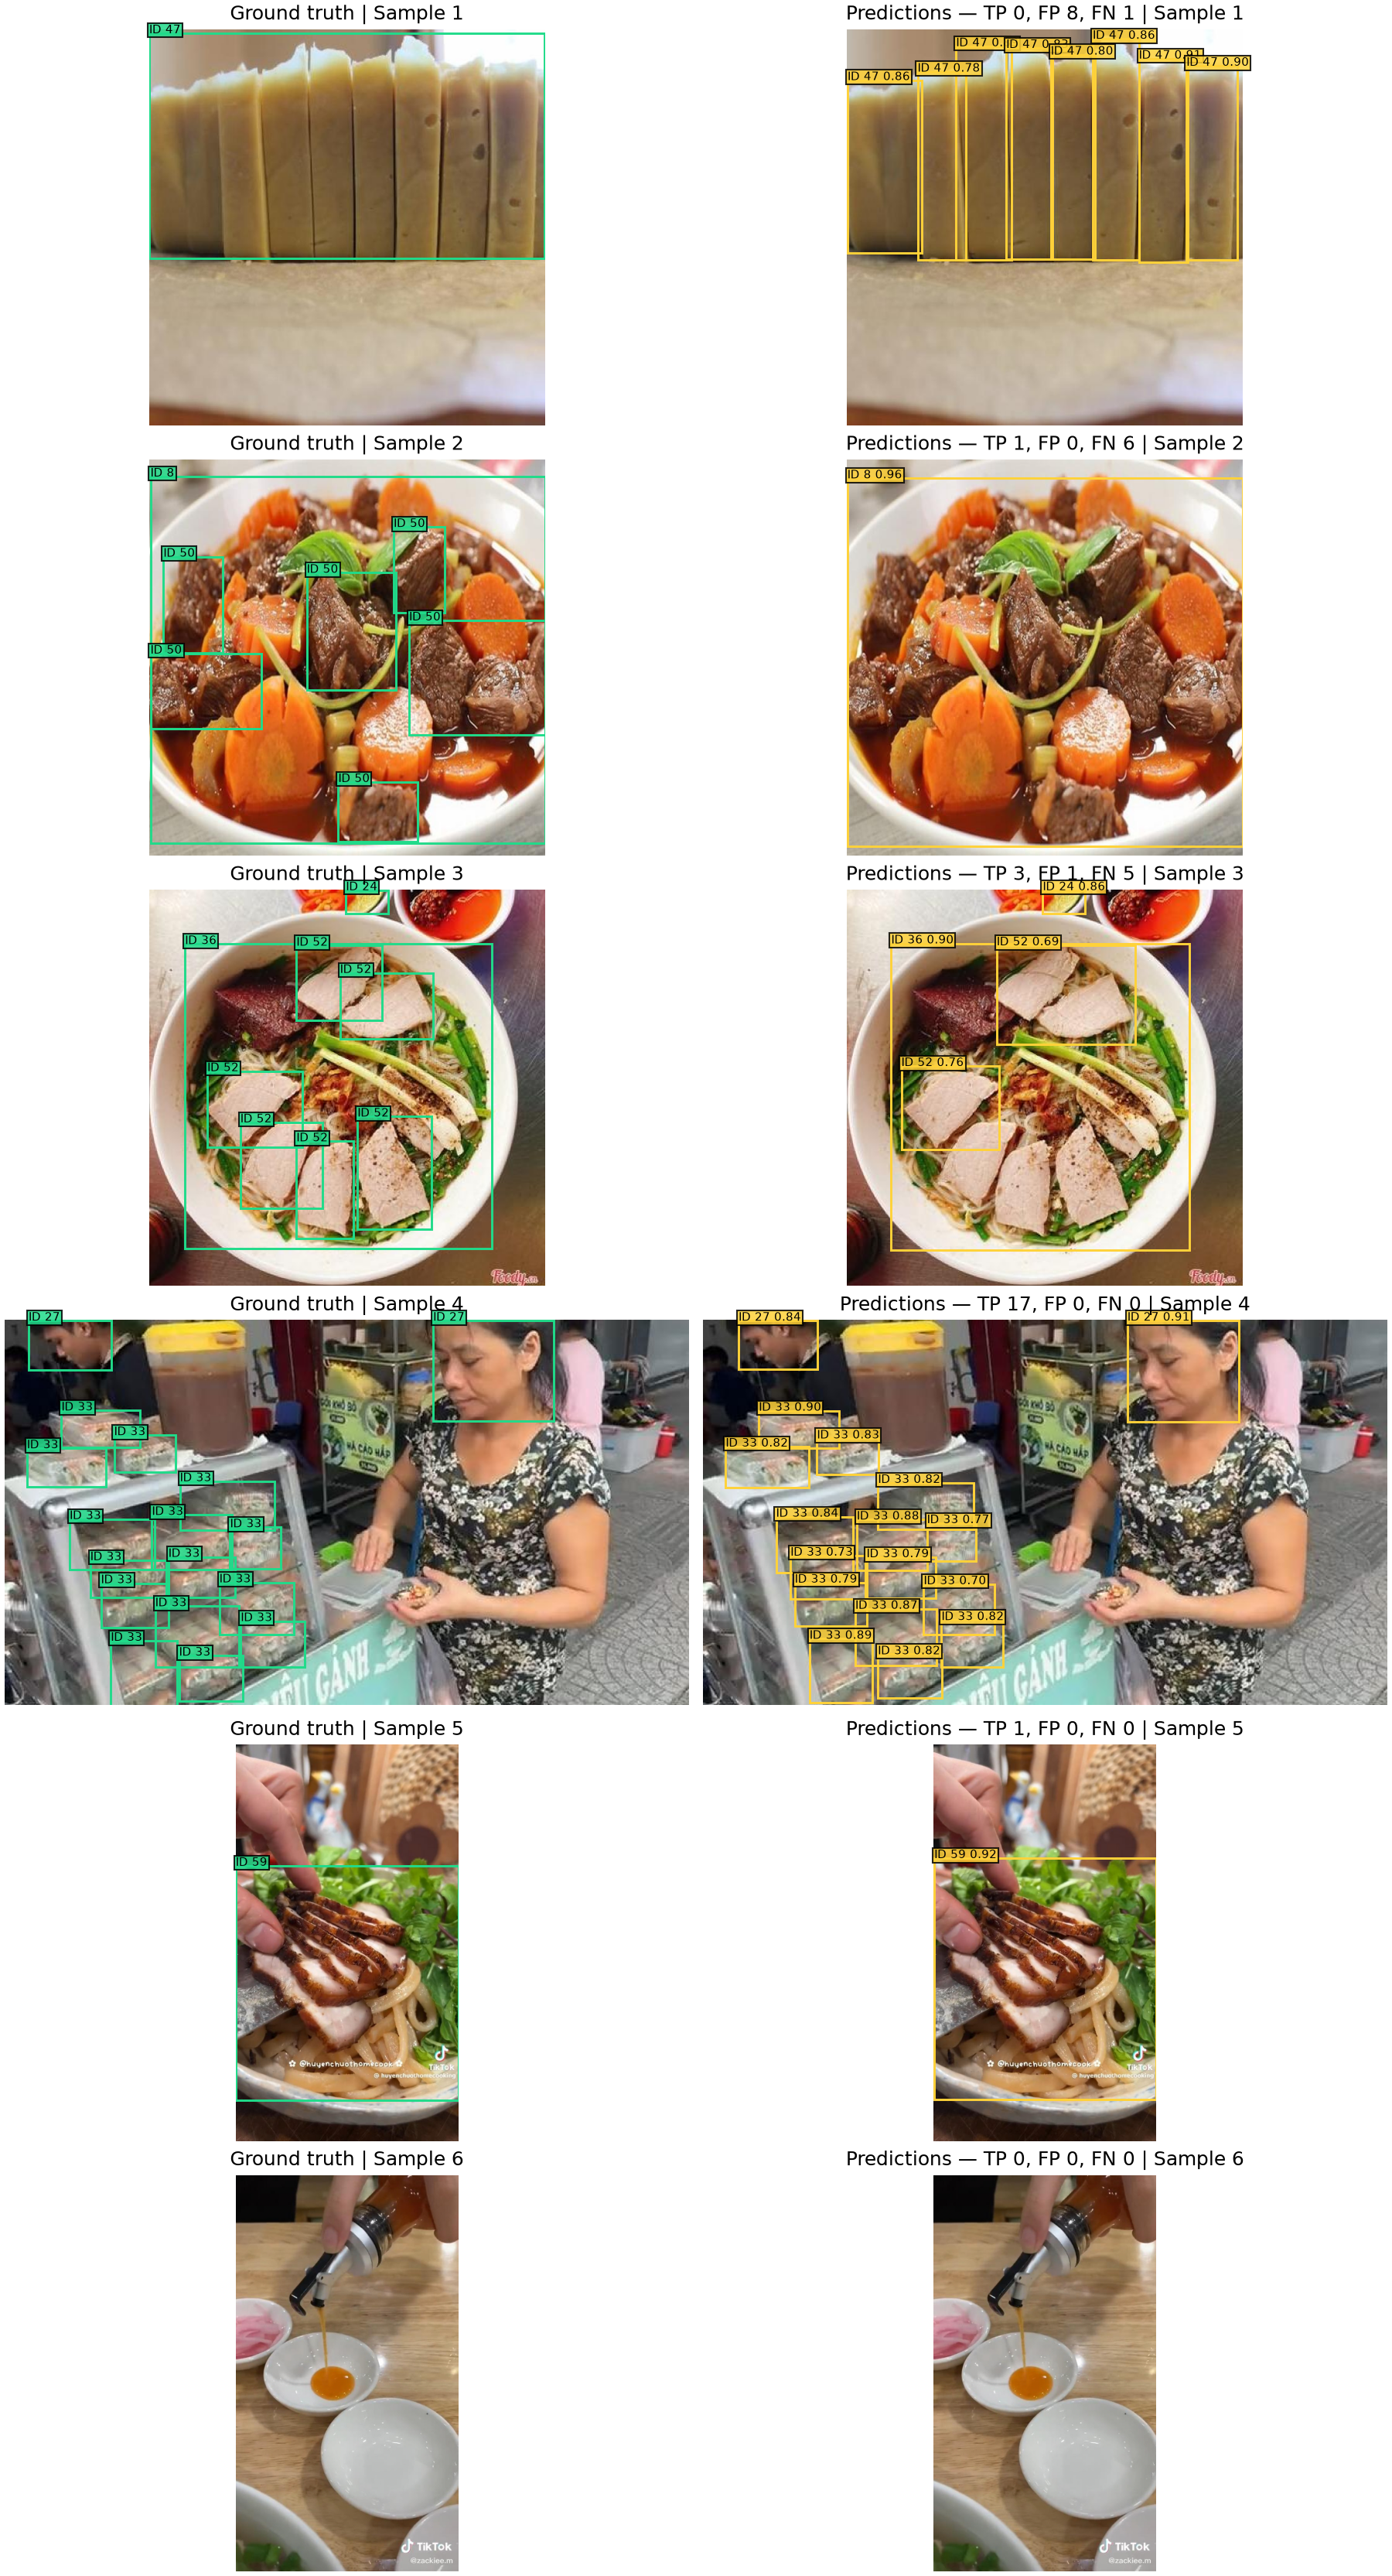
\includegraphics[viewport=0 532.8 864 1065.6,clip,width=\linewidth,height=0.86\textheight,keepaspectratio]{reports/evaluation/figures/test_error_examples.png}
\par\medskip
{\small\textbf{Hình 5b.} Mẫu 3–4: bên trái là GT, bên phải là dự đoán tại confidence 0,5936.}
\end{landscape}
\begin{landscape}
\centering
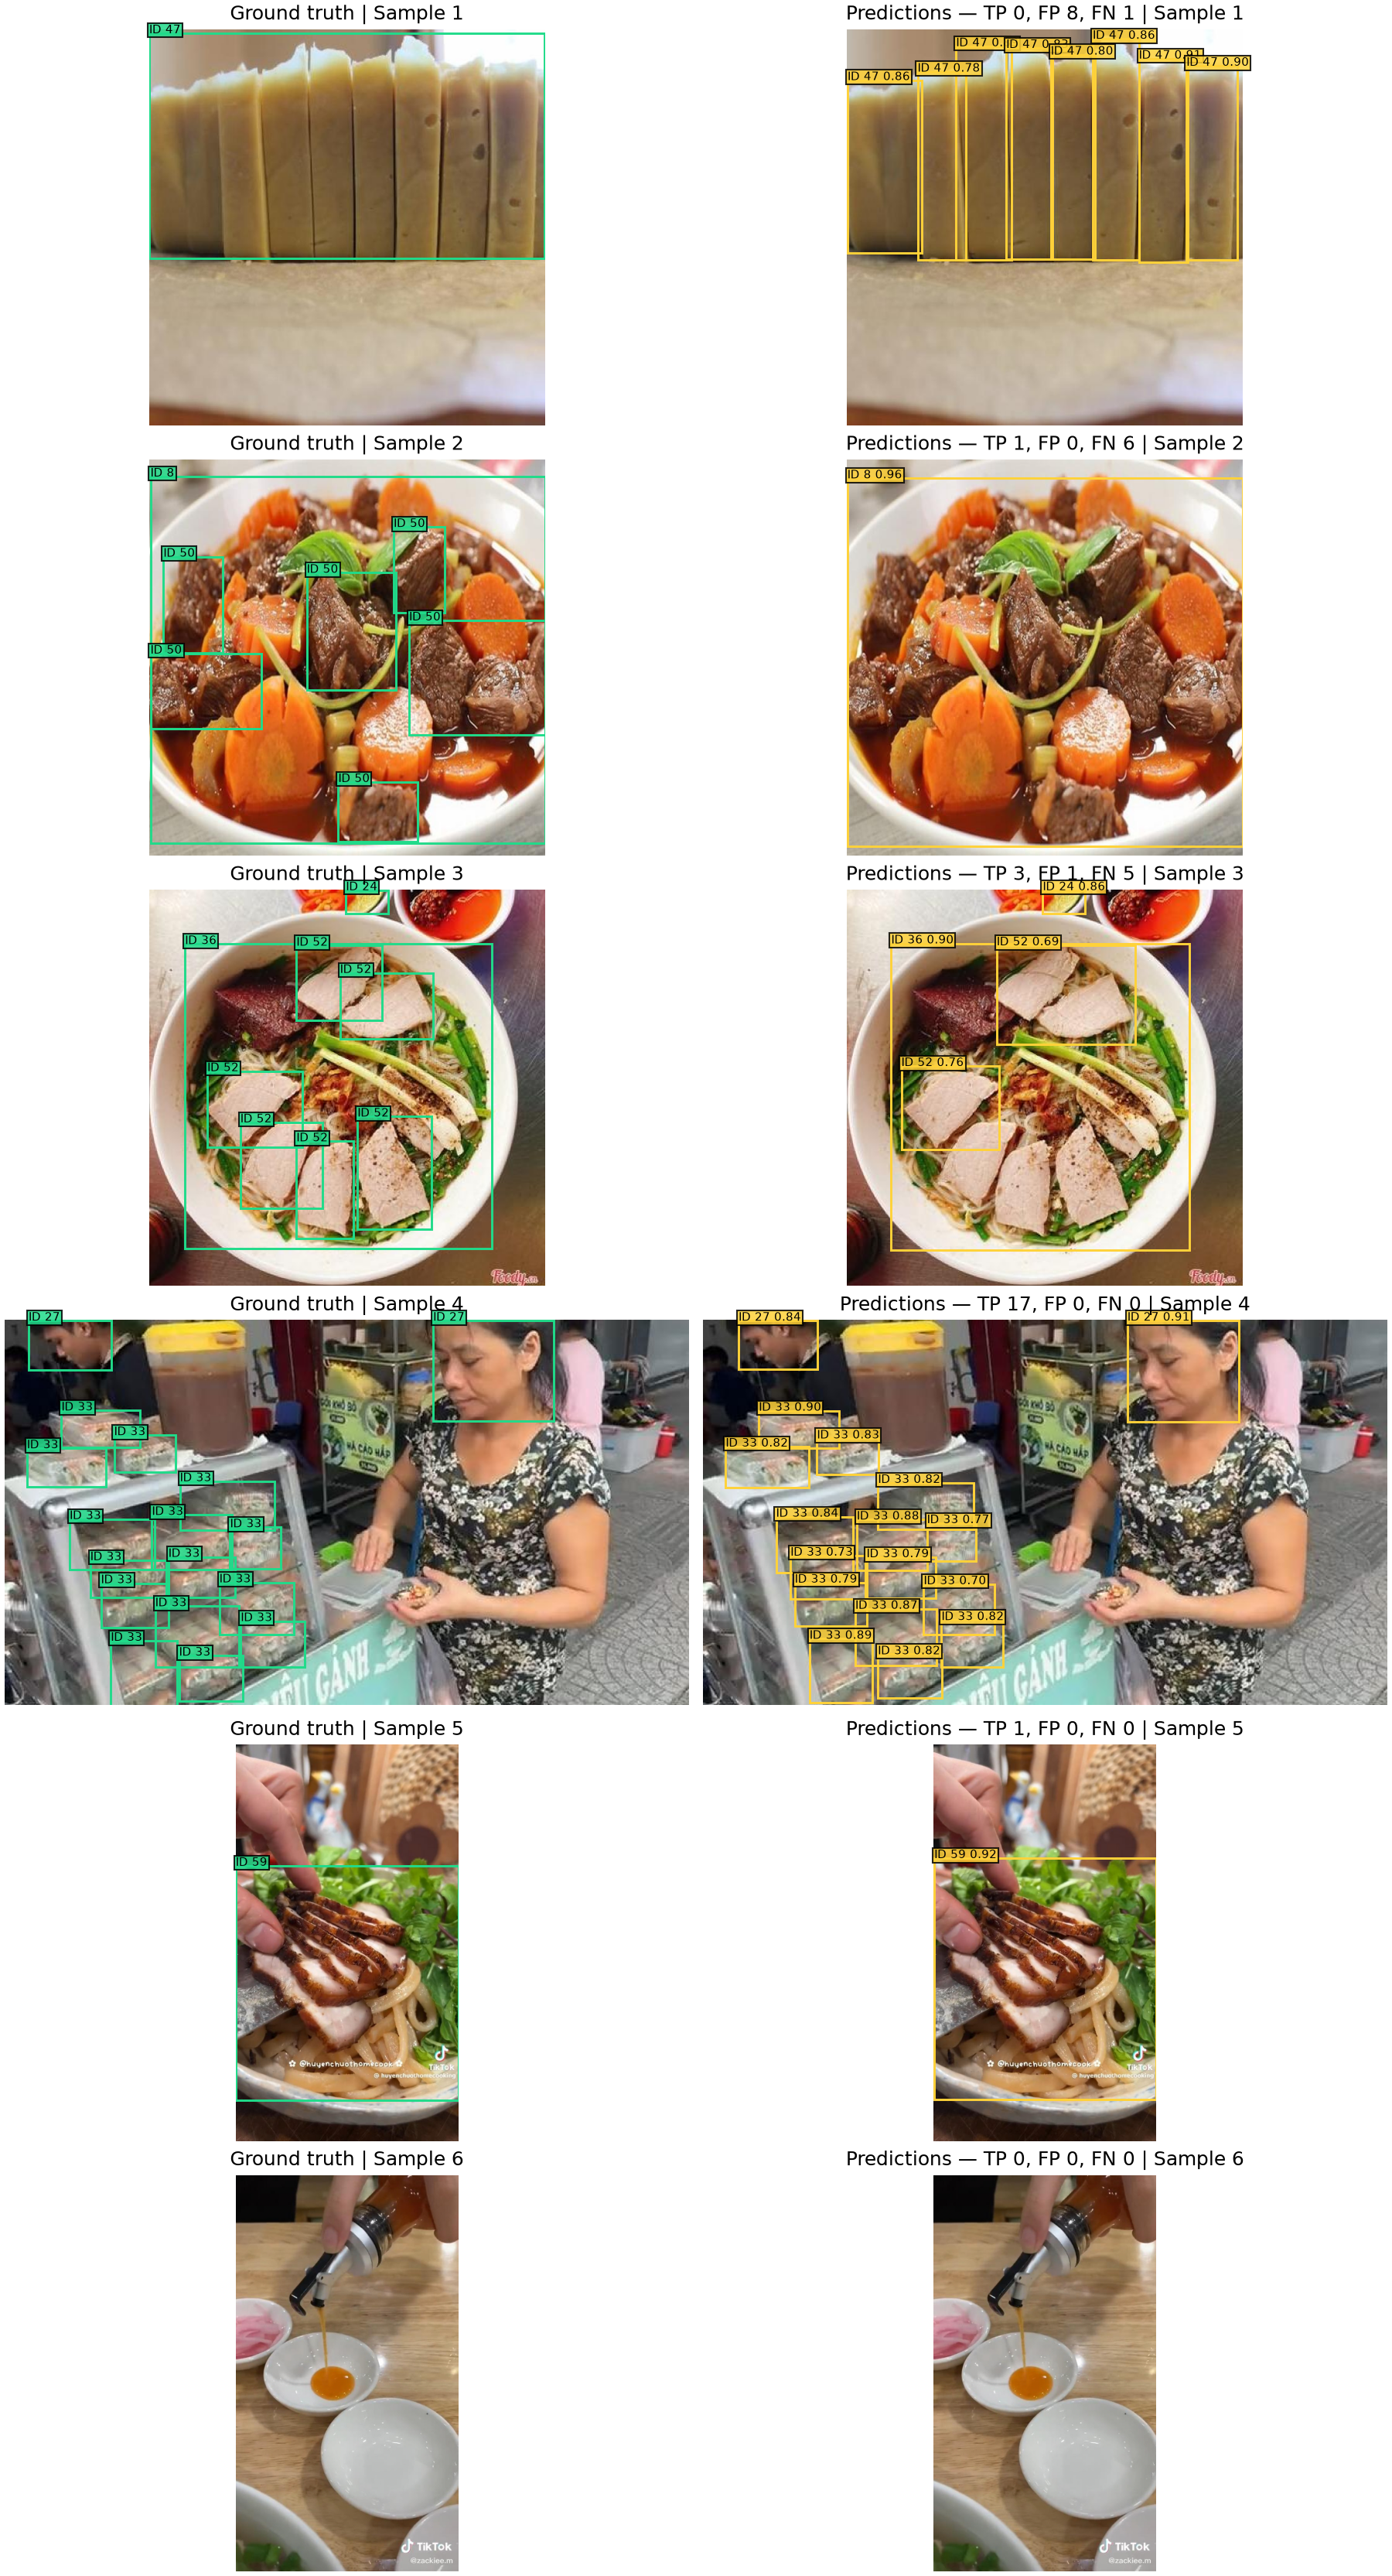
\includegraphics[viewport=0 0.0 864 532.8,clip,width=\linewidth,height=0.86\textheight,keepaspectratio]{reports/evaluation/figures/test_error_examples.png}
\par\medskip
{\small\textbf{Hình 5c.} Mẫu 5–6: bên trái là GT, bên phải là dự đoán tại confidence 0,5936.}
\end{landscape}

\textbf{Hình 5.} Mẫu 1--3 được chọn tự động theo số FP+FN cao nhất. Mẫu
4 là một ảnh nhiều GT được ghép đúng toàn bộ; mẫu 5 là một ảnh đúng khác
trong danh sách; mẫu 6 là ảnh nhãn rỗng không có dự đoán. Đây là ví dụ
phân tích có chủ đích, không phải mẫu ngẫu nhiên đại diện toàn test.

\begingroup\small\setlength{\tabcolsep}{4pt}\renewcommand{\arraystretch}{1.12}

{\def\LTcaptype{none} % do not increment counter
\begin{longtable}[]{@{}
  >{\raggedright\arraybackslash}p{(\linewidth - 10\tabcolsep) * \real{0.0700}}
  >{\raggedright\arraybackslash}p{(\linewidth - 10\tabcolsep) * \real{0.6500}}
  >{\raggedright\arraybackslash}p{(\linewidth - 10\tabcolsep) * \real{0.0700}}
  >{\raggedright\arraybackslash}p{(\linewidth - 10\tabcolsep) * \real{0.0700}}
  >{\raggedright\arraybackslash}p{(\linewidth - 10\tabcolsep) * \real{0.0700}}
  >{\raggedright\arraybackslash}p{(\linewidth - 10\tabcolsep) * \real{0.0700}}@{}}
\toprule\noalign{}
\begin{minipage}[b]{\linewidth}\raggedright
Mẫu
\end{minipage} & \begin{minipage}[b]{\linewidth}\raggedright
File
\end{minipage} & \begin{minipage}[b]{\linewidth}\raggedright
GT
\end{minipage} & \begin{minipage}[b]{\linewidth}\raggedright
TP
\end{minipage} & \begin{minipage}[b]{\linewidth}\raggedright
FP
\end{minipage} & \begin{minipage}[b]{\linewidth}\raggedright
FN
\end{minipage} \\
\midrule\noalign{}
\endhead
\bottomrule\noalign{}
\endlastfoot
1 &
\texttt{1\allowbreak{}0\allowbreak{}a\allowbreak{}5\allowbreak{}1\allowbreak{}0\allowbreak{}e\allowbreak{}4\allowbreak{}8\allowbreak{}4\allowbreak{}c\allowbreak{}0\allowbreak{}f\allowbreak{}1\allowbreak{}e\allowbreak{}6\allowbreak{}\_\allowbreak{}j\allowbreak{}p\allowbreak{}g\allowbreak{}.\allowbreak{}r\allowbreak{}f\allowbreak{}.\allowbreak{}6\allowbreak{}6\allowbreak{}d\allowbreak{}7\allowbreak{}3\allowbreak{}3\allowbreak{}7\allowbreak{}8\allowbreak{}9\allowbreak{}2\allowbreak{}8\allowbreak{}8\allowbreak{}3\allowbreak{}6\allowbreak{}1\allowbreak{}5\allowbreak{}2\allowbreak{}0\allowbreak{}f\allowbreak{}1\allowbreak{}4\allowbreak{}c\allowbreak{}f\allowbreak{}f\allowbreak{}1\allowbreak{}8\allowbreak{}5\allowbreak{}b\allowbreak{}6\allowbreak{}d\allowbreak{}2\allowbreak{}b\allowbreak{}.\allowbreak{}j\allowbreak{}p\allowbreak{}g\allowbreak{}}
& 1 & 0 & 8 & 1 \\
2 &
\texttt{4\allowbreak{}4\allowbreak{}\_\allowbreak{}j\allowbreak{}p\allowbreak{}g\allowbreak{}.\allowbreak{}r\allowbreak{}f\allowbreak{}.\allowbreak{}b\allowbreak{}a\allowbreak{}3\allowbreak{}5\allowbreak{}5\allowbreak{}1\allowbreak{}9\allowbreak{}3\allowbreak{}b\allowbreak{}9\allowbreak{}a\allowbreak{}3\allowbreak{}3\allowbreak{}6\allowbreak{}8\allowbreak{}f\allowbreak{}e\allowbreak{}4\allowbreak{}1\allowbreak{}2\allowbreak{}3\allowbreak{}3\allowbreak{}2\allowbreak{}1\allowbreak{}6\allowbreak{}2\allowbreak{}6\allowbreak{}1\allowbreak{}0\allowbreak{}3\allowbreak{}7\allowbreak{}2\allowbreak{}.\allowbreak{}j\allowbreak{}p\allowbreak{}g\allowbreak{}}
& 7 & 1 & 0 & 6 \\
3 &
\texttt{3\allowbreak{}3\allowbreak{}\_\allowbreak{}j\allowbreak{}p\allowbreak{}g\allowbreak{}.\allowbreak{}r\allowbreak{}f\allowbreak{}.\allowbreak{}5\allowbreak{}7\allowbreak{}1\allowbreak{}2\allowbreak{}2\allowbreak{}5\allowbreak{}5\allowbreak{}0\allowbreak{}6\allowbreak{}0\allowbreak{}3\allowbreak{}c\allowbreak{}1\allowbreak{}d\allowbreak{}6\allowbreak{}c\allowbreak{}7\allowbreak{}f\allowbreak{}d\allowbreak{}d\allowbreak{}d\allowbreak{}4\allowbreak{}7\allowbreak{}b\allowbreak{}1\allowbreak{}1\allowbreak{}1\allowbreak{}3\allowbreak{}3\allowbreak{}3\allowbreak{}8\allowbreak{}b\allowbreak{}.\allowbreak{}j\allowbreak{}p\allowbreak{}g\allowbreak{}}
& 8 & 3 & 1 & 5 \\
4 &
\texttt{y\allowbreak{}t\allowbreak{}-\allowbreak{}Q\allowbreak{}z\allowbreak{}b\allowbreak{}N\allowbreak{}s\allowbreak{}S\allowbreak{}r\allowbreak{}M\allowbreak{}o\allowbreak{}K\allowbreak{}E\allowbreak{}-\allowbreak{}0\allowbreak{}0\allowbreak{}3\allowbreak{}8\allowbreak{}\_\allowbreak{}j\allowbreak{}p\allowbreak{}g\allowbreak{}.\allowbreak{}r\allowbreak{}f\allowbreak{}.\allowbreak{}9\allowbreak{}a\allowbreak{}1\allowbreak{}a\allowbreak{}d\allowbreak{}8\allowbreak{}4\allowbreak{}f\allowbreak{}4\allowbreak{}1\allowbreak{}d\allowbreak{}c\allowbreak{}7\allowbreak{}a\allowbreak{}6\allowbreak{}3\allowbreak{}0\allowbreak{}e\allowbreak{}b\allowbreak{}b\allowbreak{}6\allowbreak{}1\allowbreak{}3\allowbreak{}a\allowbreak{}a\allowbreak{}7\allowbreak{}d\allowbreak{}2\allowbreak{}5\allowbreak{}f\allowbreak{}b\allowbreak{}7\allowbreak{}.\allowbreak{}j\allowbreak{}p\allowbreak{}g\allowbreak{}}
& 17 & 17 & 0 & 0 \\
5 &
\texttt{D\allowbreak{}o\allowbreak{}w\allowbreak{}n\allowbreak{}l\allowbreak{}o\allowbreak{}a\allowbreak{}d\allowbreak{}-\allowbreak{}8\allowbreak{}-\allowbreak{}\_\allowbreak{}m\allowbreak{}p\allowbreak{}4\allowbreak{}-\allowbreak{}0\allowbreak{}0\allowbreak{}4\allowbreak{}0\allowbreak{}\_\allowbreak{}j\allowbreak{}p\allowbreak{}g\allowbreak{}.\allowbreak{}r\allowbreak{}f\allowbreak{}.\allowbreak{}4\allowbreak{}5\allowbreak{}9\allowbreak{}b\allowbreak{}f\allowbreak{}e\allowbreak{}7\allowbreak{}4\allowbreak{}9\allowbreak{}e\allowbreak{}a\allowbreak{}3\allowbreak{}4\allowbreak{}7\allowbreak{}a\allowbreak{}8\allowbreak{}1\allowbreak{}f\allowbreak{}4\allowbreak{}a\allowbreak{}5\allowbreak{}8\allowbreak{}c\allowbreak{}1\allowbreak{}3\allowbreak{}4\allowbreak{}d\allowbreak{}9\allowbreak{}8\allowbreak{}b\allowbreak{}c\allowbreak{}e\allowbreak{}.\allowbreak{}j\allowbreak{}p\allowbreak{}g\allowbreak{}}
& 1 & 1 & 0 & 0 \\
6 &
\texttt{D\allowbreak{}o\allowbreak{}w\allowbreak{}n\allowbreak{}l\allowbreak{}o\allowbreak{}a\allowbreak{}d\allowbreak{}-\allowbreak{}1\allowbreak{}-\allowbreak{}\_\allowbreak{}m\allowbreak{}p\allowbreak{}4\allowbreak{}-\allowbreak{}0\allowbreak{}0\allowbreak{}3\allowbreak{}6\allowbreak{}\_\allowbreak{}j\allowbreak{}p\allowbreak{}g\allowbreak{}.\allowbreak{}r\allowbreak{}f\allowbreak{}.\allowbreak{}9\allowbreak{}2\allowbreak{}6\allowbreak{}a\allowbreak{}3\allowbreak{}8\allowbreak{}2\allowbreak{}4\allowbreak{}b\allowbreak{}6\allowbreak{}d\allowbreak{}0\allowbreak{}7\allowbreak{}2\allowbreak{}a\allowbreak{}2\allowbreak{}e\allowbreak{}5\allowbreak{}e\allowbreak{}3\allowbreak{}7\allowbreak{}e\allowbreak{}2\allowbreak{}d\allowbreak{}c\allowbreak{}e\allowbreak{}d\allowbreak{}a\allowbreak{}1\allowbreak{}d\allowbreak{}2\allowbreak{}3\allowbreak{}.\allowbreak{}j\allowbreak{}p\allowbreak{}g\allowbreak{}}
& 0 & 0 & 0 & 0 \\
\end{longtable}
}

\endgroup

Mẫu 1 có GT
\texttt{c\allowbreak{}l\allowbreak{}a\allowbreak{}s\allowbreak{}s\allowbreak{}\_\allowbreak{}4\allowbreak{}7\allowbreak{}}
bao cả khối, còn dự đoán tách thành tám phần; cả tám không đạt điều kiện
IoU với hộp lớn. Cần thống nhất ``một đối tượng'' là cả khối hay từng
miếng. Mẫu 2 giữ được hộp món lớn
\texttt{c\allowbreak{}l\allowbreak{}a\allowbreak{}s\allowbreak{}s\allowbreak{}\_\allowbreak{}8\allowbreak{}}
nhưng bỏ các hộp thành phần
\texttt{c\allowbreak{}l\allowbreak{}a\allowbreak{}s\allowbreak{}s\allowbreak{}\_\allowbreak{}5\allowbreak{}0\allowbreak{}}.
Mẫu 3 cho thấy các hộp thành phần chồng lấp và một số hộp nhỏ bị bỏ sót.

Mẫu 4 đặc biệt đáng chú ý: GT
\texttt{c\allowbreak{}l\allowbreak{}a\allowbreak{}s\allowbreak{}s\allowbreak{}\_\allowbreak{}2\allowbreak{}7\allowbreak{}}
bao quanh khuôn mặt/người, cùng nhiều GT
\texttt{c\allowbreak{}l\allowbreak{}a\allowbreak{}s\allowbreak{}s\allowbreak{}\_\allowbreak{}3\allowbreak{}3\allowbreak{}}.
Quan sát này phù hợp với lớp người trong nguồn tham chiếu, nên
\textbf{68 ID không được mô tả là 68 món ăn}. Việc nhiều hộp cùng một
ảnh được ghép đúng cũng không thay thế đánh giá theo lớp hoặc tập ngoài
miền.

\subsection{8.3. Ma trận nhầm lẫn tại ngưỡng vận
hành}\label{ma-trux1eadn-nhux1ea7m-lux1eabn-tux1ea1i-ngux1b0ux1ee1ng-vux1eadn-huxe0nh}

\begin{center}
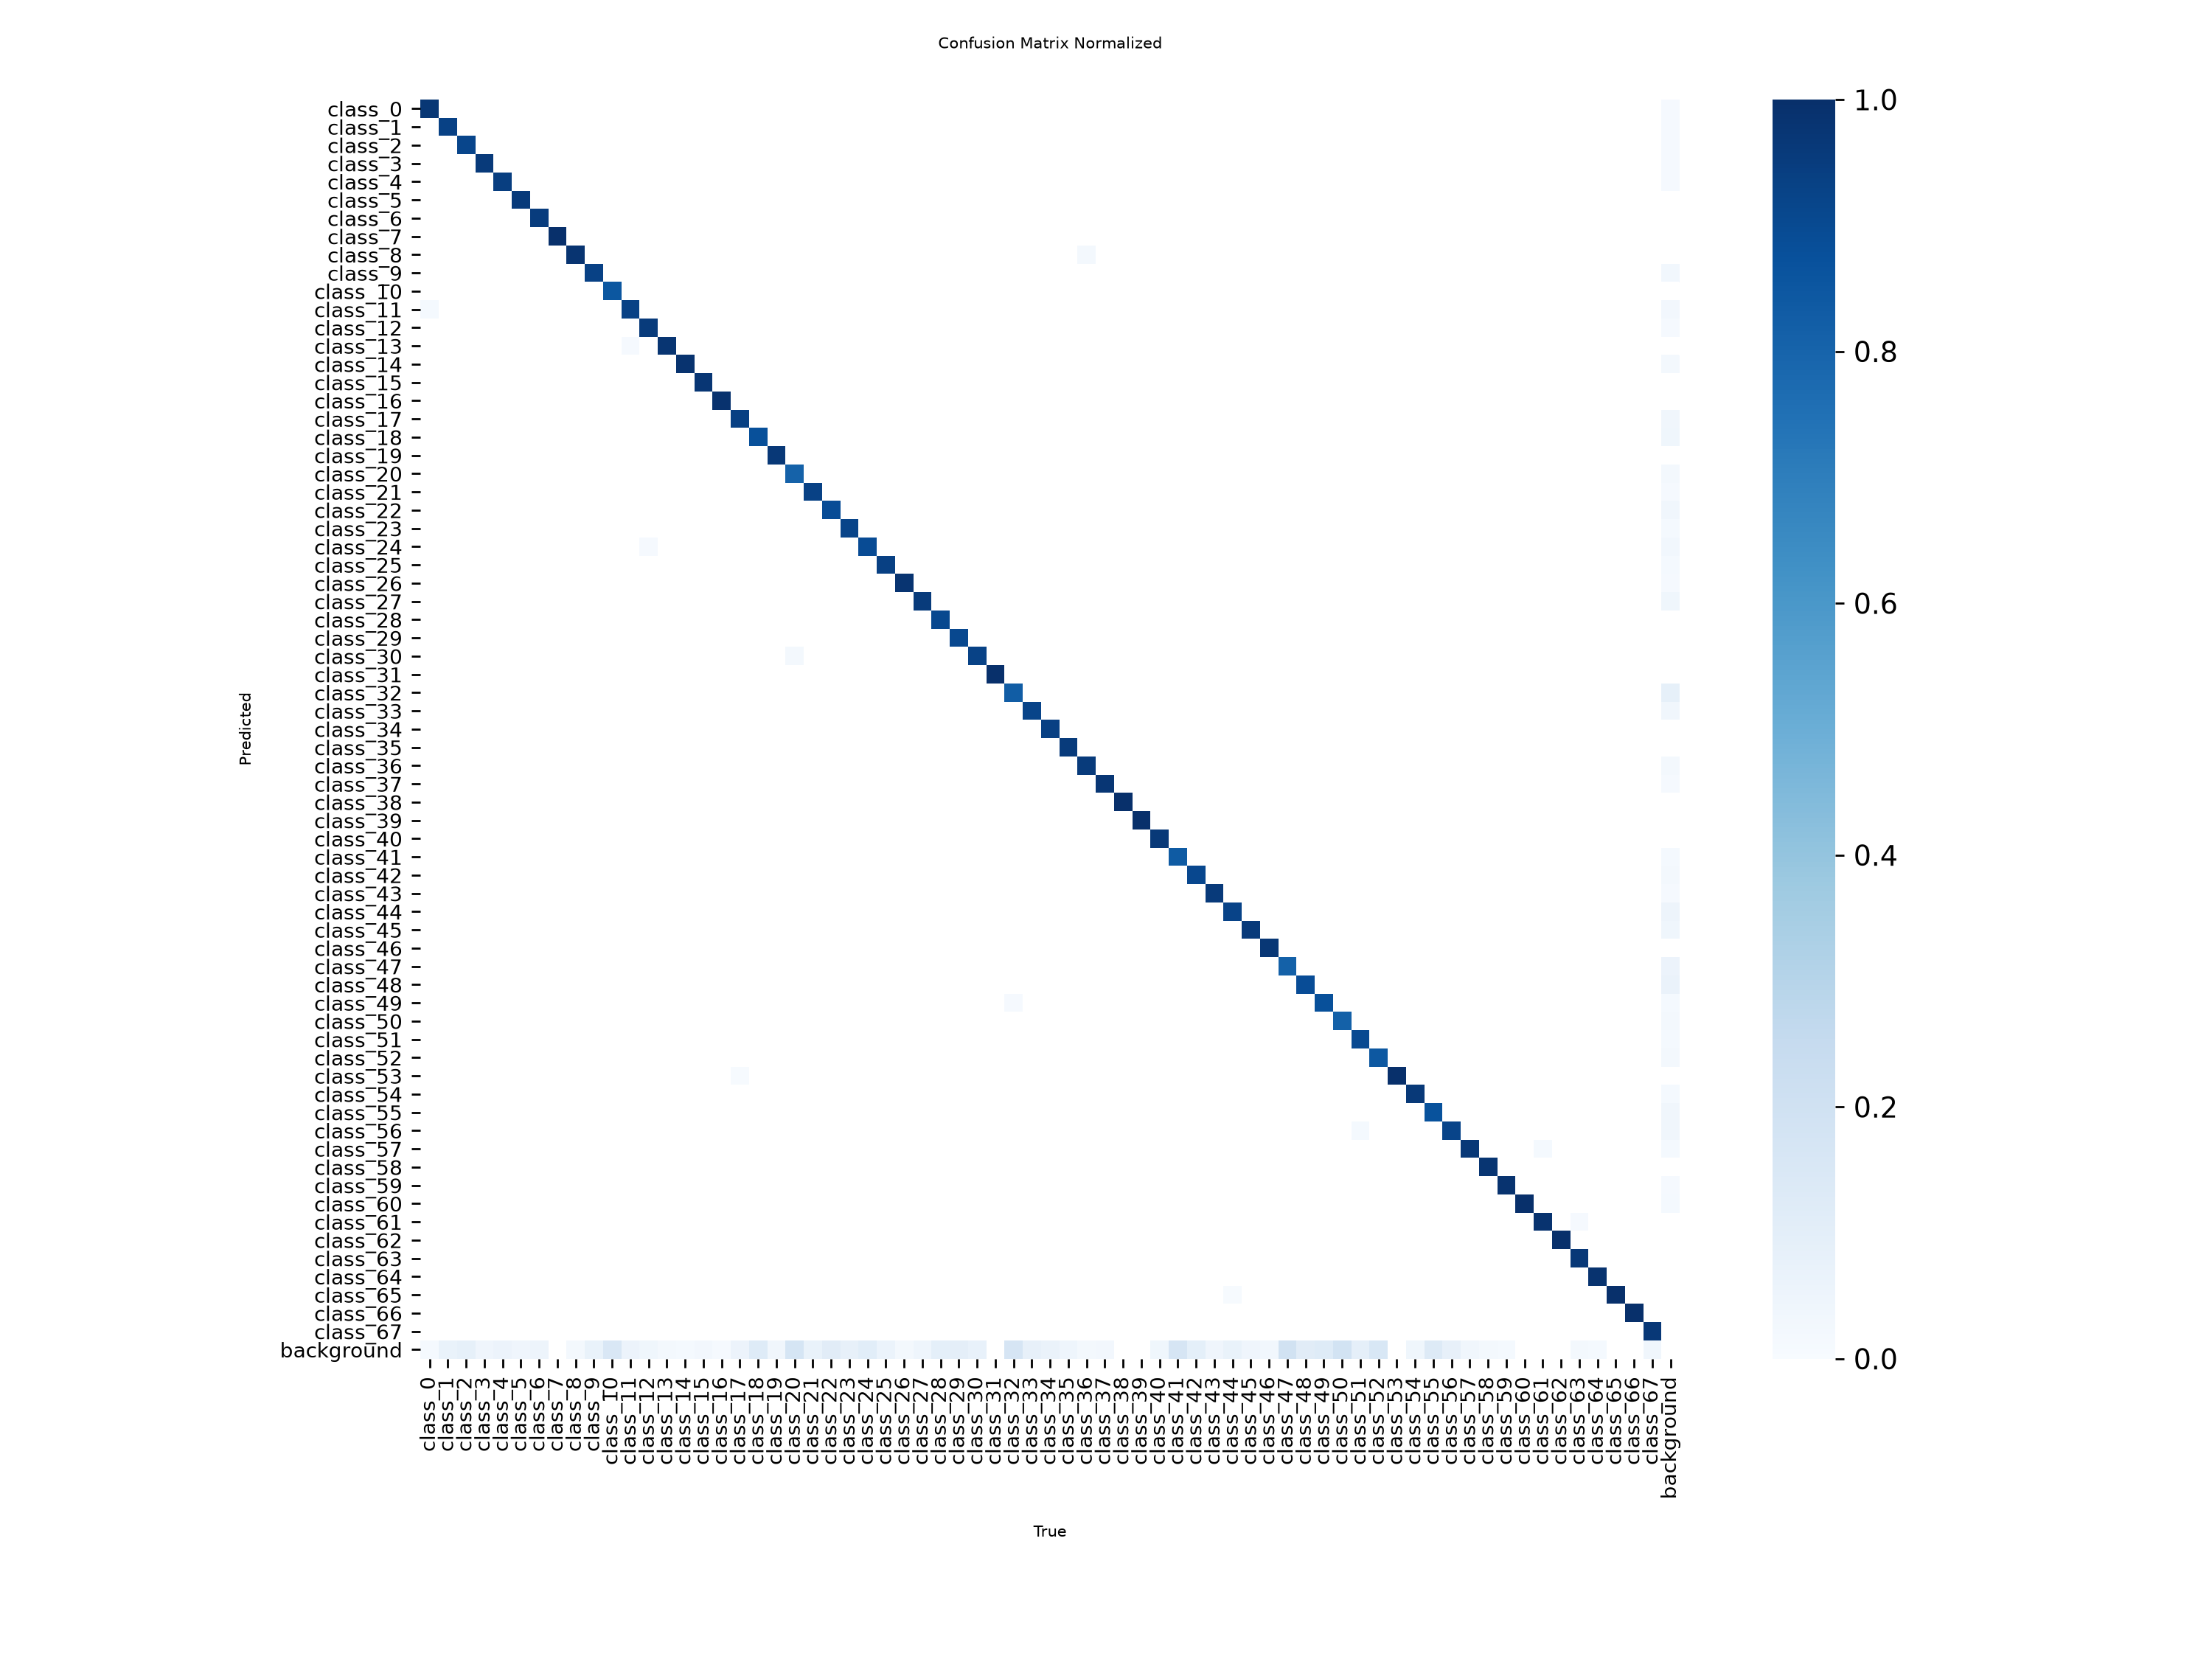
\includegraphics[width=\linewidth,height=0.76\textheight,keepaspectratio]{reports/evaluation/figures/test_operating_confusion_matrix.png}
\end{center}

\textbf{Hình 6.} Hàng dự đoán, cột GT. Ô nền bao gồm FP/FN theo quy tắc
matrix. Bản đủ số đếm tại
\href{reports/evaluation/test_operating_confusion_matrix.csv}{test\_operating\_confusion\_matrix.csv}.

Các cặp nhầm lớp hình học đứng đầu chỉ xuất hiện một lần mỗi cặp, ví dụ
GT 36 → dự đoán 8, GT 20 → dự đoán 30, GT 32 → dự đoán 49. Vì hỗ trợ ít,
chưa có cơ sở kết luận một cặp món cụ thể bị nhầm thường xuyên. Rà soát
định vị, bỏ sót và annotation có ưu tiên cao hơn việc suy diễn tên món
từ ID.

\subsection{8.4. Kiểm thử và bằng
chứng}\label{kiux1ec3m-thux1eed-vuxe0-bux1eb1ng-chux1ee9ng}

\begingroup\small\setlength{\tabcolsep}{4pt}\renewcommand{\arraystretch}{1.12}

{\def\LTcaptype{none} % do not increment counter
\begin{longtable}[]{@{}
  >{\raggedright\arraybackslash}p{(\linewidth - 4\tabcolsep) * \real{0.2300}}
  >{\raggedright\arraybackslash}p{(\linewidth - 4\tabcolsep) * \real{0.3400}}
  >{\raggedright\arraybackslash}p{(\linewidth - 4\tabcolsep) * \real{0.4300}}@{}}
\toprule\noalign{}
\begin{minipage}[b]{\linewidth}\raggedright
Mã
\end{minipage} & \begin{minipage}[b]{\linewidth}\raggedright
Nội dung
\end{minipage} & \begin{minipage}[b]{\linewidth}\raggedright
Kết quả và bằng chứng
\end{minipage} \\
\midrule\noalign{}
\endhead
\bottomrule\noalign{}
\endlastfoot
T01 & Ghép ảnh--nhãn và kiểm tra định dạng & Đạt về cấu trúc; audit toàn
bộ nhãn, 0 lỗi \\
T02 & Đủ các ID được cấu hình & Đạt; 68/68 ID ở cả ba tập \\
T03 & Trùng file byte giữa các tập & Không phát hiện; SHA-256 và lọc
kích thước \\
T04 & Đọc và đánh giá toàn validation/test & Đạt; 6.602 và 3.284 ảnh đã
xử lý \\
T05 & Checkpoint đúng kiến trúc và có thể suy luận & Đạt; cấu hình
YOLO11s, 68 lớp và benchmark \\
T06 & TP/FP/FN tại ngưỡng khóa & Đạt đối chiếu; đếm từ evaluator và ghép
lại JSON trùng nhau \\
T07 & Bộ nạp dữ liệu và resume batch & Đạt 3 kiểm thử; kiểm thử trong
thư mục
\texttt{t\allowbreak{}e\allowbreak{}s\allowbreak{}t\allowbreak{}s\allowbreak{}} \\
T08 & Tên món hiển thị đúng & Chưa kiểm chứng toàn bộ; thiếu mapping cục
bộ gốc \\
T09 & Giao diện Streamlit, upload, ảnh lỗi & Chưa thực hiện; chưa có app
trong repo \\
T10 & Dữ liệu ngoài miền, video/webcam và nhiều người dùng & Chưa thực
hiện \\
\end{longtable}
}

\endgroup

``Đạt'' ở T01--T07 có phạm vi cụ thể của phép kiểm tra, không đồng nghĩa
hệ thống sẵn sàng triển khai sản phẩm. Bằng chứng máy đọc được nằm trong
\texttt{r\allowbreak{}e\allowbreak{}p\allowbreak{}o\allowbreak{}r\allowbreak{}t\allowbreak{}s\allowbreak{}/\allowbreak{}e\allowbreak{}v\allowbreak{}a\allowbreak{}l\allowbreak{}u\allowbreak{}a\allowbreak{}t\allowbreak{}i\allowbreak{}o\allowbreak{}n\allowbreak{}},
log chạy lưu ở thư mục
\texttt{r\allowbreak{}e\allowbreak{}p\allowbreak{}o\allowbreak{}r\allowbreak{}t\allowbreak{}s\allowbreak{}}.

\section{9. THIẾT KẾ ỨNG DỤNG VÀ HƯỚNG PHÁT
TRIỂN}\label{thiux1ebft-kux1ebf-ux1ee9ng-dux1ee5ng-vuxe0-hux1b0ux1edbng-phuxe1t-triux1ec3n}

\subsection{9.1. Thiết kế giao diện đề
xuất}\label{thiux1ebft-kux1ebf-giao-diux1ec7n-ux111ux1ec1-xuux1ea5t}

Một ứng dụng Streamlit có thể nhận ảnh tải lên, giải mã ảnh, gọi model
đã được cache và hiển thị hộp cùng bảng kết quả.
\texttt{s\allowbreak{}t\allowbreak{}.\allowbreak{}f\allowbreak{}i\allowbreak{}l\allowbreak{}e\allowbreak{}\_\allowbreak{}u\allowbreak{}p\allowbreak{}l\allowbreak{}o\allowbreak{}a\allowbreak{}d\allowbreak{}e\allowbreak{}r\allowbreak{}}
là thành phần phù hợp để nhận ảnh. Phần này là \textbf{thiết kế đề
xuất}, không có ảnh giao diện hoặc trạng thái kiểm thử đạt vì repo hiện
chưa triển khai app.
\href{https://docs.streamlit.io/develop/api-reference/widgets/st.file_uploader}{15}

\begin{center}
\begin{tikzpicture}[every node/.style={draw=blue!55!black,fill=blue!4,rounded corners=2pt,text width=4.1cm,minimum height=1.55cm,align=center,font=\small},>=stealth]
\node (n1) at (0.00,0.00) {Người dùng tải ảnh};
\node (n2) at (4.90,0.00) {Kiểm tra định dạng và kích thước};
\node (n3) at (9.80,0.00) {YOLO11s và ngưỡng đã chọn};
\node (n4) at (9.80,-2.20) {Ánh xạ ID đã xác minh};
\node (n5) at (4.90,-2.20) {Ảnh có hộp và bảng kết quả};
\draw[->,thick,blue!55!black] (n1) -- (n2);
\draw[->,thick,blue!55!black] (n2) -- (n3);
\draw[->,thick,blue!55!black] (n3) -- (n4);
\draw[->,thick,blue!55!black] (n4) -- (n5);
\end{tikzpicture}
\end{center}

\begingroup\small\setlength{\tabcolsep}{4pt}\renewcommand{\arraystretch}{1.12}

{\def\LTcaptype{none} % do not increment counter
\begin{longtable}[]{@{}
  >{\raggedright\arraybackslash}p{(\linewidth - 2\tabcolsep) * \real{0.3200}}
  >{\raggedright\arraybackslash}p{(\linewidth - 2\tabcolsep) * \real{0.6800}}@{}}
\toprule\noalign{}
\begin{minipage}[b]{\linewidth}\raggedright
Thành phần
\end{minipage} & \begin{minipage}[b]{\linewidth}\raggedright
Yêu cầu thiết kế
\end{minipage} \\
\midrule\noalign{}
\endhead
\bottomrule\noalign{}
\endlastfoot
Input & JPEG/PNG hợp lệ; giới hạn dung lượng, số pixel; thông báo khi
không giải mã được \\
Model & Tải một lần; hiển thị phiên bản và cấu hình suy luận \\
Nhãn & Chỉ dùng mapping đã xác minh; tách lớp người khỏi bảng món ăn \\
Ngưỡng & Mặc định theo validation; cho phép thay đổi có giải thích đánh
đổi P/R \\
Kết quả & Hộp, tên/ID, confidence; phân biệt không phát hiện với lỗi hệ
thống \\
Xuất dữ liệu & Ảnh kết quả và bảng CSV theo yêu cầu người dùng \\
\end{longtable}
}

\endgroup

Không tính calo trực tiếp từ diện tích hộp. Nhận diện tên món chưa cung
cấp khối lượng, công thức chế biến hoặc khẩu phần. Nếu mở rộng dinh
dưỡng, cần nguồn thành phần thực phẩm, đơn vị khẩu phần và phép kiểm
chứng riêng; không sao chép các giá trị dinh dưỡng từ demo tham khảo
thành số đo của hệ thống.

\subsection{9.2. Thứ tự phát triển tiếp
theo}\label{thux1ee9-tux1ef1-phuxe1t-triux1ec3n-tiux1ebfp-theo}

\begin{enumerate}
\def\labelenumi{\arabic{enumi}.}
\tightlist
\item
  Xác nhận mapping gốc, phiên bản dữ liệu và quy tắc gán nhãn món/nguyên
  liệu/người.
\item
  Kiểm tra ảnh gần trùng và nguồn video; chia lại theo nguồn trước mọi
  augmentation nếu cần.
\item
  Rà soát các lớp 20, 33, 29, 47, 49 và trường hợp gán nhãn khác độ hạt.
\item
  Thu thập một tập ngoài miền có ảnh điện thoại, nhà hàng mới, nền mới
  và vật thể ngoài danh sách lớp.
\item
  Huấn luyện baseline với cùng nguồn chia tập, cấu hình cố định và nhiều
  seed; so sánh YOLO11n/s/m bằng chất lượng, độ trễ và bộ nhớ thực đo.
\item
  Triển khai UI và kiểm thử file lỗi, không phát hiện, CPU fallback,
  video và tải đồng thời.
\item
  Chỉ thử TensorRT/ONNX sau khi khóa giao thức; đánh giá lại chất lượng
  sau export.
\end{enumerate}

\section{10. HẠN CHẾ, KHẢ NĂNG TÁI LẬP VÀ KẾT
LUẬN}\label{hux1ea1n-chux1ebf-khux1ea3-nux103ng-tuxe1i-lux1eadp-vuxe0-kux1ebft-luux1eadn}

\subsection{10.1. Hạn chế của kết
quả}\label{hux1ea1n-chux1ebf-cux1ee7a-kux1ebft-quux1ea3}

\begingroup\small\setlength{\tabcolsep}{4pt}\renewcommand{\arraystretch}{1.12}

{\def\LTcaptype{none} % do not increment counter
\begin{longtable}[]{@{}
  >{\raggedright\arraybackslash}p{(\linewidth - 4\tabcolsep) * \real{0.2300}}
  >{\raggedright\arraybackslash}p{(\linewidth - 4\tabcolsep) * \real{0.3400}}
  >{\raggedright\arraybackslash}p{(\linewidth - 4\tabcolsep) * \real{0.4300}}@{}}
\toprule\noalign{}
\begin{minipage}[b]{\linewidth}\raggedright
Hạn chế
\end{minipage} & \begin{minipage}[b]{\linewidth}\raggedright
Ảnh hưởng
\end{minipage} & \begin{minipage}[b]{\linewidth}\raggedright
Cách bổ sung
\end{minipage} \\
\midrule\noalign{}
\endhead
\bottomrule\noalign{}
\endlastfoot
Thiếu metadata gốc và tên lớp cục bộ & Chưa xác minh tên của toàn bộ 68
ID & Lấy YAML/manifest của lần xuất dữ liệu \\
Chưa kiểm chứng chia theo nguồn & mAP có thể lạc quan nếu có ảnh gần
trùng/video chung & Kiểm tra tương đồng và nhóm theo nguồn \\
Một run, có đổi batch và resume & Không tách được tác động từng cấu hình
& Thực nghiệm đối chứng và nhiều seed \\
Ít GT ở một số lớp test & P/R/AP theo lớp có bất định lớn hơn & Thêm mẫu
và bootstrap theo ảnh/nguồn \\
Không có tập ngoài miền & Chưa chứng minh khả năng dùng trên ảnh mới đa
dạng & Đánh giá thực địa độc lập \\
Chỉ có nhãn hộp & Chưa có kiểm chứng khẩu phần hoặc dinh dưỡng & Tác vụ
và dữ liệu đánh giá riêng \\
Chưa có app và khảo sát người dùng & Chưa đánh giá trải nghiệm sử dụng &
Xây dựng UI rồi chạy kiểm thử có tiêu chí \\
\end{longtable}
}

\endgroup

Báo cáo không có khoảng tin cậy thống kê hoặc kết quả nhiều seed; không
suy ra độ chắc chắn của mô hình chỉ từ phần trăm cao. Với dữ liệu video,
bootstrap theo khung hình riêng lẻ có thể đánh giá thấp bất định; nên
nhóm theo video/nguồn.

\subsection{10.2. Tái lập và quản lý hiện
vật}\label{tuxe1i-lux1eadp-vuxe0-quux1ea3n-luxfd-hiux1ec7n-vux1eadt}

Checkpoint đánh giá:

\begin{Verbatim}[breaklines=true,breakanywhere=true,fontsize=\footnotesize,baselinestretch=1]
D:\vietfood\runs\detect\vietfood68_5070-2\weights\best.pt
SHA-256: b47a4666a1d73cf683df3bbc0750c1e92a58e3c7c925c5f3ceb769ea20f40741
\end{Verbatim}

Seed 42 được lưu nhưng
\texttt{d\allowbreak{}e\allowbreak{}t\allowbreak{}e\allowbreak{}r\allowbreak{}m\allowbreak{}i\allowbreak{}n\allowbreak{}i\allowbreak{}s\allowbreak{}t\allowbreak{}i\allowbreak{}c\allowbreak{}=\allowbreak{}F\allowbreak{}a\allowbreak{}l\allowbreak{}s\allowbreak{}e\allowbreak{}},
có AMP, benchmark cuDNN, multiprocessing và các lần resume. Vì vậy, chạy
lại từ đầu không được bảo đảm trùng từng bit hay đúng từng số ở chữ số
cuối. Cần lưu dataset manifest, phiên bản thư viện và cấu hình từng giai
đoạn để tăng khả năng tái lập. Giữ cùng checkpoint và giao thức giúp tái
lập lượt đánh giá rõ hơn việc cố tái tạo đúng toàn bộ đường training.

Số liệu báo cáo lấy từ CSV training, checkpoint, audit và evaluator thực
chạy ngày 12/10/2026. Tài liệu trực tuyến dùng giải thích phương pháp và
nghiên cứu liên quan, không thay thế số liệu thực nghiệm. Nội dung và số
đo của FoodDetector được ghi là công trình tham khảo, không trình bày
như sản phẩm của dự án này.

\subsection{10.3. Kết luận}\label{kux1ebft-luux1eadn}

Đề tài đã hoàn thành quy trình huấn luyện và đánh giá YOLO11s 68 lớp
trên RTX 5070, đạt \textbf{mAP50 97,23\% và mAP50--95 85,32\% trên test
hiện có}. Precision native đạt 95,34\%; tại confidence chọn từ
validation, precision/recall micro là 95,99\%/93,76\%. Có bằng chứng
từng lớp, phân tích FP/FN và trường hợp khác độ hạt gán nhãn để định
hướng cải thiện.

Kết quả hỗ trợ sử dụng mô hình làm nền tảng cho ứng dụng nhận diện thực
phẩm. Để khẳng định một hệ thống nhận diện món ăn hoàn chỉnh, cần bổ
sung mapping lớp gốc, xác minh độc lập theo nguồn, đánh giá ngoài miền
và triển khai giao diện. Báo cáo hiện phân biệt đầy đủ phần đã đo với
thiết kế và công việc tiếp theo.

\section{11. TÀI LIỆU THAM KHẢO}\label{tuxe0i-liux1ec7u-tham-khux1ea3o}

Các nguồn trực tuyến được tra cứu ngày \textbf{12/10/2026}. Với {[}3{]},
phần đã truy cập gồm metadata và abstract công bố; không tuyên bố đã đọc
toàn bộ chương trả phí.

\begin{enumerate}
\def\labelenumi{\arabic{enumi}.}
\tightlist
\item
  J. Redmon, S. Divvala, R. Girshick, A. Farhadi, \emph{You Only Look
  Once: Unified, Real-Time Object Detection}, 2016.
  \href{https://arxiv.org/abs/1506.02640}{arXiv:1506.02640}.
\item
  T. T. Nguyen và cộng sự, \emph{VinaFood21: A Novel Dataset for
  Evaluating Vietnamese Food Recognition}, 2021.
  \href{https://arxiv.org/abs/2108.02929}{arXiv:2108.02929}.
\item
  V. H. N. Nguyen, B. T. Tran, M. V. Ton That, C. T. Vi, \emph{Now I
  Know What I Am Eating: Real-Time Tracking and Nutritional Insights
  Using VietFood67 to Enhance User Experience}, SOICT 2024, CCIS 2352,
  tr. 456--470, xuất bản 2025.
  \href{https://link.springer.com/chapter/10.1007/978-981-96-4288-5_35}{DOI:10.1007/978-981-96-4288-5\_35}.
\item
  G. Jocher, J. Qiu / Ultralytics, \emph{Ultralytics YOLO11}, 2024.
  \href{https://docs.ultralytics.com/models/yolo11/}{Tài liệu mô hình}.
\item
  Ultralytics, \emph{YOLO Architecture Explained}.
  \href{https://docs.ultralytics.com/guides/yolo-architecture/}{Tài liệu
  kiến trúc}.
\item
  Ultralytics, \emph{YOLO Performance Metrics}.
  \href{https://docs.ultralytics.com/guides/yolo-performance-metrics/}{Hướng
  dẫn chỉ số}.
\item
  T.-Y. Lin và cộng sự, \emph{Microsoft COCO: Common Objects in
  Context}, 2014. \href{https://arxiv.org/abs/1405.0312}{Bài báo};
  \href{https://cocodataset.org/\#detection-eval}{giao thức detection
  evaluation}.
\item
  Nam Nguyen, \emph{VietFood67}, trang dữ liệu Kaggle; URL dùng slug
  \texttt{v\allowbreak{}i\allowbreak{}e\allowbreak{}t\allowbreak{}f\allowbreak{}o\allowbreak{}o\allowbreak{}d\allowbreak{}6\allowbreak{}8\allowbreak{}}.
  \href{https://www.kaggle.com/datasets/thomasnguyen6868/vietfood68}{Trang
  bộ dữ liệu}.
\item
  nvhnam, \emph{FoodDetector}, repo tác giả, nhánh v2.
  \href{https://github.com/nvhnam/FoodDetector}{GitHub}.
\item
  nvhnam, \emph{class\_names.py}, danh sách lớp tham chiếu của
  FoodDetector.
  \href{https://raw.githubusercontent.com/nvhnam/FoodDetector/v2/class_names.py}{Mã
  nguồn danh sách lớp}.
\item
  Ultralytics, \emph{Model Validation}.
  \href{https://docs.ultralytics.com/modes/val/}{Tài liệu evaluator}.
\item
  Ultralytics, \emph{Model Training}.
  \href{https://docs.ultralytics.com/modes/train/}{Tài liệu training}.
\item
  PyTorch, \emph{torch.utils.data}, phiên bản 2.8.
  \href{https://docs.pytorch.org/docs/2.8/data.html}{Tài liệu
  DataLoader}.
\item
  PyTorch, \emph{Automatic Mixed Precision package -- torch.amp}, phiên
  bản 2.8. \href{https://docs.pytorch.org/docs/2.8/amp.html}{Tài liệu
  AMP}.
\item
  Streamlit, \emph{st.file\_uploader}.
  \href{https://docs.streamlit.io/develop/api-reference/widgets/st.file_uploader}{Tài
  liệu API}.
\end{enumerate}

\begin{center}\rule{0.5\linewidth}{0.5pt}\end{center}

\section{PHỤ LỤC A. KẾT QUẢ TEST ĐỦ 68
LỚP}\label{phux1ee5-lux1ee5c-a.-kux1ebft-quux1ea3-test-ux111ux1ee7-68-lux1edbp}

Đơn vị P/R/AP là \%. P/R trong bảng này là native macro-F1 operating
point của \textbf{test}, không phải số đếm tại ngưỡng khóa từ
validation. Cột ảnh là số ảnh có GT của lớp; một ảnh có thể góp cho
nhiều lớp. Tên
\texttt{c\allowbreak{}l\allowbreak{}a\allowbreak{}s\allowbreak{}s\allowbreak{}\_\allowbreak{}i\allowbreak{}}
giữ nguyên trong
\texttt{d\allowbreak{}a\allowbreak{}t\allowbreak{}a\allowbreak{}.\allowbreak{}y\allowbreak{}a\allowbreak{}m\allowbreak{}l\allowbreak{}}
và checkpoint. Khi có mapping đã xác minh, có thể bổ sung tên mà không
đổi ID hoặc tính lại AP.

\begingroup\small\setlength{\tabcolsep}{4pt}\renewcommand{\arraystretch}{1.12}

{\def\LTcaptype{none} % do not increment counter
\begin{longtable}[]{@{}
  >{\raggedright\arraybackslash}p{(\linewidth - 12\tabcolsep) * \real{0.1900}}
  >{\raggedright\arraybackslash}p{(\linewidth - 12\tabcolsep) * \real{0.1350}}
  >{\raggedright\arraybackslash}p{(\linewidth - 12\tabcolsep) * \real{0.1350}}
  >{\raggedright\arraybackslash}p{(\linewidth - 12\tabcolsep) * \real{0.1150}}
  >{\raggedright\arraybackslash}p{(\linewidth - 12\tabcolsep) * \real{0.1150}}
  >{\raggedright\arraybackslash}p{(\linewidth - 12\tabcolsep) * \real{0.1000}}
  >{\raggedright\arraybackslash}p{(\linewidth - 12\tabcolsep) * \real{0.2100}}@{}}
\toprule\noalign{}
\begin{minipage}[b]{\linewidth}\raggedright
Lớp
\end{minipage} & \begin{minipage}[b]{\linewidth}\raggedright
Ảnh có GT
\end{minipage} & \begin{minipage}[b]{\linewidth}\raggedright
Hộp GT
\end{minipage} & \begin{minipage}[b]{\linewidth}\raggedright
P
\end{minipage} & \begin{minipage}[b]{\linewidth}\raggedright
R
\end{minipage} & \begin{minipage}[b]{\linewidth}\raggedright
AP50
\end{minipage} & \begin{minipage}[b]{\linewidth}\raggedright
AP50--95
\end{minipage} \\
\midrule\noalign{}
\endhead
\bottomrule\noalign{}
\endlastfoot
class\_0 & 58 & 66 & 96,01 & 96,97 & 99,12 & 92,26 \\
class\_1 & 23 & 29 & 93,25 & 96,55 & 93,31 & 81,37 \\
class\_2 & 61 & 73 & 95,62 & 91,78 & 97,64 & 79,86 \\
class\_3 & 34 & 75 & 96,67 & 96,00 & 97,58 & 81,19 \\
class\_4 & 55 & 71 & 97,12 & 95,08 & 99,07 & 89,32 \\
class\_5 & 48 & 51 & 96,12 & 96,08 & 98,27 & 87,37 \\
class\_6 & 38 & 42 & 96,68 & 95,24 & 95,50 & 82,70 \\
class\_7 & 61 & 96 & 99,20 & 100,00 & 99,50 & 94,60 \\
class\_8 & 54 & 54 & 97,53 & 98,15 & 99,21 & 94,75 \\
class\_9 & 53 & 59 & 88,78 & 93,22 & 96,61 & 85,50 \\
class\_10 & 27 & 46 & 95,29 & 87,94 & 96,59 & 76,86 \\
class\_11 & 79 & 87 & 93,15 & 93,83 & 96,94 & 83,83 \\
class\_12 & 83 & 107 & 98,01 & 96,26 & 98,80 & 90,26 \\
class\_13 & 40 & 45 & 96,46 & 97,78 & 99,34 & 91,97 \\
class\_14 & 72 & 79 & 94,81 & 98,73 & 98,95 & 92,03 \\
class\_15 & 69 & 82 & 99,09 & 97,56 & 98,49 & 93,84 \\
class\_16 & 94 & 111 & 98,31 & 99,10 & 99,50 & 95,95 \\
class\_17 & 148 & 172 & 95,28 & 93,85 & 98,03 & 85,45 \\
class\_18 & 64 & 131 & 91,86 & 88,55 & 93,83 & 80,61 \\
class\_19 & 30 & 57 & 98,24 & 97,92 & 98,62 & 86,92 \\
class\_20 & 25 & 47 & 92,72 & 87,23 & 92,53 & 66,80 \\
class\_21 & 56 & 57 & 94,70 & 94,74 & 96,88 & 87,85 \\
class\_22 & 92 & 137 & 94,59 & 89,41 & 94,28 & 80,63 \\
class\_23 & 64 & 86 & 94,13 & 93,18 & 97,46 & 86,73 \\
class\_24 & 94 & 110 & 91,34 & 89,09 & 95,49 & 80,02 \\
class\_25 & 54 & 64 & 95,32 & 95,48 & 98,97 & 90,46 \\
class\_26 & 52 & 56 & 95,80 & 98,21 & 98,50 & 86,68 \\
class\_27 & 244 & 323 & 97,18 & 95,98 & 99,20 & 86,91 \\
class\_28 & 27 & 32 & 96,67 & 90,72 & 98,96 & 83,89 \\
class\_29 & 37 & 41 & 96,66 & 90,24 & 92,14 & 72,84 \\
class\_30 & 47 & 54 & 94,40 & 93,63 & 98,21 & 84,20 \\
class\_31 & 27 & 31 & 96,52 & 100,00 & 99,50 & 92,11 \\
class\_32 & 80 & 120 & 84,06 & 83,52 & 91,57 & 77,58 \\
class\_33 & 49 & 74 & 89,79 & 91,89 & 91,53 & 70,94 \\
class\_34 & 61 & 76 & 98,63 & 94,56 & 96,62 & 80,41 \\
class\_35 & 55 & 67 & 97,28 & 95,52 & 97,71 & 82,08 \\
class\_36 & 42 & 46 & 90,84 & 95,65 & 97,00 & 81,43 \\
class\_37 & 20 & 41 & 93,15 & 97,56 & 96,43 & 82,81 \\
class\_38 & 55 & 60 & 97,86 & 100,00 & 99,48 & 84,33 \\
class\_39 & 70 & 82 & 99,51 & 100,00 & 99,50 & 93,28 \\
class\_40 & 49 & 54 & 99,81 & 96,30 & 99,09 & 91,56 \\
class\_41 & 42 & 54 & 91,91 & 85,19 & 95,54 & 79,75 \\
class\_42 & 73 & 88 & 94,39 & 90,91 & 96,93 & 84,84 \\
class\_43 & 36 & 49 & 94,97 & 95,92 & 97,97 & 83,21 \\
class\_44 & 68 & 174 & 93,82 & 92,53 & 97,49 & 83,48 \\
class\_45 & 55 & 96 & 91,21 & 95,83 & 98,00 & 85,06 \\
class\_46 & 59 & 65 & 100,00 & 98,28 & 99,48 & 91,62 \\
class\_47 & 43 & 89 & 85,87 & 81,93 & 84,23 & 74,53 \\
class\_48 & 213 & 234 & 93,34 & 89,89 & 95,71 & 78,48 \\
class\_49 & 53 & 66 & 92,20 & 89,57 & 93,68 & 75,68 \\
class\_50 & 48 & 64 & 92,92 & 82,01 & 93,21 & 78,41 \\
class\_51 & 66 & 81 & 94,82 & 90,47 & 95,65 & 82,60 \\
class\_52 & 67 & 84 & 94,85 & 87,74 & 97,28 & 77,92 \\
class\_53 & 55 & 59 & 96,33 & 100,00 & 99,48 & 91,81 \\
class\_54 & 44 & 55 & 93,67 & 96,36 & 96,28 & 89,06 \\
class\_55 & 68 & 83 & 90,22 & 88,95 & 97,00 & 80,91 \\
class\_56 & 67 & 127 & 92,84 & 92,91 & 96,60 & 83,92 \\
class\_57 & 85 & 95 & 95,59 & 97,89 & 97,85 & 83,80 \\
class\_58 & 43 & 171 & 99,48 & 97,66 & 99,48 & 80,62 \\
class\_59 & 66 & 84 & 96,52 & 98,81 & 99,28 & 83,79 \\
class\_60 & 73 & 83 & 96,02 & 100,00 & 99,33 & 90,75 \\
class\_61 & 71 & 78 & 98,29 & 98,72 & 99,47 & 96,73 \\
class\_62 & 72 & 94 & 99,59 & 100,00 & 99,50 & 91,46 \\
class\_63 & 85 & 90 & 98,87 & 97,38 & 99,01 & 91,43 \\
class\_64 & 66 & 74 & 98,65 & 98,67 & 99,49 & 95,44 \\
class\_65 & 79 & 85 & 98,64 & 100,00 & 99,47 & 91,81 \\
class\_66 & 66 & 67 & 99,59 & 100,00 & 99,50 & 94,39 \\
class\_67 & 64 & 90 & 100,00 & 97,49 & 98,47 & 89,81 \\
\end{longtable}
}

\endgroup

\section{PHỤ LỤC B. LỆNH CHẠY VÀ TÁI ĐÁNH
GIÁ}\label{phux1ee5-lux1ee5c-b.-lux1ec7nh-chux1ea1y-vuxe0-tuxe1i-ux111uxe1nh-giuxe1}

Chạy từ
\texttt{C\allowbreak{}:\allowbreak{}\textbackslash{}\allowbreak{}U\allowbreak{}s\allowbreak{}e\allowbreak{}r\allowbreak{}s\allowbreak{}\textbackslash{}\allowbreak{}l\allowbreak{}e\allowbreak{}h\allowbreak{}o\allowbreak{}a\allowbreak{}\textbackslash{}\allowbreak{}v\allowbreak{}i\allowbreak{}e\allowbreak{}t\allowbreak{}f\allowbreak{}o\allowbreak{}o\allowbreak{}d\allowbreak{}}
bằng PowerShell, dùng môi trường đã cài phiên bản nêu ở Bảng 2.

\textbf{Kiểm tra GPU và kiểm thử repo:}

\begin{Verbatim}[breaklines=true,breakanywhere=true,fontsize=\footnotesize,baselinestretch=1]
.\.venv\Scripts\python.exe check_gpu.py
.\.venv\Scripts\python.exe -m unittest discover -s tests -v
\end{Verbatim}

\textbf{Huấn luyện một run mới với cấu hình cuối làm baseline:}

\begin{Verbatim}[breaklines=true,breakanywhere=true,fontsize=\footnotesize,baselinestretch=1]
.\.venv\Scripts\python.exe train.py --model yolo11s.pt --data data.yaml --epochs 150 --imgsz 640 --batch 36 --workers 4 --prefetch 2 --cache off --project D:\vietfood\runs\detect --name vietfood68_5070_baseline_v2
\end{Verbatim}

Lệnh này bắt đầu run mới, không tái tạo chính xác lịch sử run đã đổi
batch từ 28 sang 36. Không chạy lại training chỉ để xem kết quả hiện có.

\textbf{Đánh giá đầy đủ và tạo hiện vật báo cáo:}

\begin{Verbatim}[breaklines=true,breakanywhere=true,fontsize=\footnotesize,baselinestretch=1]
.\.venv\Scripts\python.exe evaluate.py --model D:\vietfood\runs\detect\vietfood68_5070-2\weights\best.pt --data data.yaml --batch 16 --project D:\vietfood\evaluation
.\.venv\Scripts\python.exe audit_dataset.py --dataset D:\archive\dataset
.\.venv\Scripts\python.exe analyze_results.py
.\.venv\Scripts\python.exe benchmark_inference.py
.\.venv\Scripts\python.exe render_report.py
\end{Verbatim}

\texttt{e\allowbreak{}v\allowbreak{}a\allowbreak{}l\allowbreak{}u\allowbreak{}a\allowbreak{}t\allowbreak{}e\allowbreak{}.\allowbreak{}p\allowbreak{}y\allowbreak{}}
tạo thư mục run mới khi tên đã tồn tại; đường dẫn thật được ghi trong
\texttt{s\allowbreak{}u\allowbreak{}m\allowbreak{}m\allowbreak{}a\allowbreak{}r\allowbreak{}y\allowbreak{}.\allowbreak{}j\allowbreak{}s\allowbreak{}o\allowbreak{}n\allowbreak{}}.
Các script phân tích hiện dùng dataset/run mặc định của dự án; cần sửa
hoặc bổ sung tham số nếu chuyển máy.
\texttt{r\allowbreak{}e\allowbreak{}n\allowbreak{}d\allowbreak{}e\allowbreak{}r\allowbreak{}\_\allowbreak{}r\allowbreak{}e\allowbreak{}p\allowbreak{}o\allowbreak{}r\allowbreak{}t\allowbreak{}.\allowbreak{}p\allowbreak{}y\allowbreak{}}
dựng lại báo cáo từ mẫu, nên cập nhật mẫu nếu muốn giữ chỉnh sửa khi tái
dựng.

\textbf{Suy luận một ảnh với checkpoint đã huấn luyện:}

\begin{Verbatim}[breaklines=true,breakanywhere=true,fontsize=\footnotesize,baselinestretch=1]
.\.venv\Scripts\yolo.exe detect predict model="D:\vietfood\runs\detect\vietfood68_5070-2\weights\best.pt" source="D:\anh_mon_an.jpg" imgsz=640 rect=False conf=0.5936 iou=0.7 device=0 quantize=16 project="D:\vietfood\predict" name="demo"
\end{Verbatim}

Thay
\texttt{D\allowbreak{}:\allowbreak{}\textbackslash{}\allowbreak{}a\allowbreak{}n\allowbreak{}h\allowbreak{}\_\allowbreak{}m\allowbreak{}o\allowbreak{}n\allowbreak{}\_\allowbreak{}a\allowbreak{}n\allowbreak{}.\allowbreak{}j\allowbreak{}p\allowbreak{}g\allowbreak{}}
bằng ảnh có thật. Log và hộp hiện dùng tên
\texttt{c\allowbreak{}l\allowbreak{}a\allowbreak{}s\allowbreak{}s\allowbreak{}\_\allowbreak{}i\allowbreak{}};
phải xác minh mapping trước khi hiển thị tên món cho người dùng.

\section{PHỤ LỤC C. DANH MỤC HIỆN
VẬT}\label{phux1ee5-lux1ee5c-c.-danh-mux1ee5c-hiux1ec7n-vux1eadt}

\begingroup\small\setlength{\tabcolsep}{4pt}\renewcommand{\arraystretch}{1.12}

{\def\LTcaptype{none} % do not increment counter
\begin{longtable}[]{@{}
  >{\raggedright\arraybackslash}p{(\linewidth - 2\tabcolsep) * \real{0.3200}}
  >{\raggedright\arraybackslash}p{(\linewidth - 2\tabcolsep) * \real{0.6800}}@{}}
\toprule\noalign{}
\begin{minipage}[b]{\linewidth}\raggedright
Hiện vật
\end{minipage} & \begin{minipage}[b]{\linewidth}\raggedright
Đường dẫn / vai trò
\end{minipage} \\
\midrule\noalign{}
\endhead
\bottomrule\noalign{}
\endlastfoot
Báo cáo ban đầu & \href{reports/Bao_cao_VietFood68_ban_dau.md}{Bản sao
giữ nguyên} \\
Mẫu báo cáo & \href{reports/report_template.md}{report\_template.md} \\
Chỉ số và giao thức đánh giá &
\href{reports/evaluation/summary.json}{summary.json} \\
Audit dữ liệu &
\href{reports/evaluation/dataset_audit.json}{dataset\_audit.json} \\
Kết quả từng lớp &
\href{reports/evaluation/val_per_class.csv}{Validation CSV},
\href{reports/evaluation/test_per_class.csv}{test CSV} \\
Phân tích từng ảnh &
\href{reports/evaluation/test_image_errors.csv}{test\_image\_errors.csv} \\
Tổng hợp lỗi và mẫu minh họa &
\href{reports/evaluation/error_analysis.json}{error\_analysis.json} \\
Benchmark cố định 640×640 &
\href{reports/evaluation/benchmark.json}{benchmark.json} \\
Benchmark đổi shape tham khảo &
\href{reports/evaluation/benchmark_dynamic_shapes.json}{benchmark\_dynamic\_shapes.json} \\
Phiên bản thư viện &
\href{reports/evaluation/environment-freeze.txt}{Trước đánh giá},
\href{reports/evaluation/environment-freeze-final.txt}{sau đánh giá} \\
Log đánh giá / audit &
\href{reports/evaluation-run.log}{evaluation-run.log},
\href{reports/dataset-audit-run.log}{dataset-audit-run.log} \\
Kết quả train đầy đủ &
\href{reports/evaluation/training_results.csv}{Bản chụp
training\_results.csv}; bản gốc ở thư mục run trên D \\
Cấu hình cuối & \href{reports/evaluation/training_args.yaml}{Bản chụp
training\_args.yaml}; bản gốc ở thư mục run trên D \\
Trọng số &
\texttt{D\allowbreak{}:\allowbreak{}\textbackslash{}\allowbreak{}v\allowbreak{}i\allowbreak{}e\allowbreak{}t\allowbreak{}f\allowbreak{}o\allowbreak{}o\allowbreak{}d\allowbreak{}\textbackslash{}\allowbreak{}r\allowbreak{}u\allowbreak{}n\allowbreak{}s\allowbreak{}\textbackslash{}\allowbreak{}d\allowbreak{}e\allowbreak{}t\allowbreak{}e\allowbreak{}c\allowbreak{}t\allowbreak{}\textbackslash{}\allowbreak{}v\allowbreak{}i\allowbreak{}e\allowbreak{}t\allowbreak{}f\allowbreak{}o\allowbreak{}o\allowbreak{}d\allowbreak{}6\allowbreak{}8\allowbreak{}\_\allowbreak{}5\allowbreak{}0\allowbreak{}7\allowbreak{}0\allowbreak{}-\allowbreak{}2\allowbreak{}\textbackslash{}\allowbreak{}w\allowbreak{}e\allowbreak{}i\allowbreak{}g\allowbreak{}h\allowbreak{}t\allowbreak{}s\allowbreak{}\textbackslash{}\allowbreak{}b\allowbreak{}e\allowbreak{}s\allowbreak{}t\allowbreak{}.\allowbreak{}p\allowbreak{}t\allowbreak{}} \\
Dự đoán raw &
\texttt{p\allowbreak{}r\allowbreak{}e\allowbreak{}d\allowbreak{}i\allowbreak{}c\allowbreak{}t\allowbreak{}i\allowbreak{}o\allowbreak{}n\allowbreak{}s\allowbreak{}.\allowbreak{}j\allowbreak{}s\allowbreak{}o\allowbreak{}n\allowbreak{}}
trong thư mục val/test tại
\texttt{s\allowbreak{}u\allowbreak{}m\allowbreak{}m\allowbreak{}a\allowbreak{}r\allowbreak{}y\allowbreak{}.\allowbreak{}j\allowbreak{}s\allowbreak{}o\allowbreak{}n\allowbreak{}} \\
\end{longtable}
}

\endgroup

Biểu đồ nằm trong
\texttt{r\allowbreak{}e\allowbreak{}p\allowbreak{}o\allowbreak{}r\allowbreak{}t\allowbreak{}s\allowbreak{}/\allowbreak{}e\allowbreak{}v\allowbreak{}a\allowbreak{}l\allowbreak{}u\allowbreak{}a\allowbreak{}t\allowbreak{}i\allowbreak{}o\allowbreak{}n\allowbreak{}/\allowbreak{}f\allowbreak{}i\allowbreak{}g\allowbreak{}u\allowbreak{}r\allowbreak{}e\allowbreak{}s\allowbreak{}}.
Khi gửi Markdown, phải gửi kèm thư mục này và các bảng liên quan để hình
và liên kết tương đối hoạt động. Dữ liệu ảnh lớn và checkpoint vẫn ở D;
báo cáo không sao chép toàn bộ dataset lên C.

\section{PHỤ LỤC D. THÔNG TIN CHƯA THỂ TỰ
ĐIỀN}\label{phux1ee5-lux1ee5c-d.-thuxf4ng-tin-chux1b0a-thux1ec3-tux1ef1-ux111iux1ec1n}

Nội dung thực nghiệm đã được điền từ số đo. Những thông tin chưa có bằng
chứng được ghi rõ thay vì tạo dữ liệu giả:

\begin{itemize}
\tightlist
\item
  Họ tên giảng viên hướng dẫn và mẫu trình bày bắt buộc của học phần.
\item
  Manifest nguồn, phiên bản tải/xuất, bước tạo ảnh train và quy tắc chia
  theo nguồn/video.
\item
  Bảng ánh xạ 68 lớp gốc xác nhận cho đúng bản dữ liệu đang dùng.
\item
  Kết quả UI, khảo sát người dùng, tập ngoài miền và độ chính xác dinh
  dưỡng, vì chưa thực hiện.
\end{itemize}

\end{document}
